%%%%%%%%%%%%%%%%%%%%%%%%%%%%%%%%%%%%%%%%%%%%%%%%%%%%%%%%%%%%%%%%%%%%%%%%%%%%%%%%
%% Plantilla de memoria en LaTeX para la ETSIT - Universidad Rey Juan Carlos
%%
%% Por Gregorio Robles <grex arroba gsyc.urjc.es>
%%     Grupo de Sistemas y Comunicaciones
%%     Escuela Técnica Superior de Ingenieros de Telecomunicación
%%     Universidad Rey Juan Carlos
%% (muchas ideas tomadas de Internet, colegas del GSyC, antiguos alumnos...
%%  etc. Muchas gracias a todos)
%%
%% La última versión de esta plantilla está siempre disponible en:
%%     https://github.com/gregoriorobles/plantilla-memoria
%%
%% Para obtener PDF, ejecuta en la shell:
%%   make
%% (las imágenes deben ir en PNG o JPG)

%%%%%%%%%%%%%%%%%%%%%%%%%%%%%%%%%%%%%%%%%%%%%%%%%%%%%%%%%%%%%%%%%%%%%%%%%%%%%%%%

\documentclass[a4paper, 12pt]{book}
%\usepackage[T1]{fontenc}

\usepackage[a4paper, left=2.5cm, right=2.5cm, top=3cm, bottom=3cm]{geometry}
\usepackage{times}
\usepackage[utf8]{inputenc}
\usepackage[spanish,es-tabla]{babel} % Comenta esta línea si tu memoria es en inglés
\usepackage{url}
%\usepackage[dvipdfm]{graphicx}
\usepackage{graphicx}
\usepackage{float}  %% H para posicionar figuras
\usepackage{xurl}
%\usepackage[breaklinks, colorlinks]{hyperref}
\usepackage[breaklinks=true, hidelinks]{hyperref}
\usepackage[nottoc, notlot, notlof, notindex]{tocbibind} %% Opciones de índice
\usepackage{latexsym}  %% Logo LaTeX
\usepackage{amsmath, amsthm}
\usepackage{caption}
\usepackage{subcaption}
%\usepackage{subfig}
\usepackage[table]{xcolor}
\usepackage{multirow}



\title{Memoria del Proyecto}
\author{Rosa Cristina Ruiz Rivas}

\renewcommand{\baselinestretch}{1.5}  %% Interlineado

\begin{document}

\renewcommand{\refname}{Bibliografía}  %% Renombrando
\renewcommand{\appendixname}{Apéndice}

%%%%%%%%%%%%%%%%%%%%%%%%%%%%%%%%%%%%%%%%%%%%%%%%%%%%%%%%%%%%%%%%%%%%%%%%%%%%%%%%
% PORTADA

\begin{titlepage}
\begin{center}
\includegraphics[scale=0.8]{img/URJ_logo_Color_POS.png}

\vspace{1.75cm}

\Large
DOBLE GRADO EN INGENIERÍA EN SISTEMAS DE TELECOMUNICACIÓN Y ADMINISTRACIÓN Y DIRECCIÓN DE EMPRESAS 

\vspace{0.4cm}

\large
Curso Académico 2021/2022

\vspace{0.8cm}

Trabajo Fin de Grado

\vspace{2.5cm}

\LARGE
ANÁLISIS DE DATOS DEL PENSAMIENTO COMPUTACIONAL DE PROYECTOS DE SCRATCH Y SNAP!

\vspace{3cm} 

\large
Autora : Rosa Cristina Ruiz Rivas \\
Tutor : Dr. Gregorio Robles Martínez
\end{center}
\end{titlepage}

\newpage
\mbox{}
\thispagestyle{empty} % para que no se numere esta pagina


%%%%%%%%%%%%%%%%%%%%%%%%%%%%%%%%%%%%%%%%%%%%%%%%%%%%%%%%%%%%%%%%%%%%%%%%%%%%%%%%
%%%% Para firmar
\clearpage
\pagenumbering{gobble}
\chapter*{}

\vspace{-4cm}
\begin{center}
\LARGE
\textbf{Trabajo Fin de Grado}

\vspace{1cm}
\large
Análisis de Datos del Pensamiento Computacional de Proyectos de Scratch y Snap!

\vspace{1cm}
\large
\textbf{Autora :} Rosa Cristina Ruiz Rivas \\
\textbf{Tutor :} Dr. Gregorio Robles Martínez

\end{center}

\vspace{1cm}
La defensa del presente Proyecto Fin de Grado se realizó el día \qquad$\;\,$ de \qquad\qquad\qquad\qquad \newline de 2022, siendo calificada por el siguiente tribunal:


\vspace{0.5cm}
\textbf{Presidente:}

\vspace{1.2cm}
\textbf{Secretario:}

\vspace{1.2cm}
\textbf{Vocal:}


\vspace{1.2cm}
y habiendo obtenido la siguiente calificación:

\vspace{1cm}
\textbf{Calificación:}


\vspace{1cm}
\begin{flushright}
Fuenlabrada, a \qquad$\;\,$ de \qquad\qquad\qquad\qquad de 2022
\end{flushright}

%%%%%%%%%%%%%%%%%%%%%%%%%%%%%%%%%%%%%%%%%%%%%%%%%%%%%%%%%%%%%%%%%%%%%%%%%%%%%%%%
%%%% Dedicatoria

\chapter*{}
\pagenumbering{Roman} % para comenzar la numeracion de paginas en numeros romanos
\begin{flushright}
\textit{Dedicado a \\
mi familia, amigos y profesores.}
\end{flushright}

%%%%%%%%%%%%%%%%%%%%%%%%%%%%%%%%%%%%%%%%%%%%%%%%%%%%%%%%%%%%%%%%%%%%%%%%%%%%%%%%
%%%% Agradecimientos

\chapter*{Agradecimientos}
%\addcontentsline{toc}{chapter}{Agradecimientos} % si queremos que aparezca en el índice
\markboth{AGRADECIMIENTOS}{AGRADECIMIENTOS} % encabezado 

Agradezco a mis padres el apoyo recibido durante estos años, en especial a mi madre por su comprensión, cariño y paciencia cuando las cosas se tornaban complicadas. A mis tíos, por las palabras de aliento y momentos de sosiego que me han aportado. A mi hermano y a mis sobrinos a los que adoro y que son, en parte, los responsables de la elección de este tema para el trabajo de fin de grado. 

No me cansaré de agradecer a Gregorio la oportunidad brindada tanto a la hora de realizar las prácticas en Programamos como en la propuesta y apoyo durante este trabajo. Tanto Gregorio como Jesús, han sabido guiarme cuando no veía las cosas claras, y me ponía algo pesada. Gracias por vuestra paciencia. 

Ha sido un camino un tanto angosto en algunas ocasiones, pero muy gratificante. Guardo especial cariño a todos los profesores que han compartido su experiencia y sus consejos y han estado disponibles para resolver cualquier duda, no solo del ámbito académico. 

Gracias a esta sinuosa trayectoria he podido coincidir y compartir momentos de estudio, prácticas, laboratorio y descansos, momentos de nervios, alegrías y conversaciones con compañeros y amigos que entendían lo complejo que resulta todo esto y lo han hecho más llevadero: Jorge, David, Diego, Iván, Natalia, Sandra, Anahit, Javi, Víctor, Teresa, Dani, Alfredo, María... Es imposible citaros a todos.

Por último agradecer a mis amigos, a los de siempre, a los que permanecen por más difícil y adverso que se ponga el mundo, que han sabido apoyarme hasta el final y comprenderme: Pablo, Carlos, Juan Carlos, Jorge, Laura, Gema, Carol, Fran, Encarna y a todos los que de una forma u otra han contribuido con su apoyo emocional a que lograra alcanzar esta meta. 


%%%%%%%%%%%%%%%%%%%%%%%%%%%%%%%%%%%%%%%%%%%%%%%%%%%%%%%%%%%%%%%%%%%%%%%%%%%%%%%%
%%%% Resumen

\chapter*{Resumen}
%\addcontentsline{toc}{chapter}{Resumen} % si queremos que aparezca en el índice
\markboth{RESUMEN}{RESUMEN} % encabezado

La competencia digital se ha incluido en el currículo de las enseñanzas obligatorias. Esta es una gran oportunidad para fomentar el pensamiento computacional (PC) de manera transversal, como un medio para desarrollar otros aprendizajes y resolver problemas expresando sus ideas, materializándolas en creaciones concretas, mediante un proceso heurístico.

En este trabajo de fin de grado se analizan las dimensiones del PC a partir de dos extensas muestras de proyectos codificados con Scratch y Snap! Para ello, se recogen las métricas que evalúan automáticamente su desarrollo en Dr. Scratch y en Dr. Snap! Después, se realiza un análisis exploratorio de datos cuantitativo y estático para encontrar tendencias en sus distribuciones, relaciones y agrupaciones que nos ayuden a definir las rutas de aprendizaje demostradas. 

Con este propósito, se utilizan las bibliotecas de la computación científica con Python orientadas al análisis y la ciencia de datos. Con Pandas se limpian, preprocesan y manipulan los datos de las variables del PC para las observaciones de los conjuntos de datos compuestos por 269.842 proyectos de Scratch y 113.906 de Snap! Con Matplotlib y Seaborn se visualizan los gráficos estadísticos que conducen nuestra exploración. Con Scikit-Learn se modela el algoritmo de aprendizaje automático que agrupa los proyectos por similitud y consigue los prototipos de cada clúster.

Por ende, es un estudio basado en datos que identifica el impacto de cada herramienta en la asimilación de este proceso cognitivo y a su vez posibilita su comparativa.


%%%%%%%%%%%%%%%%%%%%%%%%%%%%%%%%%%%%%%%%%%%%%%%%%%%%%%%%%%%%%%%%%%%%%%%%%%%%%%%%
%%%% Resumen en inglés

\chapter*{Summary}
%\addcontentsline{toc}{chapter}{Summary} % si queremos que aparezca en el índice
\markboth{SUMMARY}{SUMMARY} % encabezado

Digital competence has been included in compulsory education curricula. This is a great opportunity in order to foster computational thinking (CT) in a transversal way, as a means for students to develop other learnings and problem-solving expressing their ideas, materializing them into specific creations, through a heuristic process.

In this final degree project, we analyse the dimensions of CT from two extensive Scratch and Snap! coded project samples. To do so, we collected the metrics that automatically assess their mastery in both Dr. Scratch and Dr. Snap! Then, we made a quantitative and static exploratory data analysis (EDA) in order to find trends in their distributions, relations and clusters that help us define the shown learning paths.

To this end, we used Python's scientific computing libraries that are data-analysis and data-science oriented. We cleaned, preprocessed and handled the CT variables data with Pandas for our dataset composed of 269,842 Scratch and 113,906 Snap! projects. We visualised the statistical plots that drove our exploration with Matplotlib and Seaborn.
We modelled the machine learning algorithm that merges projects by similarity and gets each cluster prototype with Scikit-Learn.

Thereby, this is data-driven research that identifies the impact of each tool involved in the assimilation
of this cognitive process and, at the same time, enables their comparison.


%%%%%%%%%%%%%%%%%%%%%%%%%%%%%%%%%%%%%%%%%%%%%%%%%%%%%%%%%%%%%%%%%%%%%%%%%%%%%%%%
%%%%%%%%%%%%%%%%%%%%%%%%%%%%%%%%%%%%%%%%%%%%%%%%%%%%%%%%%%%%%%%%%%%%%%%%%%%%%%%%
% ÍNDICES %
%%%%%%%%%%%%%%%%%%%%%%%%%%%%%%%%%%%%%%%%%%%%%%%%%%%%%%%%%%%%%%%%%%%%%%%%%%%%%%%%

% Las buenas noticias es que los índices se generan automáticamente.
% Lo único que tienes que hacer es elegir cuáles quieren que se generen,
% y comentar/descomentar esa instrucción de LaTeX.

%%%% Índice de contenidos
\tableofcontents 
%%%% Índice de figuras
%\cleardoublepage
%\addcontentsline{toc}{chapter}{Lista de figuras} % para que aparezca en el indice de contenidos
\listoffigures % indice de figuras
%%%% Índice de tablas
%\cleardoublepage
%\addcontentsline{toc}{chapter}{Lista de tablas} % para que aparezca en el indice de contenidos
\listoftables % indice de tablas


%%%%%%%%%%%%%%%%%%%%%%%%%%%%%%%%%%%%%%%%%%%%%%%%%%%%%%%%%%%%%%%%%%%%%%%%%%%%%%%%
%%%%%%%%%%%%%%%%%%%%%%%%%%%%%%%%%%%%%%%%%%%%%%%%%%%%%%%%%%%%%%%%%%%%%%%%%%%%%%%%
% INTRODUCCIÓN %
%%%%%%%%%%%%%%%%%%%%%%%%%%%%%%%%%%%%%%%%%%%%%%%%%%%%%%%%%%%%%%%%%%%%%%%%%%%%%%%%

\cleardoublepage
\chapter{Introducción}
\label{chap:intro} % etiqueta para poder referenciar luego en el texto con 
\pagenumbering{arabic} % para empezar la numeración de página con números

Nos encontramos inmersos en una transformación digital sin precedentes, donde saber gestionar grandes volúmenes de datos de diversas fuentes, automatizar procesos, aplicar algoritmos para que los dispositivos aprendan y sean capaces de predecir lo que se necesita, realizando acciones de manera autónoma, se ha convertido en una necesidad imperante en la sociedad. Para ello es indispensable que tanto niños como jóvenes desarrollen habilidades que les permitan no solo consumir tecnología, sino comprender las bases que la sustentan, siendo capaces de resolver problemas cada vez más complejos, buscando nuevas soluciones y creando tecnología.
  
Es de vital importancia que en todas las etapas educativas se fomente el aprendizaje y la aplicación del pensamiento computacional (PC), 
de manera transversal e incremental, de forma que el alumno se implique y esté motivado con el proceso pudiendo formular un problema, descomponer el problema en partes más sencillas, abstraer lo relevante y aplicable en otras circunstancias, identificar distintas acciones a realizar ante diversas entradas y expresar soluciones (véase apartado~\ref{subsec:pc}). Han sido muchos los investigadores encargados de difundir y tratar de evaluar el PC, desde distintas perspectivas. Uno de los enfoques es el propuesto en Dr. Scratch y desarrollado por alumnos e investigadores de la URJC.

A partir de las prácticas realizadas en Programamos consistentes en la obtención de datos de un conjunto de 269.842 proyectos de Scratch almacenados en el servidor de Dr. Scratch, para poder determinar las relaciones existentes entre las siete dimensiones del pensamiento computacional y establecer rutas de aprendizaje, mi tutor Gregorio Robles me propuso realizar un análisis de datos de los 113.906 proyectos de Snap! Este trabajo de fin de grado busca determinar a partir de un análisis exhaustivo y descriptivo cuales son las pautas seguidas en los proyectos de Snap! y Scratch en cuanto a las puntuaciones obtenidas a nivel general y para cada capacidad analizada del pensamiento computacional. 

\section{Contexto}
\label{sec:contexto}

\subsection{Pensamiento computacional (PC)}
\label{subsec:pc}
Seymour Papert desarrolló el lenguaje de programación \texttt{Logo} en 1967 junto a Daniel Bobrow, Wallace Feurzeig, Cynthia Solomon y Dick Grant en Bolt, Beranek and Newman, Inc. (BBN), con fines pedagógicos~\cite{solomon20:_history}. A partir de 1969 continuaron su investigación en los Laboratorios de Inteligencia Artificial del MIT, junto a Marvin Minsk. Fue el primero en mencionar el pensamiento computacional relacionándolo con el construccionismo, una nueva forma de aprendizaje donde el alumno es la parte activa~\cite{papert80:_mindstorm}.

El niño programa al ordenador para poder expresar sus ideas cuando se enfrenta a problemas. Se fomenta un proceso de aprendizaje heurístico basado en la exploración y en la experimentación pudiendo aprender de los errores, depurándolos. Se concretizan conceptos abstractos y formales al implementar programas que la ``tortuga'' ejecuta, ya sea como robot o como cursor en la pantalla. Se crea un entorno libre que fomenta la creatividad, donde el niño construye sus propios proyectos, de cualquier temática, a la vez que construye sus estructuras intelectuales, planificando el proyecto, realizando diseños y modelos, mejorando el código e incrementando su complejidad.

El niño como epistemólogo razona sobre su pensamiento al observar el resultado de sus ideas y comprende a través de sus programas cómo secuenciar instrucciones de manera precisa gracias a los algoritmos, cómo manejar variables y cambios de estado, cuándo emplear bucles o recursividad, la conveniencia de aplicar modularidad y descomposición del problema en procedimientos encargados de tareas concretas, cómo extraer lo relevante para resolver problemas similares desarrollando la abstracción, cómo emplear sincronismo y paralelismo para que las tortugas interactúen entre sí. El alumno comprende cuando es más apropiado emplear cada concepto computacional como herramienta para su aprendizaje. Está motivado al sentir el proyecto como propio y aumenta su expresividad al comunicar a los demás los resultados de sus hallazgos, en un entorno colaborativo donde el profesor incentiva las ideas de los alumnos y actúa de soporte. Esta forma de aprendizaje dota de recursos al alumnado para asimilar conceptos de otras materias que serán aplicables a cualquier carrera profesional. 

Jeannette M. Wing popularizó el término definiendo el pensamiento computacional como la capacidad analítica que todas las personas deben desarrollar para resolver problemas en varios niveles de abstracción y diseñar sistemas eficientes en función de su complejidad, aplicando los conceptos fundamentales de la informática~\cite{wing2006computational}. Posteriormente añadió que es el proceso mental que permite formular problemas y encontrar soluciones de forma que un procesador pueda ejecutarlas, combinando para su resolución el razonamiento lógico, los algoritmos y la abstracción, que permite reconocer patrones, generalizar y utilizar la misma función para resolver aquellos subproblemas similares en que se divide el problema complejo inicial~\cite{wing2011research}.

Alfred V. Aho indica que el pensamiento computacional es el ``proceso de pensamiento involucrado al formular problemas de manera que sus soluciones puedan ser representadas como pasos computacionales y algoritmos''~\cite[p. 832]{aho2012computation}. Resalta la importancia de la abstracción para crear y aplicar modelos computacionales.

El marco conceptual de Brennan-Resnick fue elaborado en base a investigaciones y entrevistas a jóvenes diseñadores de proyectos en Scratch. Establece una definición operativa del PC que engloba 3 dimensiones~\cite{brennan2012new}: 
\begin{enumerate}
    \item \textbf{Conceptos computacionales:} Los niños emplean los siguientes conceptos cuando programan sus proyectos de Scratch: \emph{secuencias} de instrucciones definidas, concretas y ordenadas para realizar una actividad; \emph{bucles} o repetición de un conjunto de instrucciones; \emph{eventos} que provocan que se ejecute la secuencia asociada cuando ocurren; \emph{paralelismo} entre secuencias que se ejecutan simultáneamente; \emph{condicionales} o estructuras de control selectivas que deciden las sentencias a ejecutar en función de que se cumpla una situación; \emph{datos} para almacenar, recuperar y actualizar valores y \emph{operadores} para transformar esos datos.  
    \item \textbf{Prácticas computacionales:} Se basan en el proceso de aprendizaje desarrollado al aplicar los conceptos en los proyectos y consisten en: \emph{ser incremental e iterativo}; \emph{evaluar y depurar} cada secuencia aplicando técnicas de prueba y error;
    \emph{reutilizar y remezclar} programas preexistentes compartidos por otros usuarios para hacer modificaciones o combinaciones que permitan solucionar nuestro problema, y \emph{abstraer y modular} al construir a partir de programas concretos un proyecto más complejo y en el que algunas de las partes sean resueltas por la misma función tras descartar los detalles irrelevantes.    
    \item \textbf{Perspectivas computacionales:} \emph{expresar} ideas y crear tecnología en función de sus intereses; \emph{conectar} con otros a través de la comunidad online de Scratch para compartir proyectos y dudas incrementando la creatividad y el aprendizaje, y \emph{cuestionar} el funcionamiento de la tecnología que los rodea y ser capaces de transformarla.
\end{enumerate} 

El grupo KGB-L3 concluye en el estudio~\cite[p. 8]{moreno19programming} que ``el pensamiento computacional es la capacidad de formular y representar problemas para resolverlos mediante el uso de herramientas, conceptos y prácticas de la disciplina informática, como la abstracción, la descomposición o el uso de simulaciones''\footnote{\url{https://programamos.es/pensamiento-computacional-y-programacion-no-son-lo-mismo/}}.

Las definiciones planteadas del PC y los elementos que la componen son solo algunas de las propuestas de investigadores de todo el mundo. Puede ser desarrollado con actividades desenchufadas o \emph{unplugged}, programación visual con bloques o programación textual con lenguajes como python. En este caso, se emplean dos lenguajes de programación visual con bloques: Scratch y Snap!

Gracias a la colaboración de investigadores, asociaciones, empresas, gobiernos y educadores, el PC se enseña en las escuelas de multitud de países que reconocen que es una habilidad clave a desarrollar tan importante como leer, escribir y la arimética. Los profesores deben formarse para introducir el pensamiento computacional en las aulas, para que el desconocimiento de cómo hacerlo no  impida que las nuevas generaciones sean capaces de crear y hacer las innovaciones del futuro en las carreras profesionales que elijan.

\subsection{Análisis de datos}
\label{subsec:analisis_datos}

El precursor del análisis de datos fue John W. Tukey, que lo definió como el planteamiento de procedimientos y técnicas que faciliten la recolección de datos, el análisis de los mismos y el ajuste de las técnicas estadísticas para su correcta interpretación~\cite{tukey1962future}. En vez de partir de un análisis que confirme o refute hipótesis y modelos propios de la estadística inferencial, aboga por un análisis exploratorio de datos (EDA) que describa, a partir de técnicas estadísticas básicas y su representación visual, el comportamiento de los mismos, dejando que ``los datos hablen''~\cite{tukey1977Eda}.

Con el crecimiento del volumen de datos que gestionan las empresas, surgieron estándares para concretar los pasos que deben seguirse en la extracción del conocimento oculto de los datos. En 1996 se definió el modelo KDD o \emph{Knowledge Discovery Databases}~\cite{fayyad1996kdd}. Es un proceso iterativo e incremental en el que se seleccionan los datos, se preprocesan, se transforman, se aplica un proceso de minería de datos para reconocimiento de patrones y se evalúan e interpretan los resultados.

El esquema SEMMA, \emph{Sample, Explore, Modify, Model and Access}, fue acuñado por SAS. Emplea su software para tomar muestras representativas, explorar los datos, modificar las variables para ajustarlas al modelo y comprobar su viabilidad y accesibilidad~\cite{azevedo2008kdd}. 

El proceso circular CRISP-DM o \emph{CRoss-Industry Standard Process for Data Mining}, cuenta con la compresión del negocio y de los datos, la preparación de los datos, modelado mediante técnicas estadísticas y aplicando técnicas de ML, evaluación del modelo y despliegue en producción si el modelo seleccionado es válido. En caso contrario, se repite el ciclo desde el principio~\cite{azevedo2008kdd, navlani2021python}.

En la actualidad, se adaptan estas metodologías, siguiendo procesos de ciencia de datos más flexibles. En vez de establecer y ceñirse rigurosamente a unos objetivos iniciales, se da relevancia a las preguntas que puedan surgir y resolverse en la fase exploratoria de los datos. 

Se distinguen tres roles en estos procesos: el arquitecto de datos, que se encarga de la extracción de datos de diversas fuentes y del despliegue del modelo en producción; el analista de datos, que realiza la fase exploratoria y trata de descubrir \emph{insights} en los datos, y el científico de datos, que parte de la información proporcionada para aplicar y seleccionar los modelos de ML más convenientes, interviniendo en el resto de etapas.

\section{Estructura de la memoria}
\label{sec:estructura}

A continuación se exponen los capítulos en los que se organiza esta memoria y los puntos clave tratados en cada uno de ellos. 

\begin{itemize}
    \item \textbf{Capítulo~\ref{chap:intro}: Introducción.} Se explica la motivación y el contexto del proyecto, tratando de acotar el pensamiento computacional y el análisis de datos.
    \item \textbf{Capítulo~\ref{chap:objetivos}: Objetivos.} Se especifican los objetivos concretos en los que se divide el objetivo general marcado, así como la planificación temporal.
    \item \textbf{Capítulo~\ref{chap:estado}: Estado del arte.} Se describen las herramientas que analizan y favorecen el desarrollo del PC y las tecnologías utilizadas en el análisis de datos.
    \item \textbf{Capítulo~\ref{chap:diseño_implementación}: Diseño e implementación.} Se detallan las etapas seguidas en el proceso de análisis de datos y los diagramas de cada una de ellas.
    \item \textbf{Capítulo~\ref{chap:experimentos}: Experimentos y validación.} Se indica el proceso iterativo seguido para validar las métricas del PC aportadas por Dr. Snap! a través del análisis de datos.
    \item \textbf{Capítulo~\ref{chap:resultados}: Resultados.} Se representan los resultados de los análisis de datos para los proyectos de Scratch y de Snap! Se reflejan y comentan las tendencias, patrones y asociaciones que se manifiestan en las métricas del PC. 
    \item \textbf{Capítulo~\ref{chap:conclusiones}: Conclusiones.} Se explica la concordancia existente entre los objetivos propuestos y los logros alcanzados. Se efectúa una comparativa del análisis de datos del desarrollo del PC para ambas tecnologías, en función de los objetivos específicos planteados. Se mencionan los conocimientos puestos en práctica adquiridos durante la carrera y en la elaboración de este trabajo de fin de grado. Se plantean futuras líneas de investigación. 
\end{itemize}



%%%%%%%%%%%%%%%%%%%%%%%%%%%%%%%%%%%%%%%%%%%%%%%%%%%%%%%%%%%%%%%%%%%%%%%%%%%%%%%%
%%%%%%%%%%%%%%%%%%%%%%%%%%%%%%%%%%%%%%%%%%%%%%%%%%%%%%%%%%%%%%%%%%%%%%%%%%%%%%%%
% OBJETIVOS %
%%%%%%%%%%%%%%%%%%%%%%%%%%%%%%%%%%%%%%%%%%%%%%%%%%%%%%%%%%%%%%%%%%%%%%%%%%%%%%%%

\cleardoublepage % empezamos en página impar
\chapter{Objetivos} 
\label{chap:objetivos} 

\section{Objetivo general} 
\label{sec:objetivo-general} 

Mi trabajo de fin de grado se basa en elaborar un análisis de datos descriptivo cuantitativo, que sustente la asimilación de las competencias del pensamiento computacional en dos poblaciones distintas a través de sus proyectos programados en Scratch o en Snap! Se busca inferir qué habilidades se adquieren con más dificultad, que asociaciones se establecen entre ellas y cuales son los procesos de aprendizaje demostrados y respaldados por extensos volúmenes de datos, tomando como métricas de interés las proporcionadas por el análisis estático y automático planteado en Dr. Scratch y en Dr. Snap! De este modo se pueden establecer similitudes y diferencias entre ambos grupos poblacionales.

\section{Objetivos específicos}
\label{sec:objetivos-especificos}

Para poder llevar a cabo este propósito en ambos análisis de datos se requiere:

\begin{itemize}
    \item Comprender cómo se evalúan las dimensiones del PC tanto en Dr. Scratch como en Dr. Snap! Adaptar el código e implementar un script que vuelque las métricas relevantes en un fichero csv, tomando como fuente todos los proyectos almacenados en una base de datos.
    \item Explorar y visualizar tendencias en las distribuciones de los proyectos según los distintos niveles incrementales de complejidad computacional, tanto en su valoración global como en las habilidades inherentes que la conforman. Calcular métricas estadísticas que revelen que conceptos y prácticas resultan más fáciles y cuales sería conveniente reforzar. 
    \item Buscar asociaciones entre las capacidades del PC, mediante relaciones bivariadas o con algoritmos de aprendizaje no supervisado que agrupen los proyectos por similitud de manera orgánica, reconociendo patrones que permitan definir posibles rutas de aprendizaje.
   
\end{itemize}

\section{Planificación temporal}
\label{sec:planificacion-temporal}

En el diagrama~\ref{fig:gantt} se representan las distintas fases del proyecto, en función de los objetivos marcados. Ha sido un proceso iterativo e incremental, en el que se iba aplicando lo aprendido a una muestra de proyectos, ajustando el análisis en función del conocimiento extraído al visualizar y describir estadísticamente los datos de las variables escogidas del pensamiento computacional. Una vez se obtuvo un proceso de análisis de datos coherente, se aplicó el modelo a la totalidad de los proyectos.

Se reajustó el modelo para que fuera aplicable a los métricas proporcionadas por Dr. Snap!, tomando primero una muestra de los proyectos para después replicarlo con la totalidad. En una presentación con Gregorio y con Jesús vimos una serie de incorrecciones en las evaluaciones de las dimensiones del PC. Se repitió varias veces el análisis hasta dar con las métricas apropiadas. 

Desde que Gregorio me propuso este proyecto en junio de 2021, el rendimiento ha sido de unas 8h/día para las fases de análisis de datos, y de unas 5h/día efectivas para la memoria, debido a que en algunos momentos he tenido que enfocarme en el TFG de ADE y tratar de resolver ciertos problemas.

\begin{figure}[H]
    \centering
    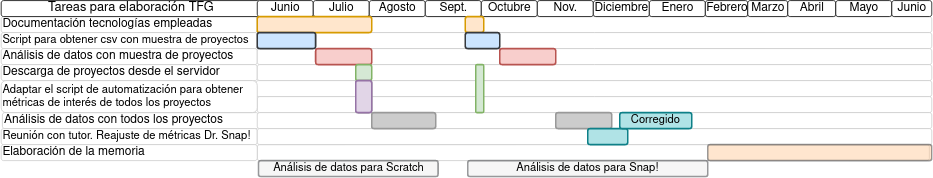
\includegraphics[width=\textwidth]{img/gantt}
    \caption{Diagrama de Gantt}
    \label{fig:gantt}
\end{figure}

%%%%%%%%%%%%%%%%%%%%%%%%%%%%%%%%%%%%%%%%%%%%%%%%%%%%%%%%%%%%%%%%%%%%%%%%%%%%%%%%
%%%%%%%%%%%%%%%%%%%%%%%%%%%%%%%%%%%%%%%%%%%%%%%%%%%%%%%%%%%%%%%%%%%%%%%%%%%%%%%%
% ESTADO DEL ARTE %
%%%%%%%%%%%%%%%%%%%%%%%%%%%%%%%%%%%%%%%%%%%%%%%%%%%%%%%%%%%%%%%%%%%%%%%%%%%%%%%%

\cleardoublepage
\chapter{Estado del arte}
\label{chap:estado}

\section{Scratch}
\label{sec:scratch}

Inspirado por Seymour Papert, del que fue doctorando y colaborador en los MIT Media Lab, Mitchel Resnick y su grupo de investigación \emph{Lifelong Kindergarten} comenzaron a desarrollar en 2003 el entorno web de programación Scratch\footnote{\url{https://scratch.mit.edu}}, que fue lanzado al público en mayo de 2007. En esta primera versión se buscaba dotar a los niños de una herramienta de aprendizaje con el que explorar sobre sus ideas en un proceso en ``espiral del pensamiento creativo''~\cite{resnick2008sowing}: se \emph{imagina} lo que se quiere hacer, se \emph{crea} y diseña un proyecto basado en esas ideas, para luego \emph{jugar} y experimentar con el programa creado, se \emph{comparte} con la comunidad de Scratch, recibiendo realimentación de otros que lo prueban y lo remezclan para sus propias creaciones en un entorno colaborativo, se \emph{reflexiona} y se vuelve a \emph{imaginar} en un proceso iterativo donde los proyectos se van refinando para resolver problemas cada vez más complejos~\cite{resnick2007all}.

Los cuatro principios sobre los que se apoya Scratch como herramienta de aprendizaje son: \textit{proyectos, pasión, compañeros y juego}~\cite{resnick2017seeds}. Está orientada a la creación de \emph{proyectos}, ya sean historias, animaciones, arte, música o videojuegos en función de los intereses y la temática que decida explorar el \emph{scratcher}. El niño programa para aprender de manera transversal competencias de cualquier disciplina. Al escoger y dar forma a un proyecto concreto según lo que les importa y les \emph{apasiona}, se comprometen, profundizan en conceptos y prácticas y se esfuerzan más en solventar los problemas y adversidades que surjan. Uno de los focos principales de Scratch es su comunidad online, donde se reciben consejos, mensajes y donde se aprende de \emph{compañeros}. Los proyectos compartidos son fuente de inspiración y pueden ser reinventados y remezclados. Los programadores de Scratch \emph{juegan} y experimentan con los objetos, indicando las acciones que deben realizar a través de bloques que arrastran, sueltan y encajan, para construir los distintos scripts que describen su comportamiento.
Van desarrollando la lógica de su proyecto, comprobando, depurando y mejorando su diseño.

Como lenguaje de programación Scratch se planteó conforme a 3 objetivos: \emph{``low floor, high ceiling, wide walls''}~\cite{resnick2009scratch}. Es sencillo iniciarse en la código-alfabetización a través de Scratch, puesto que los bloques presentan formas que indican cómo deben unirse y están organizados conforme a su funcionalidad en 9 categorías con colores distintos: movimiento, apariencia, sonido, eventos, control, sensores, operadores, variables y mis bloques. Esta última categoría fue añadida en la versión 2.0 y permite definir procedimientos o bloques propios, que junto a las listas y variables suponen un nivel superior de abstracción, para crear proyectos cada vez más complejos y modulares. Así el aprendiz moldea su aprendizaje, adquiere destrezas computacionales y da rienda suelta a su imaginación escogiendo, en un entorno diverso los casos de uso, extensiones y temas que mejor se adapten a sus inquietudes, vagaje y raíces culturales. En la figura~\ref{fig:road_trip} se observa el editor de Scratch con uno de los proyectos analizados en este trabajo de fin de grado. 

\begin{figure}
    \centering
    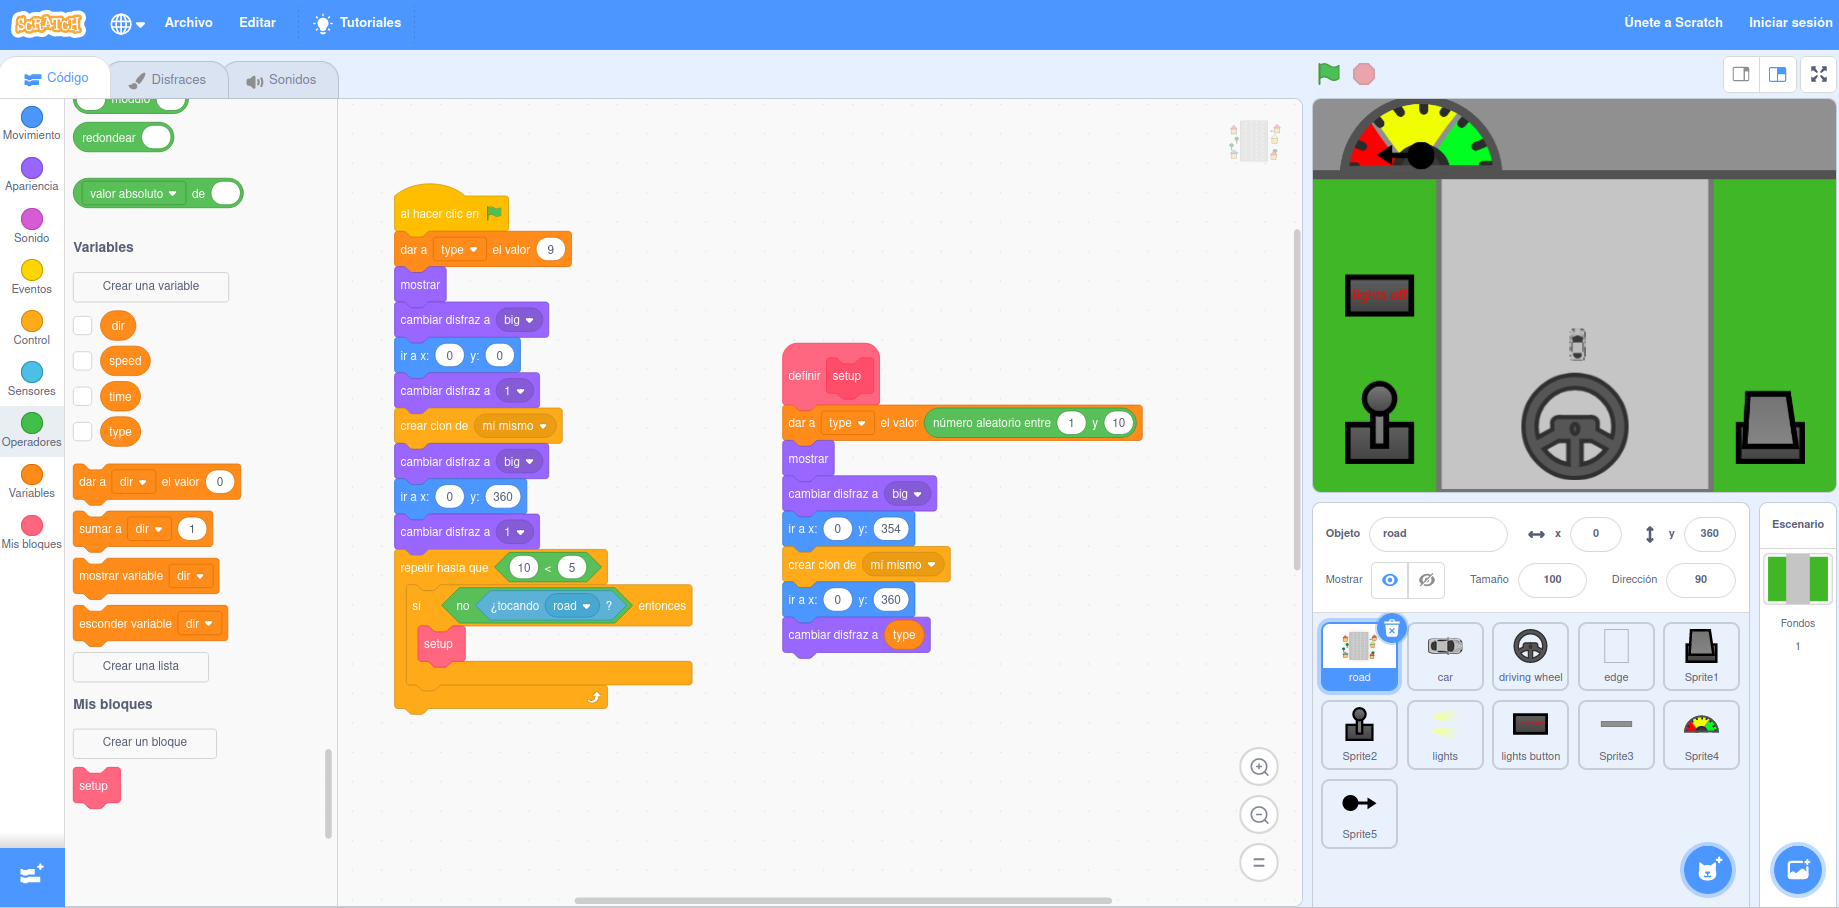
\includegraphics[width=.8\textwidth]{img/proy_Scratch}
    \caption{Proyecto de Scratch \emph{Road Trip} con funciones propias}\label{fig:road_trip}
\end{figure}
 
Scratch es el lenguaje de programación visual con fines educativos más extendido, con más de 91 millones de usuarios registrados de 200 países diferentes, que han compartido 105 millones de proyectos con la comunidad online\footnote{\url{https://scratch.mit.edu/statistics/}}. Es el resultado de incentivar el uso de Scratch en talleres, programas extracurriculares, centros comunitarios locales y Computer ClubHouses, hasta incluirlo en las etapas educativas obligatorias o K-12 como herramienta para adquirir las competencias digitales. La franja de edad más frecuente de los aprendices o \emph{tinkers} es de los 8 a los 16 años, como se aprecia en la figura~\ref{fig:edades}. %70 idiomas

\begin{figure}[H]
    \centering
    \begin{subfigure}[h]{.49\textwidth} 
        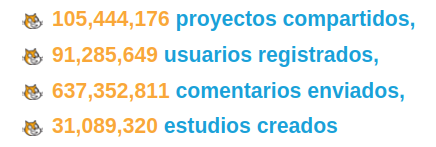
\includegraphics[width=\textwidth]{img/estad_Scratch}
        \caption{Magnitud y actividad de la comunidad}
        \label{fig:estad}
    \end{subfigure}       
    \begin{subfigure}[h]{.49\textwidth} 
        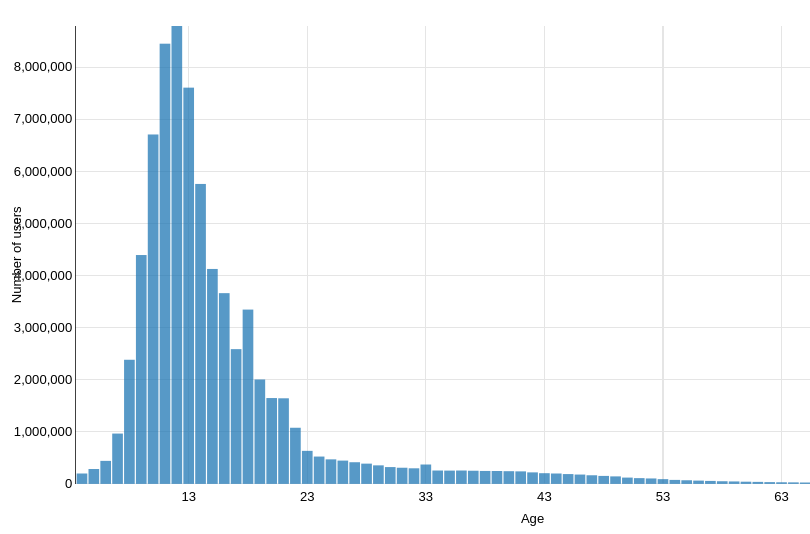
\includegraphics[width=\textwidth]{img/edades_Scratch}
        \caption{Distribución por edades nuevos scratchers}
        \label{fig:edades}
    \end{subfigure}
     \caption{Estadísticas de Scratch}
\end{figure} 

\section{Dr. Scratch}
\label{sec:dr_scratch}

Dr. Scratch\footnote{\url{http://www.drscratch.org}} es una aplicación web open-source que analiza proyectos programados en Scratch a través de su url o cargando el proyecto desde el ordenador. Los proyectos de la versión de Scratch 3.0 son almacenados en formato comprimido .sb3. Ya sea obteniendo el fichero de los servidores de Scratch o cargando el fichero JSON contenido en el directorio comprimido, analiza dicho fichero que contiene el código fuente del proyecto de Scratch e indica, a partir de los bloques utilizados en cada objeto, cuáles son las destrezas del pensamiento computacional demostradas en los proyectos. De manera automática el alumno, profesor u organización consiguen realimentación para mejorar en las áreas en las que menor puntuación obtenga, así como de las malas prácticas cometidas a la hora de programar~\cite{moreno2015dr, vargas2019bad}, pudiendo hacer un seguimiento de su progreso.

Ante la ausencia de herramientas que automatizaran la evaluación del pensamiento computacional, Gregorio Robles y Jesús Moreno se propusieron desarrollar la heramienta web libre de código abierto (FLOSS) 
Dr. Scratch en 2014. Inspirada por Scrape y tomando como base los plugins de Hairball, se extendió su funcionalidad para evaluar la calidad del código de los proyectos de Scratch y poder establecer el dominio del PC, tomando como referencia los métodos de evaluación de otros investigadores y las recomendaciones en los talleres organizados~\cite{moreno2015dr}. % Validez ecológica, convergente y discriminante. 

Los grupos de investigación GSyC-LibreSoft y KGB-L3 de la Universidad Rey Juan Carlos en colaboración con Programamos, así como doctorandos y alumnos han contribuido a que se despliegue la aplicación cliente - servidor en producción en una  máquina virtual alojada en Google Cloud Platform, a replicar e integrar la funcionalidad de Hairball y Kurt en la lógica de la aplicación para que analice los proyectos de Scratch 3.0~\cite{vargas2020analysis} y en adaptar la interfaz para que sea más intuitiva y adaptada al aprendizaje de los niños. 

\begin{table}
    \centering
    \resizebox{15cm}{!}{
    \begin{tabular}{|m{3.5cm}|m{4.5cm}|m{5cm}|m{5cm}|}
        \rowcolor[HTML]{CBCEFB}
        \textbf{Dimensión del PC} & \textbf{Básico} - 1 punto & \textbf{Intermedio} - 2 puntos & \textbf{Avanzado} - 3 puntos\\ \hline  
        \textbf{Abstracción} & Más de un script y más de un objeto. & Definición de bloques propios. & Uso de clones (o instancias de los objetos). \\ \hline
        \textbf{Paralelismo} & 2 scripts bajo el bloque de inicialización o evento bandera verde. &  2 scripts bajo los eventos: cuando se pulsa una tecla o sobre un objeto. & 2 scripts en: cuando recibe un mensaje, cuando cambia el escenario, o ante el mismo evento multimedia. \\ \hline
        \textbf{Pensamiento lógico} & if & if - else & Operadores lógicos \\ \hline
        \textbf{Sincronización} & Esperar & Enviar, cuando reciba mensaje, parar todos, parar programa, parar scripts del objeto. & Esperar hasta, cuando el escenario cambio a, enviar y esperar. \\ \hline
        \textbf{Control de flujo} & Secuencia de bloques. & Repetir n veces, por siempre. & Bucle repetir hasta. \\ \hline
        \textbf{Interactividad con el usuario} & Evento bandera verde. & Tecla u objeto pulsado, preguntar y esperar, eventos con el ratón. & Sensores de audio y vídeo. \\ \hline
        \textbf{Representación de los datos} & Modificadores de atributos de los objetos. & Funciones con variables. & Funciones con listas. \\ \hline
    \end{tabular}}
    \caption{Métricas de los niveles de competencia en cada dimensión del PC con Dr. Scratch~\cite{troiano19game}}
    \label{table:competence_level_Scratch}
\end{table}

Por lo tanto, en su última versión, se mantienen los 7 habilidades computacionales analizadas en el código de cada proyecto y las métricas que asignan a cada uno de ellos una valoración entera entre 0 y 3. La abstracción y descomposición de problemas, el paralelismo, el pensamiento lógico, la sincronización, nociones algorítmicas de control de flujo, la interactividad con el usuario y la representación de los datos quedan definidas como se indica en la tabla~\ref{table:competence_level_Scratch}. Se suman sus valores y se indica al aprendiz cuál es su puntuación total en el desarrollo del pensamiento computacional.

A partir de esa complejidad global del proyecto se establecen tres niveles de destreza: básico, intermedio y avanzado. Al ser una herramienta formativa-iterativa~\cite{roman2019combining} y de ludificación basada en retos, busca involucrar al programador y ayudarle a desarrollar las dimensiones en que obtenga peores resultados. Por ello, proporciona enlaces con ejemplos de como mejorarlas, estadísticas y gráficas con su progreso y consejos de como evitar los malos hábitos en programación detectados, únicamente cuando va avanzando de nivel, así como la obtención de medallas y certificados. En la figura~\ref{fig:dashboards} se distinguen las diferencias en la realimentación proporcionada según el nivel alcanzado.

\begin{figure}[H]
    \centering
    \begin{subfigure}[h]{.325\textwidth} 
        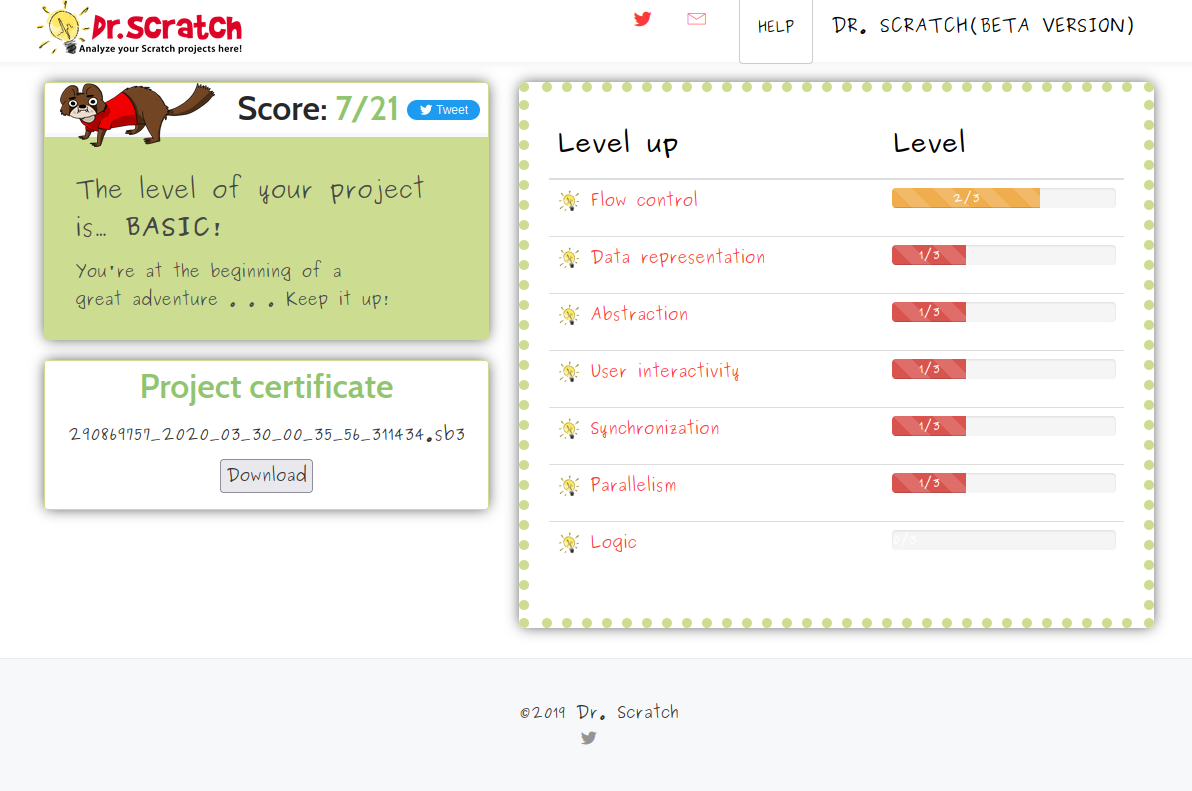
\includegraphics[width=\textwidth]{img/basico_Scratch}
        \caption{Nivel básico: [0, 7] puntos}
    \end{subfigure}       
    \begin{subfigure}[h]{.325\textwidth} 
        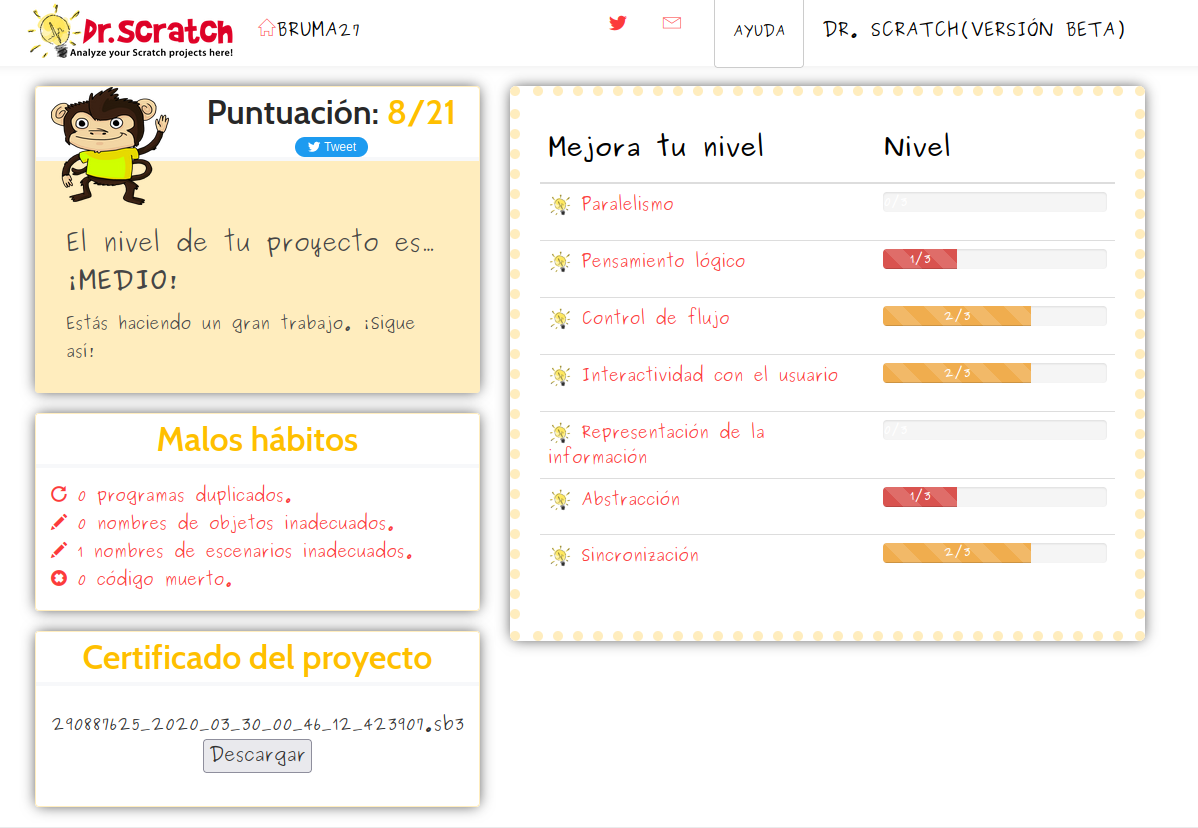
\includegraphics[width=\textwidth]{img/medio_Scratch}
        \caption{Nivel intermedio: [8, 14]}
    \end{subfigure}
    \begin{subfigure}[h]{.325\textwidth} 
        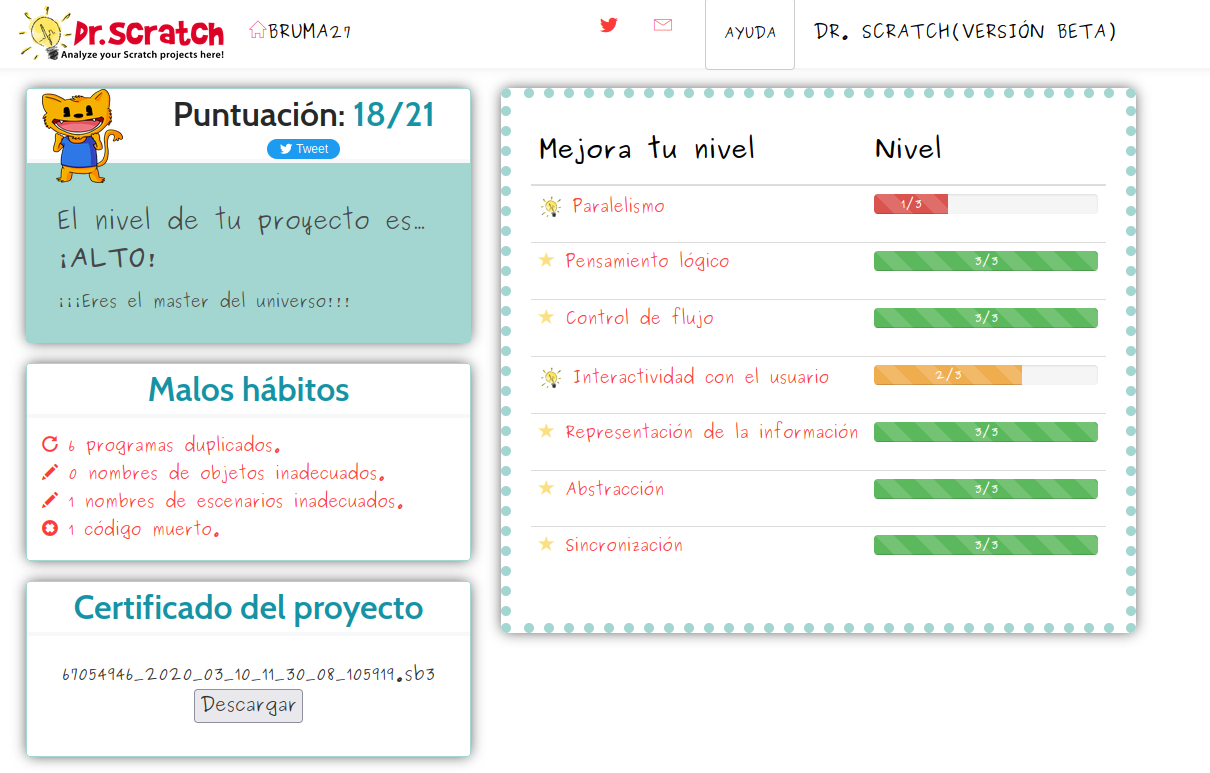
\includegraphics[width=\textwidth]{img/alto_Scratch}
        \caption{Nivel avanzado: [15, 21]}
    \end{subfigure}
    \caption{Dashboards de Dr. Scratch según valoraciones totales asignadas a cada nivel}
    \label{fig:dashboards}
\end{figure}

Dr. Scratch se utiliza a escala mundial por organizaciones, investigadores, profesores que analizan los proyectos creados por sus alumnos, y por los mismos jóvenes programadores, ofreciendo distintos perfiles para cada usuario y la posibilidad de elegir entre 9 idiomas disponibles. Este servicio web analiza estáticamente más de 10.000 proyectos al mes y fue galardonada con el Google Rise Award en 2015. % Versión alpha, versión beta , adaptación a proyectos de Scratch .sb3

\section{Snap!}
\label{sec:snap}

Snap!\footnote{\url{https://snap.berkeley.edu/}} es un lenguaje de programación visual con bloques cuya primera versión fue desarrollada en 2008 por Jens Mönig y Brian Harvey. Denominada en sus orígenes \emph{BYOB, ``Build Your Own Blocks''}, extendía la funcionalidad de la versión 1.4 de Scratch incluyendo la posibilidad de definir procedimientos o funciones propias. Se puede elegir la categoría a la que pertenecen de las 8 disponibles y si el bloque definido, encapsulado como una primitiva, será utilizado por el objeto donde se declara o por todos los objetos del proyecto.
Estos bloques propios tienen forma de comando, si es una instrucción o procedimiento, de reportero cuando es una función que devuelve un valor o de condición si devuelve un booleano. Por ello permite la recursividad, como la que se aplica en el proyecto de Snap! de la figura~\ref{fig:fractal}.

\begin{figure}[H]
    \centering
    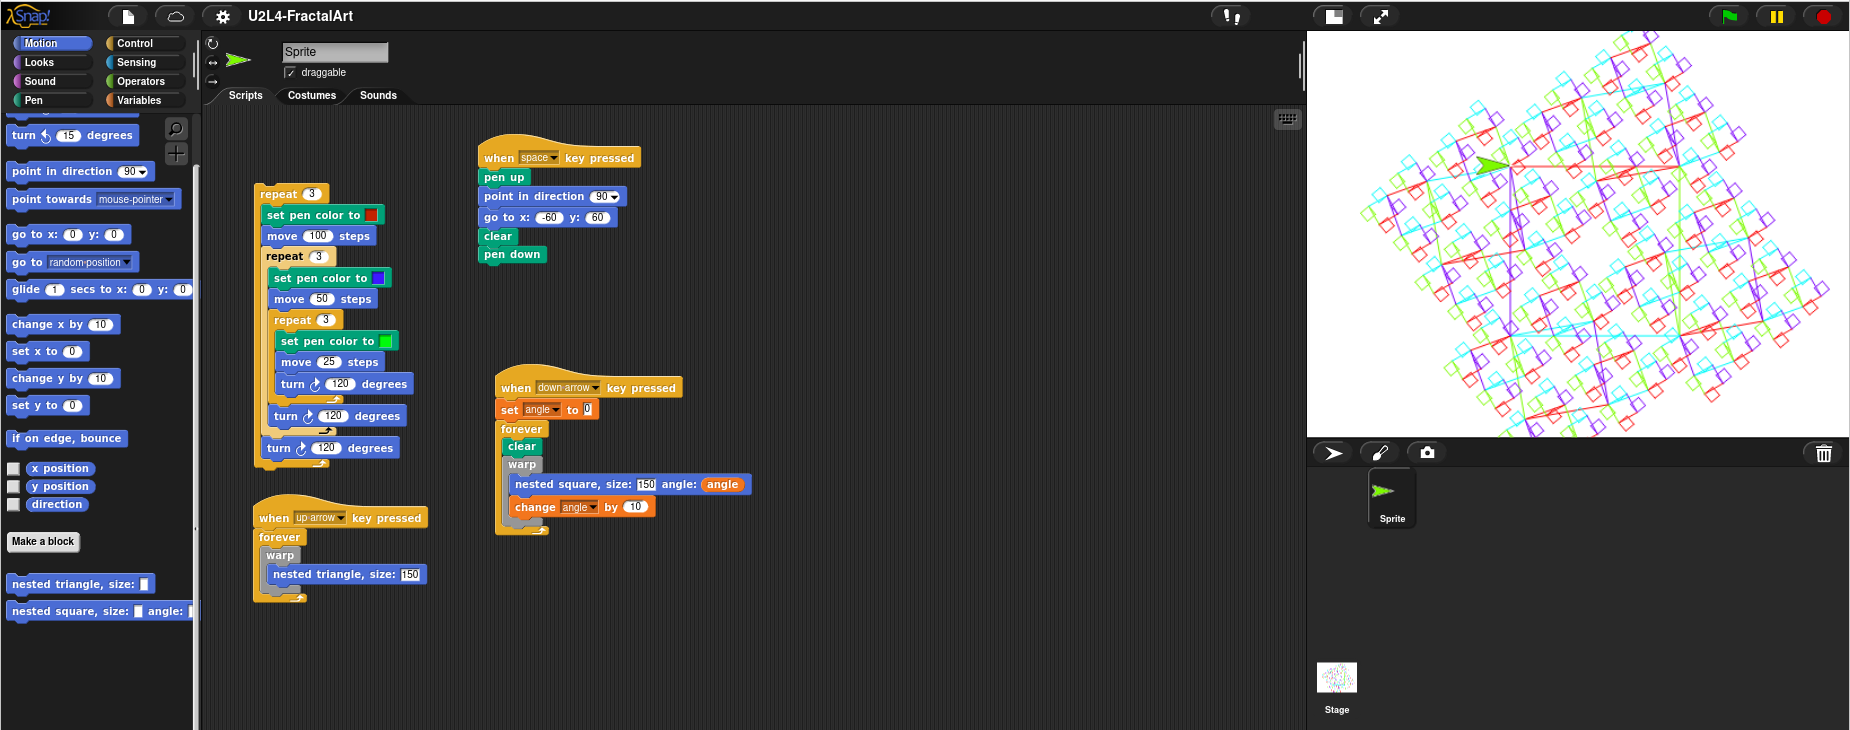
\includegraphics[width=1\textwidth]{img/proy_Snap.png}
    \caption{Proyecto de Snap! \emph{U2L4-FractalArt}, tomado del conjunto de proyectos analizados}
    \label{fig:fractal}
\end{figure}

Según B. Harvey ``Snap! es Scheme disfrazado de Scratch''~\cite[p. 3]{harvey2017snap}, por lo que todos los tipos de datos son de primera clase, las listas, los procedimientos, las continuaciones, los objetos, los disfraces y los sonidos. De esta manera se pueden tener listas enlazadas, diccionarios, listas de listas o estructuras de datos heterogéneas cuyos elementos pueden ser de cualquier tipo. Los anillos grises permiten crear expresiones $\lambda$ a partir de bloques o scripts, para utilizarlas como parámetro o resultado de funciones de orden superior.
Por lo tanto, los programadores pueden experimentar con herramientas propias de la programación funcional, profundizando en conceptos abstractos y de diseño~\cite{harvey2015lambda}.
Como muestra de la relevancia que adquiere en Snap! este paradigma, tanto su logo como su mascota Alonzo, el antiguo Gobo de Scratch, incluyen una $\lambda$ en honor al cálculo lambda de Alonzo Church.

No obstante, Snap! permite un enfoque imperativo y una programación orientada a objetos basada en prototipos por delegación, orientado a las simulaciones. A diferencia de Scratch, un objeto puede enviar un mensaje a otro objeto en particular y los clones pueden añadir sus propios atributos, tras heredar todos los atributos del objeto padre~\cite{snap2022git}. % versión 5 -> blocks for analyzing data and transforming media: https://dl.acm.org/doi/abs/10.1145/3328778.3372549. 

Mientras que en Scratch 2.0 optaron por mantener el software privativo Flash Player para el contenido multimedia de los proyectos de sus usuarios hasta el desarrollo de la versión 3 en 2019, en la versión 4 de Snap! se decidió reimplementar BYOB en JavaScript usando el lenguaje de marcado HTML5. En consecuencia, se puede acceder a Snap! desde cualquier navegador, con independencia del SO. Los usuarios registrados pueden almacenar sus proyectos de Snap! en un servidor en la nube de forma privada o pueden decidir compartirlos o publicarlos en el sitio web de Snap! Está menos orientado que Scratch a la interacción entre los miembros de su comunidad, por lo que no incide en la remezcla y ofrece menos tutoriales. De hecho la comunidad de Snap! posee una incidencia drásticamente menor, contando en marzo de 2021 con 511.000 cuentas de usuario con 4.525.000 proyectos creados, de los cuales sólo el 37\% habían sido compartidos\footnote{\url{https://forum.snap.berkeley.edu/t/how-many-snap-users-are-there/5598/7}}. Está dirigido a jóvenes entre 14 y 20 años~\cite{harvey2013snap}. %%
 
\section{Dr. Snap!}
\label{sec:dr_snap}

Dr. Snap! es una aplicación web desarrollada por Paula Rodríguez en su trabajo de fin de grado~\cite{martinez2021dr}, con el propósito de analizar la asimilación de conceptos y prácticas del pensamiento computacional a partir de los proyectos de Snap! creados por los estudiantes. A partir de la url del proyecto obtiene su código fuente en formato XML de los servidores en la nube de Snap!\footnote{\url{https://cloud.snap.berkeley.edu}}. Se parsea y se carga en un fichero JSON los datos de variables y bloques empleados en cada script o función de los objetos, que permiten determinar cada una de las 8 dimensiones del PC.

Siguiendo la estela marcada por Dr. Scratch, se mapean los datos obtenidos en el documento JSON a una puntuación entera entre 0 y 3 para cada competencia. En la tabla~\ref{table:competence_level_Snap}, se perciben ligeras diferencias en abstracción, paralelismo, sincronización e interactividad con el usuario. Condicionales es equivalente al pensamiento lógico de Dr. Scratch. Se incluye diversidad como métrica que mide la complejidad del proyecto de Snap! en función del uso de bloques de distintas categorías, las cuales tienen un color asociado y son: movimiento, apariencia, sonido, lápiz, control, sensores, operadores y variables.

\begin{table}
    \centering
    \resizebox{15cm}{!}{
    \begin{tabular}{|m{3.5cm}|m{4.5cm}|m{5cm}|m{5cm}|}
       \rowcolor[HTML]{CBCEFB}
       \textbf{Dimensión del PC} & \textbf{Básico} - 1 punto & \textbf{Intermedio} - 2 puntos & \textbf{Avanzado} - 3 puntos\\ \hline
       \textbf{Abstracción} & Más de un script. & Más de un script y más de un objeto. & Definición de bloques propios. \\ \hline
       \textbf{Paralelismo} & Un objeto ejecuta 2 o más scripts ante los eventos: bandera verde o pulsar una tecla. & 2 objetos ejecutan 1 o más scripts a la vez ante los eventos: bandera verde o pulsar una tecla. & Eventos: cuando reciben un mensaje, cuando se cumple una condición o cuando usan clones. \\ \hline
       \textbf{Condicionales} & if & if - else & Operadores lógicos \\ \hline
       \textbf{Sincronización} & Esperar. & Enviar, cuando reciba mensaje, parar todos, parar script. & Esperar hasta, enviar y esperar, cuando se cumple condición o empiece como clon. \\ \hline
       \textbf{Control de flujo} & Secuencia de bloques. & Repetir n veces, por siempre. & Bucles for o repetir hasta. \\ \hline
       \textbf{Interactividad con el usuario} & Eventos: bandera verde o pulsar una tecla. & Sensores:   
       tecla u objeto pulsado. Eventos con el ratón sobre el objeto. & Preguntar y esperar, detección de colisiones, sensores de audio y vídeo. \\ \hline
       \textbf{Representación de los datos} & Modificadores de atributos de los objetos. & Funciones con variables. & Funciones con listas. \\ \hline
       \textbf{Diversidad} & $\leq2$ categorías de bloques & $2<$ categorías $\leq6$ & $\geq7$ categorías de bloques\\ \hline
    \end{tabular}}
    \caption{Métricas de los niveles de competencia en cada dimensión del PC con Dr. Snap!~\cite{martinez2021dr}}
    \label{table:competence_level_Snap}
\end{table}

El análisis estático que pondera cada proyecto, le otorga una valoración global entre 0 y 3, que es la media conseguida a partir de las 8 dimensiones. Con ella se asigna una etapa de desarrollo del pensamiento computacional según los siguientes rangos: en [0, 0.5) el nivel es nulo, en [0.5, 1.5) el nivel es básico, en [1.5, 2.5) el nivel es intermedio y en [2.5, 3] se controla por completo esta aptitud cognitiva. Las páginas de respuesta al usuario según esta distinción se muestran en la figura~\ref{fig:dashboards_Snap}.

\begin{figure}[H]
    \centering
    \begin{subfigure}[h]{.325\textwidth} 
        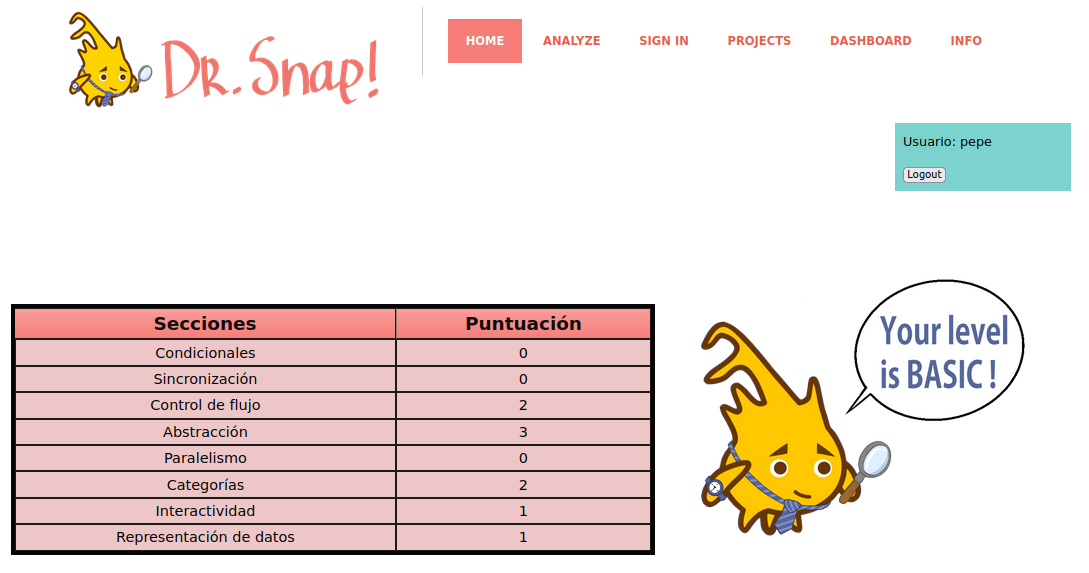
\includegraphics[width=5.5cm,height=5.5cm,keepaspectratio]{img/basico_Snap}
        \caption{Nivel básico}
    \end{subfigure}       
    \begin{subfigure}[h]{.325\textwidth} 
        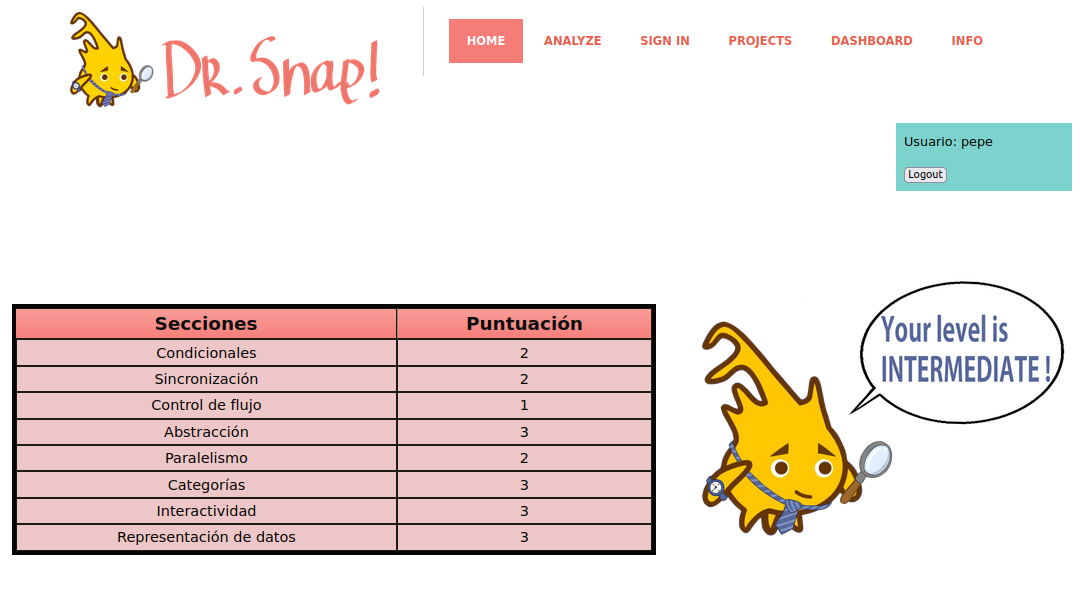
\includegraphics[width=5.5cm,height=5.5cm,keepaspectratio]{img/medio_Snap}
        \caption{Nivel intermedio}
    \end{subfigure}
    \begin{subfigure}[h]{.325\textwidth} 
        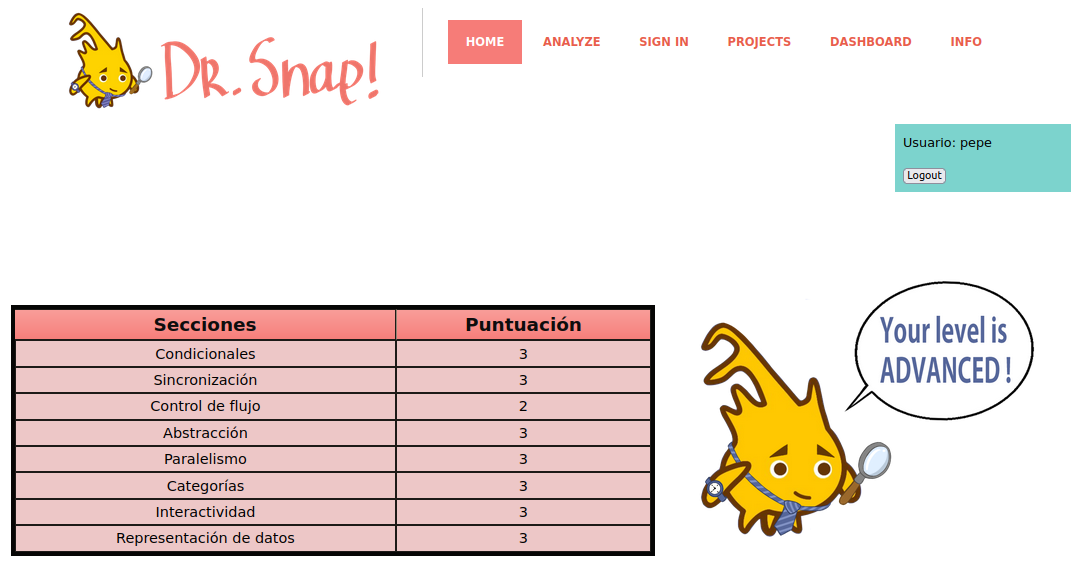
\includegraphics[width=5.5cm,height=5.5cm,keepaspectratio]{img/alto_Snap}
        \caption{Nivel avanzado}
    \end{subfigure}
    \caption{Páginas de Dr. Snap! según puntuaciones totales asignadas a cada nivel}
    \label{fig:dashboards_Snap}
\end{figure}

Si el usuario está autenticado podrá hacer seguimiento de la etapa de desarrollo en la que se encuentran los proyectos analizados. En el caso de que sea profesor, puede subir un archivo comprimido con todos los proyectos de su clase y determinar las capacidades en que sus alumnos obtengan peores resultados, para incidir en ellas si así se requiere. También se pueden comparar dos conjuntos de proyectos en un diagrama de barras, para observar la evolución de sus alumnos según avanzan las clases o fijar las diferencias entre dos grupos de test distintos. Se facilita de este modo su labor docente.

\section{Python}
\label{sec:python}
Python\footnote{\url{https://www.python.org}} es un lenguaje de programación de alto nivel, interpretado, multiparadigma, aunque con un marcado enfoque hacia la programación orientada a objetos. Fue desarrollado por Guido van Rossum entre diciembre de 1989 y febrero de 1991, fecha en que la primera versión estuvo disponible~\cite{van2007python}. La última versión estable es la 3.10.4.

Entre sus principios de diseño priman la legibilidad en su sintaxis, la sencillez, ser compacto, explícito, conciso, con estructuras planas~\cite{peters2010zen} y busca mejora la productividad. Es relativamente sencillo empezar a programar en Python y tiene una curva de aprendizaje moderada. Por ello, es una poderosa herramienta de aprendizaje para el pensamiento computacional~\cite{wang2021research}.

Es multiplataforma, puesto que permite su ejecución en cualquier sistema operativo. Es de propósito general, contando con una extensa colección de bibliotecas y módulos aplicables al desarrollo web, a la ciberseguridad o a la ciencia y análisis de datos. Todo ello conlleva a que sea uno de los lenguajes más utilizados. 

\section{Jupyter Notebooks}
\label{sec:jupyter}

En el contexto del proyecto IPython surgió en 2014 el proyecto Jupyter \footnote{\url{https://jupyter.org}}, cuyos fundadores son Fernando Pérez y Brian Granger. Es un ecosistema que aboga por el desarrollo de herramientas open-source bajo la licencia BSD modificada, dedicadas a la computación interactiva. 

Jupyter Notebook es una aplicación web cliente-servidor que proporciona una interfaz gráfica que permite la programación interactiva en el navegador, pudiendo incluir los resultados de la ejecución de cada celda, documentación en varios formatos, fórmulas con LaTeX, imágenes, gráficos y contenido multimedia en un mismo documento Jupyter. Se pueden compartir los resultados de esta narrativa computacional y recopilar todos los ficheros de un proyecto en su dashboard, así como cuadernos ejecutados en lenguajes como Julia, Python y R, siendo muy útil para investigadores, educadores y científicos de datos~\cite{perez2015project}.

\section{NumPy} 
\label{sec:numpy}

NumPy, \emph{Numerical Python}\footnote{\url{https://numpy.org}}, es la biblioteca open-source de bajo nivel que almacena y opera con datos homogéneos tomados como arrays multidimensionales y matrices de manera más eficiente. Fue desarrollada por Travis E. Oliphant en 2006~\cite{oliphant2006guide}.

Sirve como base para el procesado y tratamiento de texto, audio o imágenes e integra un conjunto de atributos y métodos que la convierten en el paquete fundamental para la investigación y computación científica con Python. En particular, es el núcleo que sirve de soporte a otras bibliotecas de alto nivel en la ciencia y análisis de datos~\cite{harris2020array}, como las expuestas a continuación.

\section{Pandas} 
\label{sec:pandas}

Wes McKinney inició el desarrollo de esta biblioteca de Python en 2008 en la entidad financiera AQR. Desde 2009 es un proyecto open-source mantenido por la comunidad de Pandas\footnote{\url{https://pandas.pydata.org/about}}. Su nombre proviene de las estructuras de datos tridimensionales empleadas en estadística y econometría conocidas como \emph{Panel Data}~\cite{mckinney2011pandas}.

Es un módulo de alto nivel construido sobre NumPy cuyos objetos son las series y los dataframes, un conjunto de datos heterogéneos indexados organizados en tablas con tantas filas como observaciones y tantas columnas como variables a analizar. Estos datos provienen de bases de datos relacionales o de hojas de cálculo. Reúne un conjunto de métodos y funciones avanzadas que permiten cargar, limpiar, ordenar, filtrar, agrupar y manipular los datos para facilitar el análisis~\cite{McKinneyWes2018Pfda, VanderplasJake2017Pdsh}. % Aúna lo mejor de los dos mundos.

\section{Matplotlib} 
\label{sec:matplotlib}

Matplotlib\footnote{\url{https://matplotlib.org}} es una biblioteca open-source multiplataforma creada por John D. Hunter en 2003 como alternativa a Matlab en Python~\cite{Hunter2007}. Dentro del ecosistema de la programación científica se construye sobre NumPy y es de bajo nivel.
Sirve para la representación y la visualización de gráficos matemáticos y estadísticos de alta calidad en 2D y 3D, ya sean estáticos, dinámicos o animaciones. Permite su integración en entornos gráficos interactivos como el de Jupyter o en aplicaciones web~\cite{VanderplasJake2017Pdsh}.

Si bien posee una API orientada a objetos para personalizar y realizar operaciones avanzadas sobre el contenedor de las figuras y sus ejes, su módulo \texttt{pyplot}, más parecido a Matlab, simplifica la representación. 

\section{Seaborn} 
\label{sec:seaborn}

Seaborn\footnote{\url{http://seaborn.pydata.org}} es una biblioteca de Python de alto nivel basada en matplotlib, orientada a la representación de gráficos estadísticos. Su API facilita la exploración y visualización de datos, proporcionando funciones que trabajan directamente con las series y los dataframes de Pandas pasados como parámetros, realizando internamente las estimaciones estadísticas requeridas y presentando los gráficos solicitados, debidamente etiquetados, con diseños más atractivos que matplotlib~\cite{waskom2021seaborn}.

\section{Scikit-Learn} 
\label{sec:sklearn}

David Cournapeau inició el proyecto Scikit-Learn en el Google Summer of Code en 2007. Matthieu Brucher se unió en 2008. En 2010 se publicó su primera versión\footnote{\url{https://scikit-learn.org/stable/about.html}}. Actualmente es una biblioteca open-source bajo licencia BSD desarrollada por colaboradores internacionales, coordinada y mantenida principalmente por un equipo de investigadores del Inria \emph{(French Institute for Research in Computer Science and Automation)}.

Con dependencias de NumPy y SciPy, es una API de propósito general que facilita la aplicación de algoritmos de Machine Learning supervisado y no supervisado e incluye módulos de preprocesamiento de datos, comparación, validación y selección de modelos y reducción de dimensionalidad~\cite{pedregosa2011scikit}. Su API está diseñada para ser simple, eficiente, accesible para investigadores de diversa áreas y reutilizable. Está compuesta por tres interfaces: de transformación de los datos representados como arrays de numpy, de estimación para crear y entrenar los modelos y de predicción. Sus principios de diseño son: consistencia en los objetos, inspección de atributos públicos, no proliferación de clases, composición y valores predeterminados sensibles~\cite{sklearn_api}.



%%%%%%%%%%%%%%%%%%%%%%%%%%%%%%%%%%%%%%%%%%%%%%%%%%%%%%%%%%%%%%%%%%%%%%%%%%%%%%%%
%%%%%%%%%%%%%%%%%%%%%%%%%%%%%%%%%%%%%%%%%%%%%%%%%%%%%%%%%%%%%%%%%%%%%%%%%%%%%%%%
% DISEÑO E IMPLEMENTACIÓN %
%%%%%%%%%%%%%%%%%%%%%%%%%%%%%%%%%%%%%%%%%%%%%%%%%%%%%%%%%%%%%%%%%%%%%%%%%%%%%%%%

\cleardoublepage
\chapter{Diseño e implementación}
\label{chap:diseño_implementación}

%``Es mejor tener una respuesta aproximada a la pregunta correcta, que una respuesta exacta a la pregunta equivocada''. J. W. Tukey.
En la fase de documentación se estudiaron las distintas tecnologías comentadas en el capítulo~\ref{chap:estado}, para conocer las métricas que ponderan el desarrollo del pensamiento computacional tanto en Dr. Scratch como en Dr. Snap! El objetivo era extraer patrones, tendencias y relaciones entre las habilidades a partir de un volumen de proyectos suficientemente amplio y representativo de ambas poblaciones para así poder compararlas. Se recurre a un análisis de datos descriptivo cuantitativo para explorar y conocer la información que se desprende al aplicar técnicas estadísticas y de visualización de datos. Se muestra en la figura~\ref{fig:diseño} el proceso y el diseño del script implementado. Lo obtenido en cada paso acota las herramientas a emplear en el siguiente.

\begin{figure}[H]
    \centering
    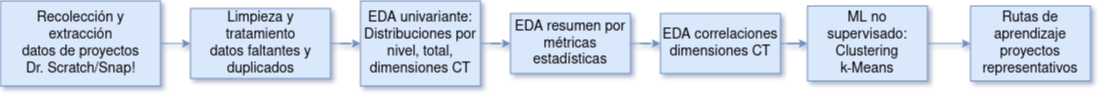
\includegraphics[width=1.0\textwidth]{img/diseno_script_2.png}
    \caption{Diagrama del proceso de análisis de datos}\label{fig:diseño}
\end{figure}

Para ambos análisis se debían recolectar los proyectos almacenados en una base de datos e implementar un script que automatizara la recogida de las métricas de cada proyecto, las guardara en un fichero CSV para, posteriormente, cargarlo con Pandas y realizar el análisis de datos en los Jupyter Notebooks. Para completar la preparación de los datos se requiere eliminar datos espurios que distorsionen su comprensión, descartando de la muestra los proyectos duplicados o con atributos incompletos. Se formatean mediante la conversión de tipos de las variables o columnas que los caracterizan, que facilite su estudio estadístico, su representación gráfica y el entendimiento de lo que representan.

En la tercera etapa se comienza a conocer cómo se distribuyen los proyectos en función del nivel alcanzado, la valoración total conseguida y las puntuaciones obtenidas en cada unas de las siete habilidades del pensamiento computacional. Se filtran, combinan y agrupan los valores de las columnas para analizar la competencia demostrada general y particular para cada destreza considerada de las ciencias de la computación. 

Posteriormente, se calculan los estadísticos que resumen las propiedades de las variables en cuanto a tendencia central, dispersión y posición, pudiendo perfilar que habilidades resultan más fáciles y si sus métricas están muy concentradas. 

Se completa el análisis exploratorio de datos (EDA) tratando de encontrar las relaciones y dependencias entre las habilidades gracias a las correlaciones, considerando todos los proyectos y desglosándolos según la puntuación total conseguida, para ver su evolución según aumenta la complejidad de los proyectos.

Para descubrir similitudes entre los proyectos ocultas a simple vista, se aplica un modelo de aprendizaje no supervisado, el clustering K-Means. Segmenta la totalidad de los proyectos en k grupos, aplicando un criterio de mínima distancia al centro del grupo, según su posición definida por las siete dimensiones. Se estima el valor de k, ya sea con herramientas de validación externa o con índices que relacionan las distancias intra-clúster o inter-clúster, escogiendo el valor de k que los minimice o los maximice, según sea el caso, o donde convergan diferentes criterios. Una vez tenemos el valor de k, se ejecuta iterativamente el algoritmo K-Means hasta encontrar la posición óptima de los proyectos representativos del grupo. Éstos pueden interpretarse como prototipos en el proceso de aprendizaje.

\section{Recolección y extracción de datos}  
\label{sec:collect_data}

Cuando se analiza con Dr. Scratch un proyecto, ya sea a través de su url o cargando el proyecto de Scratch desde el ordenador, se almacena una copia del proyecto en la base de datos MySQL en los formatos comprimidos propios de Scratch, según la versión de Scratch utilizada para implementarlo. La mayoría de los proyectos pertenecen a la versión 3.0 de Scratch que se corresponde con la extensión .sb3. No obstante, algunas de las copias salvadas cuentan con extensiones .sb2 y .sb, vinculadas a versiones antiguas. 

Se accedió al servidor en remoto vía ssh mediante clave pública-privada para descargar los 271.558 proyectos de Scratch que se encontraban en el directorio \texttt{drscratchv3/uploads/}. Ocupaban cerca de 80GB y estaban fechados entre el 1 junio de 2019 y el 31 de julio de 2021. Se fueron copiando por lotes en local, gracias a scp y rsync, en función del mes y año. 

El módulo \texttt{analyzer} de Dr. Scratch asigna puntuaciones a cada una de las 7 habilidades del pensamiento computacional en función de los bloques empleados. Para ello, analiza el documento JSON que almacena el código fuente de cada proyecto, ubicado en el directorio comprimido. Se adaptó el módulo para que pudiera ser ejecutado desde línea de comandos como programa principal, pasándole como argumento el proyecto de Scratch a analizar (en formato comprimido .sb*) o la ruta al mismo. Se modificó para que imprimiera por pantalla las métricas de cada habilidad, el total obtenido al sumarlas y la valoración media para cada proyecto, en una fila separada por comas. Se redirigió la salida estándar al fichero \emph{results.csv}.  
Con un bucle for en bash scripting se automatizó el análisis para todos los lotes de proyectos, indicando el path al directorio donde se localizan. El flujograma del script se representa en~\ref{fig:script_extract}.

Aquellos proyectos que generaban excepciones por fallos en la descompresión del proyecto, en la conversión del objeto JSON a un diccionario o en el acceso y obtención de elementos o claves al recorrer la estructura de diccionarios anidados, fueron registrados redirigiendo el flujo de errores estándar, \emph{stderr}, al fichero \emph{error.csv}. Este fichero indicaba la ruta al proyecto, el tipo de excepción capturada y la línea donde se produce. Contenía 1.714 proyectos excluidos del análisis de datos posterior.

\begin{figure}[ht]
    \centering
    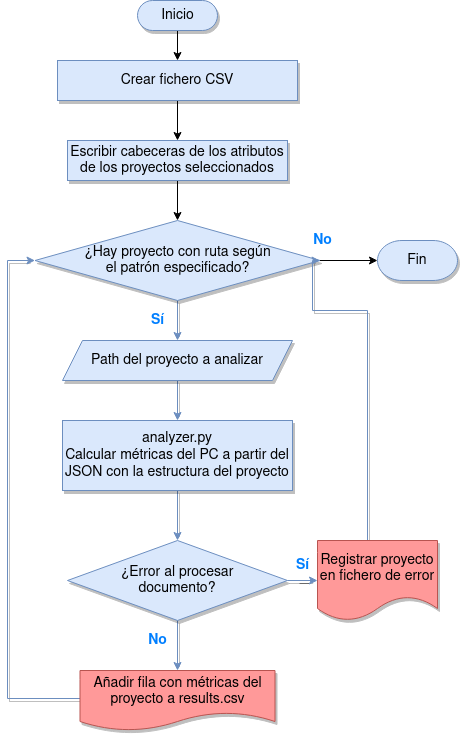
\includegraphics[height=.6\textheight]{img/script_extraccion_datos.png}
    \caption{Diagrama de flujo del script get\_csv}
    \label{fig:script_extract}
\end{figure}

Para los proyectos de Snap!, mi tutor, Gregorio, me pasó un enlace a un archivo comprimido. Se transfirió su contenido a un disco duro externo. El directorio generado ocupaba 31,9 GB e incluía 113.906 proyectos almacenados cada uno en un directorio distinto.

Para extraer la información seleccionada de esta fuente de datos se codificó un script de python, \texttt{get\_csv.py} cuyo diagrama se muestra en~\ref{fig:script_extract}. Si se ejecuta como programa principal, se crea el fichero \emph{result\_snap\_metrics.csv}. Gracias a la biblioteca \texttt{glob}, se recorre una lista con las rutas a los proyectos de Snap! conforme a un patrón específico y se van rellenando las filas del CSV para cada proyecto según los atributos escogidos. Para ello llama a la función \texttt{calcular\_puntuacion()} del módulo \texttt{analyzer}. Este módulo recogía las funciones encargadas de calcular el desarrollo del PC de la lógica de la aplicación web de Dr. Snap! Se adaptó para que el parámetro de entrada de la función \texttt{calcular\_puntuacion(file\_xml)} no sea la url, sino el path del proyecto Snap! a analizar, almacenado como documento XML en un árbol de directorios contenidos en un disco duro externo. Se extrajo a otro módulo la parte encargada de parsear el documento XML, que describe la estructura del código fuente del proyecto solicitado al servidor de Snap! Berkeley. 

En el módulo \texttt{parser} se importa el módulo estándar \texttt{xml.sax}. Se genera un parser SAX que procesa el documento como un stream, de manera que el parser genérico creado lee eventos de interés según se van produciendo, y llama a métodos concretos del manejador que especifican qué hacer cuando encuentra determinadas etiquetas anidadas dentro del nodo raíz o elemento project y cómo tratar algunos de sus atributos. En concreto, guarda el nombre del proyecto, los nombres de los bloques utilizados en cada script contenido dentro de un personaje o sprite, los nombres de los bloques personalizados o funciones propias definidas por el programador, así como los bloques utilizados para su implementación y los nombres de las variables declaradas. Además realiza un recuento de las etiquetas sprite, script, bloque, bloque personalizado y variable que aparecen en el documento XML del proyecto. Esta información se almacena en variables del objeto hasta que el parser encuentra el fin de la etiqueta project. Llama al método de la clase del manejador endElement y se almacenan los datos en un documento JSON.

Se define una clase \texttt{ParserXML} cuyo constructor consta de dos atributos: un objeto que es el parser genérico creado a partir de \texttt{make\_parser()} y un manejador que instancia un objeto de la clase \texttt{myContentHandler}, que hereda a su vez de la clase \texttt{ContentHandler} predefinida en el módulo \texttt{handler} de la biblioteca xml.sax. Se vincula el parser con el manejador modificado, para que cuando encuentre eventos de contenido, se desencadene la ejecución de los métodos del manejador con la extensión de funcionalidad indicada anteriormente, tomada de Dr. Snap! La clase recibe como parámetro de entrada la ruta del documento XML con la estructura del proyecto codificado en Snap!, almacenado en el disco duro externo. El parser analiza el fichero XML según el comportamiento indicado en el manejador, salvo que localice en el flujo de datos errores en la sintaxis del XML, caracteres terminales no permitidos o \emph{invalid\_token}. En ese caso el proyecto se registra en un fichero donde se indica el tipo de error que se produce y en qué punto salta la excepción. Todos los documentos XML mal formados fueron corregidos. 

Cuando se llama a \texttt{calcular\_puntuacion} desde el módulo principal \texttt{get\_csv}, se instancia un objeto de la clase \texttt{ParserXML} que devuelve un fichero en formato JSON, con el contenido que nos interesa en una estructura de datos más compacta, legible y ligera. Se convierte en un diccionario de listas, que es el parámetro de entrada de las funciones que analizan las habilidades del pensamiento computacional en función de los bloques utilizados en los proyectos, el número de scripts y el número de sprites. Se corrigieron duplicidades y se mejoró el código del módulo \texttt{analyzer}.

\section{Limpieza y tratamiento de datos} 
\label{sec:clean_data}

A pesar de que se ha tenido especial cuidado en la fase de obtención y selección de datos a partir de ambas fuentes, el script de automatización puede recoger proyectos con campos vacíos o proyectos duplicados. Además es conveniente homogeneizar los datos y ajustar los tipos de las variables que los caracterizan. De esta manera se depuran los datos en crudo obtenidos de \emph{results.csv} y \emph{result\_snap\_metrics.csv} y cargados en la estructura de datos bidimensional o dataframe en sendos \emph{Jupyter Notebooks}\footnote{https://github.com/rcruiz/pruebaCT/blob/main/Dr\_Scratch\_Analysis.ipynb} \footnote{https://github.com/rcruiz/DrSnap-Analysis/blob/main/Dr\_Snap\_complete\_analysis.ipynb}. El proceso seguido en esta segunda etapa se muestra en la figura~\ref{fig:script_clean}. 

\begin{figure}[ht]
    \centering
    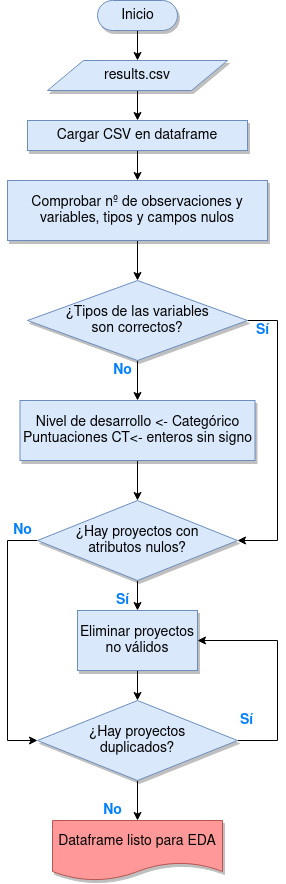
\includegraphics[height=.6\textheight]{img/script_clean2.png}
    \caption{Diagrama de flujo: limpieza de datos}\label{fig:script_clean}
\end{figure}

A partir de este script se obtienen 269.842 proyectos de Scratch y 113.894 proyectos de Snap! únicos y válidos con un nivel asignado de tipo categórico y cuyas puntuaciones totales y parciales para cada habilidad del PC son variables discretas. Estos datos determinan el tipo de agrupaciones y distribuciones que visualizar en la siguiente etapa.


\section{EDA univariante: distribuciones por nivel, total y dimensiones del pensamiento computacional (PC)} 
\label{sec:EDA_univariante}

Las observaciones o proyectos de Scratch y de Snap! recogidos en la estructura de datos tabular por sí mismas no aportan mucha información. Para comenzar a describir y resumir los datos de ambas poblaciones se filtran en función del nivel, que es una variable categórica ordinal con 3 posibles valores: básico, intermedio y avanzado. Se recurre al método \texttt{value\_counts()} de Pandas para determinar las frecuencias de ocurrencia y se ordenan de menor a mayor nivel. Se preparan los datos para ser representados como diagrama de barras y de sectores, gracias a las funciones pertinentes de las bibliotecas seaborn y matplotlib.pyplot.  

\begin{figure}[H]
    \centering
    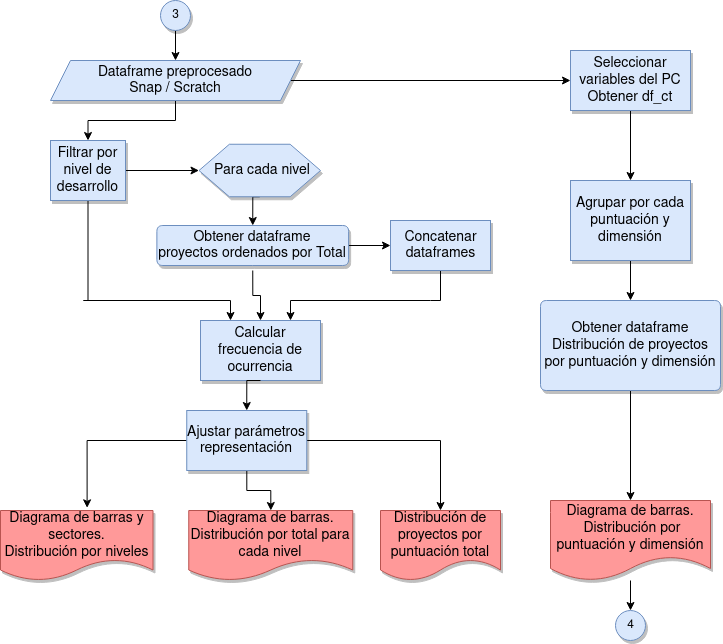
\includegraphics[height=.5\textheight]{img/diseno_distribucion}
    \caption{Diseño de etapa EDA univariante: distribuciones}\label{fig:eda_uni}
\end{figure}

Para continuar indagando en este análisis exploratorio de datos, los proyectos de cada nivel son ordenados y filtrados según la puntuación total conseguida. Al representar los resultados en un diagrama de barras, podemos descubrir tendencias y conocer las puntuaciones más frecuentes en cada nivel.
Se concatenan los dataframes de cada nivel para obtener un diagrama de barras con la frecuencia de ocurrencia de cada puntuación total. Con ello se vislumbra la distribución de los proyectos según su puntuación total, si existen asimetrías hacia las puntuaciones más bajas y las modas de la distribución.

Se instancia un objeto de la clase dataframe escogiendo las siete variables discretas que definen las capacidades del pensamiento computacional consideradas, llamado \texttt{df\_ct}. Se realiza un estudio unidimensional al agrupar los proyectos según la valoración recibida de 0 a 3 en cada dimensión. Se obtiene por iteración el objeto \texttt{df\_score\_ct}, con 4 filas y 7 columnas, gracias al método \texttt{groupby()} de Pandas. Así se pueden comparar las distribuciones de cada habilidad y la dificultad que entraña desarrollarlas, en base al extenso volumen de proyectos analizados. Además de conocer que habilidades resultan más fáciles, también se distingue si las métricas empleadas son consistentes con un grado de complejidad creciente para cada dimensión.

\section{EDA: resumen por métricas estadísticas} 
\label{sec:EDA_estadísticos}

Se llama al método \texttt{describe()} del objeto \texttt{df\_ct} para obtener, de cada variable discreta del pensamiento computacional, su media, su desviación típica, el rango de valores, la posición de sus cuartiles cuando se ordenan los proyectos de menor a mayor puntuación y su mediana, que coincide con el segundo cuartil. La media y la mediana describen cada distribución por el centro de gravedad o la puntuación del proyecto situado en su centro. Con ellas podemos saber qué habilidades consiguen mejores puntuaciones. Con la varianza y la desviación típica se conoce la dispersión de los proyectos con respecto a la media. 

Se representa el diagrama de cajas de las habilidades con la función \texttt{boxplot()}. Nos permite comparar las distribuciones en función de su rango intercuartílico ($IQR=Q_3 - Q_1$), los límites superior e inferior calculados a partir de él y la presencia de \emph{outliers} o valores atípicos. Se analizan en detalle en los apartados~\ref{subsec:estad_pc_Scratch} y~\ref{subsec:estad_pc_Snap}.   

\section{EDA: correlaciones de las dimensiones del PC} 
\label{sec:EDA_corr}

Con el objetivo de establecer el grado de dependencia existente entre la puntuación total con cada una de las variables o habilidades que la conforman, entre estas habilidades entre sí y la evolución de estas asociaciones según aumenta la puntuación total, se calcula el coeficiente de correlación de Pearson, definido en la ecuación~\ref{eq:correlacion}. 

Primero se recurre al método \texttt{corrwith()} del objeto \texttt{df\_ct} para determinar cómo aumenta la puntuación total según se incrementa cada variable del pensamiento computacional. Devuelve un objeto de tipo serie que nos ayuda a identificar qué habilidades presentan menores interdependencias lineales con el total resultante de la agregación de sus valores.

A continuación se obtiene la matriz simétrica con los coeficientes de correlación de Pearson entre cada par de capacidades. Se aplica el método \texttt{corr()} sobre \texttt{df\_ct} y se representa la matriz mediante un mapa de calor que resalta las habilidades con relaciones positivas más fuertes. Así se puede comprobar si las capacidades que conceptualmente se desarrollan juntas, como sincronización y paralelismo o control de flujo y pensamiento lógico, realmente muestran esa dependencia en las poblaciones de  proyectos de Scratch y Snap! analizadas.

\begin{figure}[H]
    \centering
    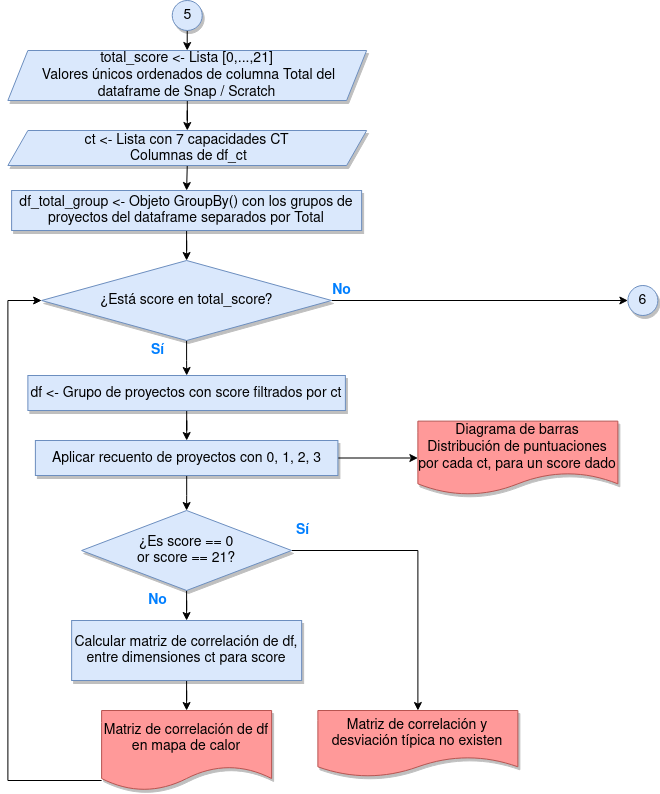
\includegraphics[height=.5\textheight]{img/diagrama_corr2.png}
    \caption{Diagrama de flujo de df\_correlation\_bar\_chart(score, ct)}\label{fig:diagrama_corr}
\end{figure}

Para mostrar las dependencias lineales que se van produciendo según aumenta la complejidad de los proyectos, se sigue el algoritmo representado en el diagrama~\ref{fig:diagrama_corr}. Recibe como parámetros de entrada dos listas, \texttt{total\_score}, con las puntuaciones totales únicas y ordenadas conseguidas por los proyectos, y \texttt{ct}, con las variables o atributos de \texttt{df\_ct}. Se encarga de obtener un dataframe con el grupo de proyectos para cada puntuación total, filtrarlos y devolver la distribución de puntuaciones para cada habilidad. Comprueba que el grupo de proyectos no sea el de las puntuaciones totales extremas, puesto que en ellos la media coincide con la valoración obtenida por cada proyecto para cada dimensión, no existiendo variación conjunta entre cada par de habilidades o covarianza, ni en cada una por separado o desviación típica. Su razón, que es la correlación, tampoco existe. Si la puntuación es válida, calcula y representa la matriz de correlación del grupo. Se repite el proceso para cada puntuación total. 

\section{ML no supervisado: Clustering K-Means}  
\label{sec:k_means diseño}

Al no disponer de una variable de salida u objetivo y contar con una elevada cantidad de proyectos, se aplica un modelo de aprendizaje no supervisado particional, clustering K-Means. Agrupa los proyectos por similitud, extrayendo patrones entre sus características basados en la  distancia al centro de cada grupo. Es preciso conocer a priori el número de grupos o centros (k). Para determinarlo se sigue el diagrama de flujo~\ref{fig:kmeans}. 

Se definen los proyectos como puntos en un espacio métrico de siete dimensiones, que son las características del pensamiento computacional analizadas. Se obtiene un array X con tantas filas como proyectos y tantas columnas como habilidades PC. Se establece un rango de valores de k a probar. Se ejecuta \texttt{KMeans()} para cada valor de k. Tras iteraciones sucesivas en que se asignan los proyectos al centro más cercano y se recalculan las medias aritméticas de los k grupos, que serán los nuevos centroides, el algoritmo converge. Los centros y los proyectos asignados se estabilizan. El algoritmo devuelve la iteración con menor inercia para ese valor de k, siendo la inercia la suma de los cuadrados de la distancia euclídea intra-clúster.

Una vez se tienen los valores de inercia para los distintos valores de k, se busca un compromiso entre un bajo valor de inercia y un número de grupos no muy elevado. Si k es muy elevado, proyectos similares pertenecerán a grupos diferentes, produciéndose granularidad. Su representación gráfica es la curva de Elbow. El valor de k donde se produzca un cambio abrupto de pendiente a partir del cual no disminuya demasiado la inercia será el número de grupos escogido. Si no se distingue con claridad ese punto se recurre a otros métodos de validación interna. Para los proyectos de Snap! he aplicado tres técnicas que utilizan como parámetro las etiquetas que indican a cuál de los k grupos pertenece cada proyecto, tras aplicar K-Means. 

\begin{itemize}
    \item \textbf{Coeficiente de la silueta:} Mide para cada proyecto etiquetado su separación con respecto a los proyectos de los clústeres vecinos relacionándola con la cohesión o distancia a todos los proyectos del mismo clúster, según se muestra en la ecuación~\eqref{eq:silueta}
    \begin{equation}
        SC(x)=\frac {b(x)-a(x)}{max[a(x),b(x)]},\quad\mathit{siendo}\ -1\leq SC \leq1
        \label{eq:silueta}
    \end{equation}   
    \begin{itemize}
        \item \emph{b(x):} Separación o distancia media inter-clúster del proyecto con todos los proyectos del clúster vecino o clúster más próximo.
        \item \emph{a(x):} Cohesión de cada clúster o distancia media intra-clúster del proyecto con todos los proyectos del mismo clúster.
    \end{itemize}
    Si $b(x)\gg a(x)$ indica que el clúster en el que se localiza el proyecto es muy compacto y difiere de los proyectos del grupo más próximo. Si $b(x)= a(x)$, el proyecto se encuentra en la frontera de decisión entre dos grupos. Si $b(x)\ll a(x)$ implica que el proyecto ha sido asignado al grupo incorrecto~\cite{rousseeuv_87}. Utilizando la función de scikit-learn \texttt{silhouette\_score()} obtenemos el promedio de los coeficientes de todos los proyectos para cada uno de los valores de k. Se escoge el valor de k que conlleve una mayor separación entre los grupos, aquel cuyo promedio de los coeficientes de la silueta sea más cercano a 1. 
    \item \textbf{Índice de Davies-Bouldin:} Relación entre la suma de las distancias promedio de los proyectos de cada clúster con el centroide para dos clústeres y la distancia entre los centroides de ambos clústeres. Se calcula para el peor de los casos, cuando los diámetros de los grupos son muy amplios y sus centros están muy juntos, como se ve en la ecuación~\eqref{eq:davies-bouldin}. 
    \begin{equation}
        DB=\frac{1}{k}\sum \limits _{i=1,i\neq j}^{k} max\frac{d(c_i)+d(c_j)}{d(c_i ,c_j)}
    \label{eq:davies-bouldin}
    \end{equation} 
    Nos interesa un valor cercano a 0, que nos indique que no hay similitud entre los clústeres más parecidos de los k grupos. Se llama a la función \texttt{davies\_bouldin\_score()} para cada uno de los valores de k de la secuencia, escogiendo el número de grupos que minimice este índice~\cite{davies1979cluster}.
    \item \textbf{Índice de Calinski-Harabasz:} Es el criterio de relación de varianza, que compara la dispersión entre los grupos con la dispersión intra-clúster, ponderado por el ratio de la ecuación~\eqref{eq:davies-bouldin}, donde N es el número de proyectos y k el número de clústeres.
    \begin{equation}
        CH=\frac{SSB}{SSW}x\frac{N-k}{k-1}
        \label{eq:ch}
    \end{equation} 
    En nuestra búsqueda del k óptimo, nos interesa un valor de pico, que indique que los k grupos son densos y existe una elevada varianza y separación con respecto a otros grupos. Se comparan los distintos índices para cada k, al emplear \texttt{calinski\_harabasz\_score()}.	
\end{itemize}

\begin{figure}[H]
    \centering
    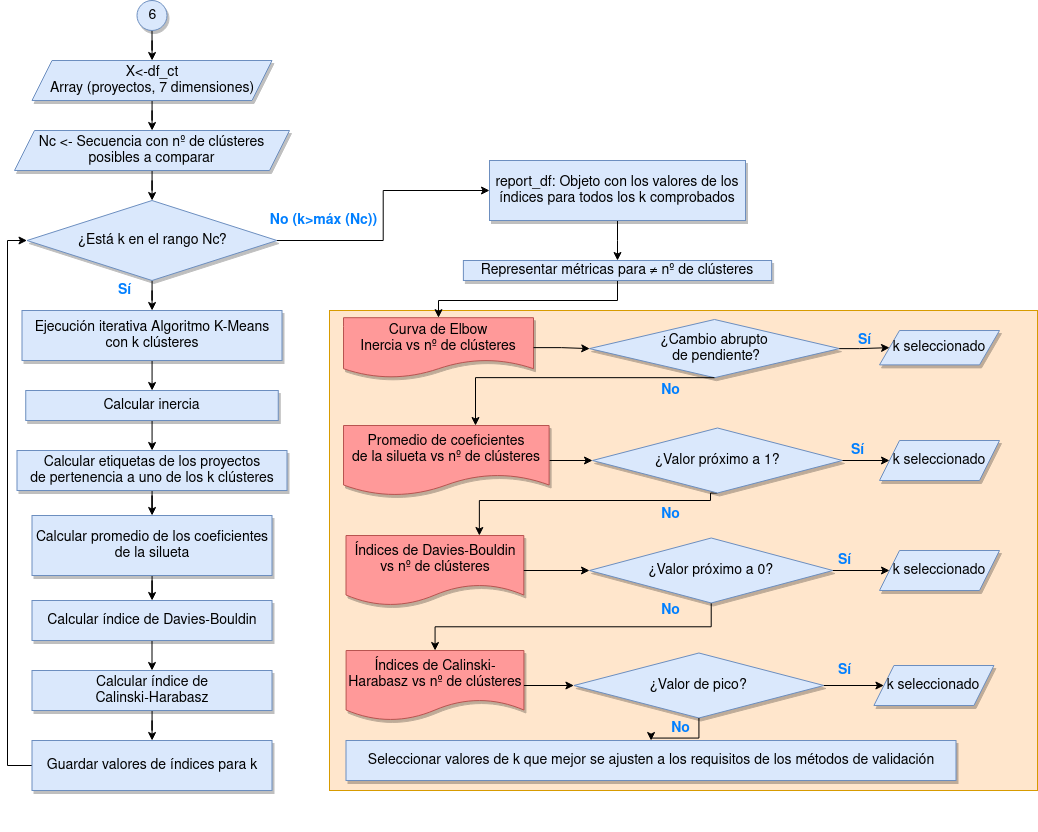
\includegraphics[height=.5\textheight]{img/kmeans_diseno.png}
    \caption{Diagrama de flujo para determinar el número de grupos k para el clustering K-Means.}\label{fig:kmeans}
\end{figure}

A partir de la visualización de estas métricas para los diferentes valores de k, se escoge el número de grupos óptimo, que cumple los requisitos mencionados y resumidos en la figura~\ref{fig:kmeans}. Si no hay un único k donde coincidan los criterios, se prueba el algoritmo K-Means con los posibles valores de k que mejor se adapten a los mismos y se establecen similitudes y diferencias entre los proyectos agrupados con los distintos valores de k.

\section{Rutas de aprendizaje con proyectos representativos}  
\label{sec:rutas_diseño}

Para poder responder a cómo es el proceso de aprendizaje empírico que se manifiesta al analizar las extensas poblaciones de proyectos de Scratch y Snap! se plantea el diagrama~\ref{fig:diagrama_rutas}. 

En este caso no estamos interesados en segmentar los proyectos en k grupos aplicando el algoritmo K-Means directamente. El criterio elegido para su partición es la puntuación total que obtienen. El objeto devuelto por groupby() agrupa los proyectos de nuestro dataset en función de su puntuación total. K-Means toma el grupo de una puntuación con k=1 y se ejecuta iterativamente hasta que el centroide o centro se sitúa en el punto medio que minimiza la suma de las distancias euclídeas de cada proyecto del grupo a este centro. Cuando el algoritmo converge, se calcula cuál es el proyecto más cercano a este centroide, expresado como un vector de características cuyas coordenadas son las 7 dimensiones del pensamiento computacional que mejor caracterizan al grupo. Se repite el proceso para cada grupo definido por su puntuación total.

\begin{figure}
    \centering
    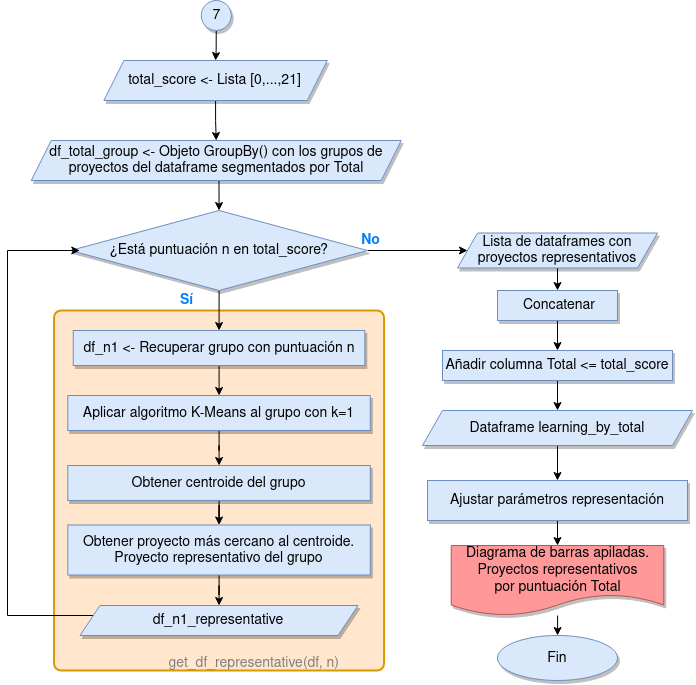
\includegraphics[height=.6\textheight]{img/ruta_de_aprendizajeCaja.png}
    \caption{Diagrama de flujo para la obtención de rutas de aprendizaje}\label{fig:diagrama_rutas}
\end{figure}

Una vez se ha obtenido el proyecto representativo de cada puntuación total, se concatenan los dataframes de una fila, en los que se ha representado cada vector, en una única tabla \texttt{learning\_by\_total}, a la que se añade la variable total. Se representan los prototipos de cada puntuación total, para visualizar la mejora de qué habilidad nos permite pasar a la siguiente puntuación y qué valores recibe cada capacidad en cada nivel de complejidad. Los resultados se recogen en los diagramas de barras~\ref{fig:path_Scratch} y~\ref{fig:path_Snap}.

%%%%%%%%%%%%%%%%%%%%%%%%%%%%%%%%%%%%%%%%%%%%%%%%%%%%%%%%%%%%%%%%%%%%%%%%%%%%%%%%
%%%%%%%%%%%%%%%%%%%%%%%%%%%%%%%%%%%%%%%%%%%%%%%%%%%%%%%%%%%%%%%%%%%%%%%%%%%%%%%%
% EXPERIMENTOS Y VALIDACIÓN %
%%%%%%%%%%%%%%%%%%%%%%%%%%%%%%%%%%%%%%%%%%%%%%%%%%%%%%%%%%%%%%%%%%%%%%%%%%%%%%%%

\cleardoublepage
\chapter{Experimentos y validación}
\label{chap:experimentos}

Tras realizar el proceso de análisis de datos completo con todos los proyectos de Snap!, se cambió la puntuación total en vez de como media, como suma de las puntuaciones obtenidas en cada dimensión y se pasó de 4 a 3 niveles de competencia suprimiendo la categoría sin nivel. De este modo queda más representativo y comparable con los resultados de Scratch.

Además se comprobó que las métricas de la tabla~\ref{table:competence_level_Snap} que definen cada habilidad no estaban bien calibradas. Se quitó la dimensión de diversidad, por no aportar expresividad. El cálculo de las métricas de abstracción y condicionales fue completamente reformulado. Se incluyó la presencia de clones en el código como componente a evaluar en el proyecto de Snap! Por lo tanto, la descomposición del problema en partes más sencillas una vez definido qué es lo relevante para resolverlo, se mide en función del número de scripts y de sprites, la declaración de funciones o bloques personalizados codificados por el desarrollador de Snap! y la instanciación de objetos o personajes. Se tiene en cuenta la complejidad incremental, de manera que para obtener 2 puntos se incluyen 2 cualesquiera de las prácticas mencionadas y para obtener la máxima puntuación deben aparecer las 3. Para condicionales se propuso una metodología equivalente, asignando 1 punto cuando se emplea un if o un if-else o algún operador lógico, 2 puntos si se usan dos de estas estructuras selectivas y 3 puntos cuando se aplican todas de manera apropiada.

Para paralelismo, sincronización, control de flujo e interactividad con el usuario, se mapearon los elementos inherentes a cada habilidad de manera diferente, haciendo que las métricas fueran discriminantes y presentaran una dificultad creciente. Mediante ensayo y error se fueron reajustando hasta obtener unas distribuciones y rutas de aprendizaje válidas y con mayor sentido tanto a nivel teórico como práctico. Se resumen los cambios aplicados en la tabla~\ref{table:modif_level_Snap}.

\begin{table}[H]
    \centering
    \resizebox{15cm}{!}{
    \begin{tabular}{|m{3.5cm}|m{5cm}|m{5cm}|m{5cm}|}
       \rowcolor[HTML]{CBCEFB}
       \textbf{Dimensión del PC} & \textbf{Básico} - 1 punto & \textbf{Intermedio} - 2 puntos & \textbf{Avanzado} - 3 puntos\\ \hline
       \textbf{Abstracción} & Más de un objeto con más de un script o definición de bloques propios o clon creado. & Contiene 2 tipos: más de un objeto con varios scripts y/o definición de bloques propios y/o clon creado. & Contiene los 3 tipos de abstracción considerados. \\ \hline
       \textbf{Paralelismo} & Un objeto ejecuta 2 o más scripts ante los eventos: bandera verde o pulsar una tecla. & 2 objetos ejecutan 1 o más scripts a la vez ante los eventos: bandera verde o pulsar una tecla. & 1 o más objetos ejecutan 2 scripts cuando reciben un mensaje, cuando se cumple una condición o usan clones. \\ \hline % No es el máx
       \textbf{Condicionales} & 1 estructura selectiva: if o if-else u operaciones lógicas. & 2 estructuras selectivas: if, if - else u operaciones lógicas. & Se utilizan las 3 estructuras condicionales. \\ \hline 
       \textbf{Sincronización} & Esperar. &  Enviar, cuando reciba mensaje, parar todos, parar script. & Preguntar a un objeto por, esperar hasta, enviar y esperar, cuando se cumple condición o empiece como clon. \\ \hline % dato de cualquier tipo
       \textbf{Control de flujo} & Secuencia de bloques. & Repetir n veces, por siempre o bucle for. & Repetir hasta. \\ \hline
       \textbf{Interactividad con el usuario} & Eventos: bandera verde o pulsar una tecla. Sensores:   
       tecla u objeto pulsado. & Preguntar al usuario y obtener respuesta.
       Eventos con el ratón sobre el objeto.
       & Detección de colisiones, acciones en audio y vídeo. \\ \hline
       \textbf{Representación de los datos} & Modificadores de atributos de los objetos. & Funciones con variables. & Funciones con listas. \\ \hline
    \end{tabular}}
    \caption{Ajuste de métricas en cada dimensión del PC en Dr. Snap!}
    \label{table:modif_level_Snap}
\end{table}


%%%%%%%%%%%%%%%%%%%%%%%%%%%%%%%%%%%%%%%%%%%%%%%%%%%%%%%%%%%%%%%%%%%%%%%%%%%%%%%%
%%%%%%%%%%%%%%%%%%%%%%%%%%%%%%%%%%%%%%%%%%%%%%%%%%%%%%%%%%%%%%%%%%%%%%%%%%%%%%%%
% RESULTADOS %
%%%%%%%%%%%%%%%%%%%%%%%%%%%%%%%%%%%%%%%%%%%%%%%%%%%%%%%%%%%%%%%%%%%%%%%%%%%%%%%%

\cleardoublepage
\chapter{Resultados}
\label{chap:resultados}

Se filtran y agrupan los datos para realizar cálculos estadísticos y matemáticos que nos permitan descubrir y visualizar información contenida en los mismos empleando las bibliotecas de pandas, matplotlib y seaborn para ver qué habilidades del PC se desarrollan con mayor facilidad, cuáles resultan más complejas, ver si existen relaciones entre ellas, cuál es el camino de aprendizaje empírico demostrado a partir de un volumen de proyectos suficientemente amplio y representativo del conjunto de proyectos de Scratch y Snap! Comparándolos se puede ver si los desarrolladores de los proyectos siguen las mismas pautas o por el contrario tienen más facilidad para desarrollar un conjunto de capacidades distintas, puesto que se parte de la base de que los programadores de proyectos de Snap! ya tienen ciertos conocimientos tanto en programación como en el proceso cognitivo que la sustenta.

\section{Análisis de datos de proyectos de Scratch} 
\label{sec:result_scratch}

\subsection{Extracción y limpieza de datos}
\label{subsec:clean_data_Scratch}

A partir del proceso de extracción y recolección de datos de los 269.844 proyectos de Scratch desde el servidor de Dr. Scratch en un fichero llamado \emph{results.csv}, se obtiene un dataset de partida con tantas observaciones como proyectos y 11 variables, atributos o características. Estas variables incluyen el nombre único del proyecto de Scratch, las puntuaciones discretas en el rango [0, 3] conseguidas para cada una de las 7 dimensiones del pensamiento computacional, la suma y el valor medio de las mismas, asignadas a las características total y media y el nivel básico, desarrollador o profesional. En la figura~\ref{fig:df_Scratch} se muestra la estructura de datos bidimensional de los diez primeros proyectos y los valores en bruto de los datos para las características mencionadas. 

\begin{figure}[H]
    \centering
    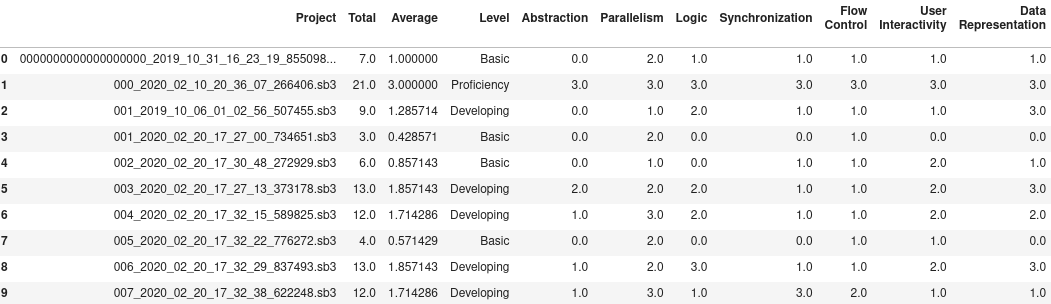
\includegraphics[width=1.0\textwidth]{img/df_origen_Scratch.png}
    \caption{Dataframe de los proyectos de Scratch obtenido al cargar \emph{results.csv}}\label{fig:df_Scratch}
\end{figure}

Se comprueba que no existen proyectos de Scratch duplicados y se eliminan 2, cuyas variables no tienen valores asignados. Como resultado se obtiene un dataset con 269.842 proyectos. Se ajustan los tipos de las variables a discretas para las puntuaciones de cada dimensión y para la total, y de tipo categórico ordinal para los tres niveles que pueden alcanzar los proyectos de Scratch en función de su puntuación total: \emph{ básico o ``basic''} de 0 a 7 puntos, \emph{desarrollador o ``developing''} de 8 a 14 puntos y \emph{profesional o ``proficiency''} de 15 a 21 puntos. % Se eliminan 2 de ellos

\subsection{Análisis de los proyectos de Scratch por nivel o categoría asignada y puntuación total. Distribución de frecuencias}
\label{subsec:frec_nivel}

Tras el preprocesamiento y limpieza de datos, se continúa con el análisis exploratorio de datos, en el que se responde a ¿cómo es la distribución de los proyectos de Scratch por nivel? 

En los diagramas de barras y de sectores de la figura~\ref{fig:level_Scratch} se clasifican los proyectos de Scratch según la etapa de desarrollo en que se encuentren. La categoría ``\emph{basic}'' es la más frecuente pues agrupa 131.007 proyectos que constituyen un 48,55\% del conjunto total. El siguiente nivel más frecuente es el intermedio o ``\emph{developing}'' con un 38,59\% del dataset completo, que se corresponde con 104.142 proyectos. Únicamente 34.693 proyectos de Scratch, un 12,86\% del total, alcanzan el nivel avanzado o ``\emph{proficiency}''. Aproximadamente la mitad de los proyectos de Scratch analizados son muy sencillos y no consiguen puntuar por encima de los 7 puntos totales. En contraste solo un 12,86\% demuestran un dominio del pensamiento computacional superior a los 14 puntos.

\begin{figure}[H]
    \centering
    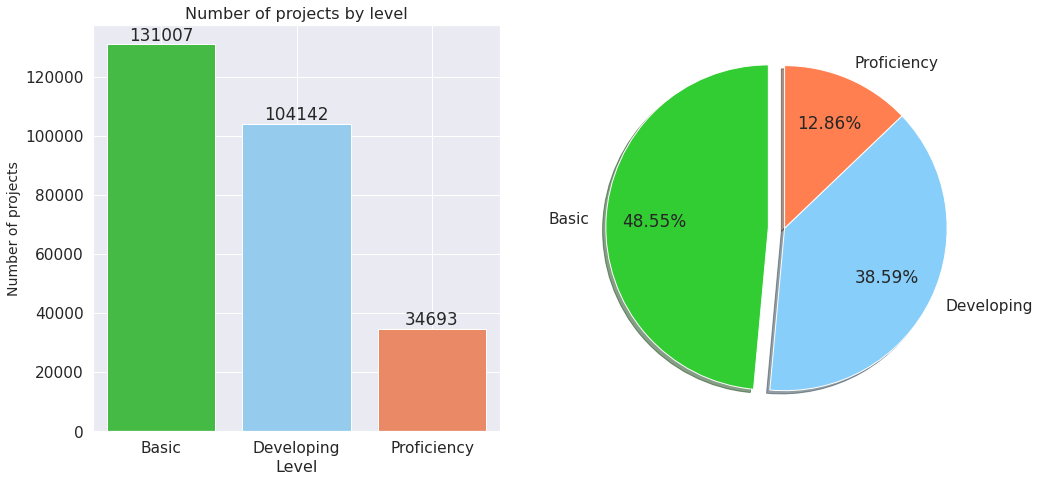
\includegraphics[width=1.0\textwidth]{img/freq_level_Scratch.png}
    \caption{Distribución de proyectos de Scratch por nivel asignado}\label{fig:level_Scratch}
\end{figure}

¿Cómo se distribuyen los proyectos de Scratch entre las distintas puntuaciones asignadas a cada nivel?

Para la categoría \emph{basic} representada en la figura~\ref{fig:basic} se aprecia una tendencia ascendente en la puntuación conseguida, con un máximo en los 7 puntos. Si bien es importante remarcar que 16.289 proyectos no consiguen puntuar por estar incompletos.

Sin embargo en la categoría intermedia o \emph{developing}, se sigue una tendencia descendente, como se observa en la figura~\ref{fig:developing}.

En la categoría de nivel avanzado o \emph{proficiency} se continúa con una tendencia descendente hasta los 18 puntos. Se eleva a 5.570 la cantidad de proyectos con 19 puntos, para disminuir notablemente en los 21 puntos totales (véase figura~\ref{fig:proficiency}). Únicamente 180 proyectos obtienen la calificación máxima en cada una de las siete dimensiones del pensamiento computacional. 

\begin{figure}[H]
    \centering
    \begin{subfigure}[h]{.75\textwidth} 
        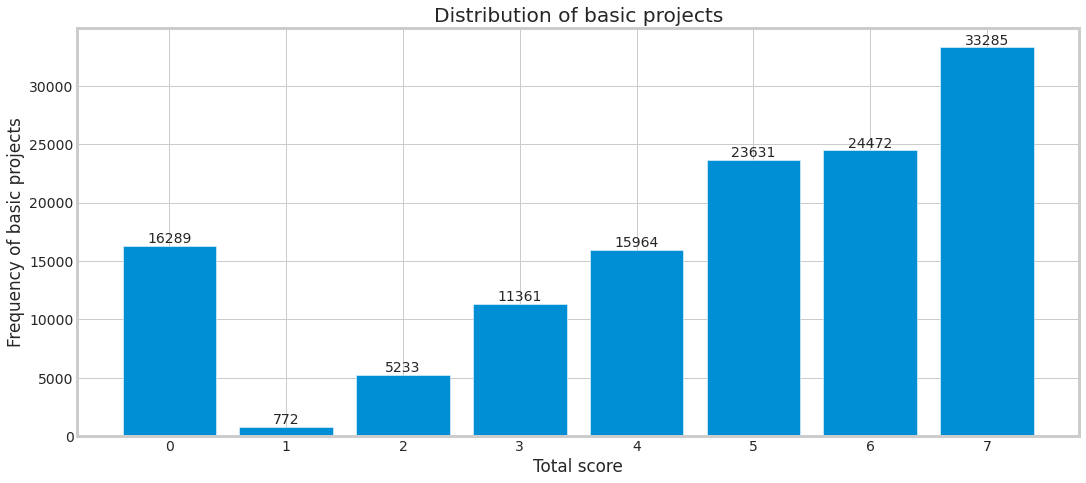
\includegraphics[width=\textwidth]{img/basic_Scratch}
        \caption{Nivel básico}
        \label{fig:basic}
    \end{subfigure}       
    \begin{subfigure}[h]{.75\textwidth} 
        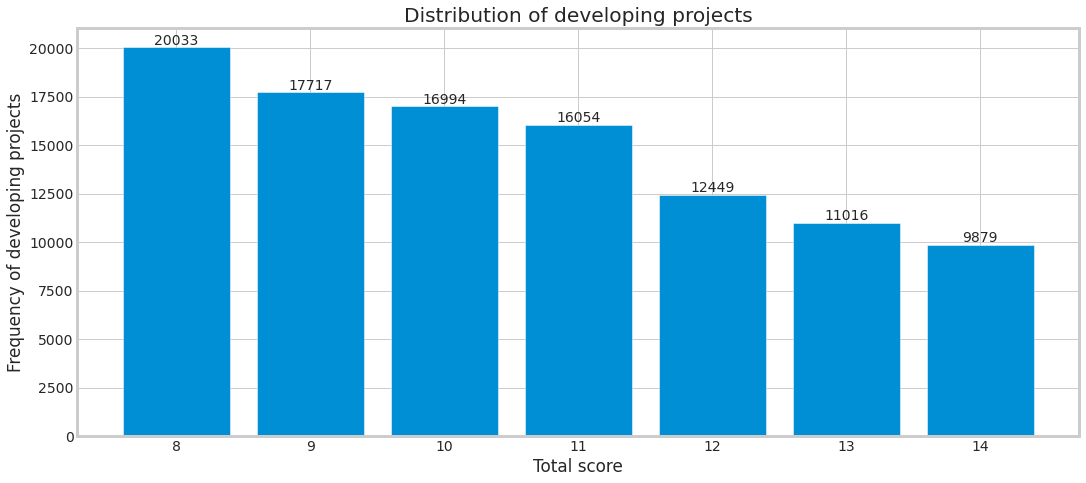
\includegraphics[width=\textwidth]{img/developing_Scratch}
        \caption{Nivel intermedio}
        \label{fig:developing}
    \end{subfigure}
    \begin{subfigure}[h]{.75\textwidth} 
        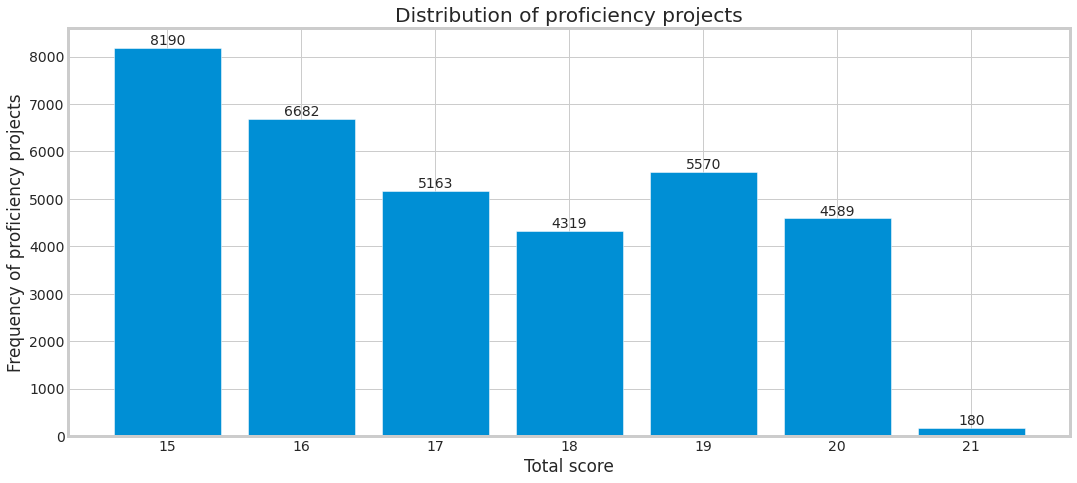
\includegraphics[width=\textwidth]{img/proficiency_Scratch}
        \caption{Nivel avanzado}
        \label{fig:proficiency}
    \end{subfigure}
    \caption{Distribución de proyectos de Scratch por puntuaciones asignadas a cada nivel}
\end{figure}

En la tabla~\ref{table:mean_Scratch} se indican las medidas de tendencia central y de dispersión para cada nivel. En el nivel \emph{basic}, al ser la media menor que la mediana, la distribución tiene una asimetría negativa o hacia la izquierda. En los niveles \emph{developing} y \emph{proficiency} la asimetría es positiva o hacia la derecha, puesto que la media supera a la mediana, aunque en los gráficos de distribución no es tan evidente. La dispersión de los valores de la puntuación con respecto a la media disminuye según aumenta el nivel, aunque se mantienen valores elevados de desviación típica para todos ellos, implicando que la mediana será más representativa que la media.

\begin{table}[htbp]
 \begin{center}
  \begin{tabular}{|c|c|c|c|c|}
    \hline
     \textbf{Nivel} & \textbf{Media} & \textbf{Mediana} & \textbf{Varianza} & \textbf{Desviación típica} \\ \hline
    \textbf{Basic} & 4.634554 & 5 & 5.100514 & 2.258432 \\ \hline
    \textbf{Developing} & 10.535164 & 10 & 3.755300 &  1.937860 \\ \hline
    \textbf{Proficiency} & 17.198426 & 17 & 3.137785 &  1.771379 \\ \hline
  \end{tabular}
  \caption{Medidas de tendencia central y dispersión para cada nivel de Scratch.}
  \label{table:mean_Scratch}
 \end{center}
\end{table}

¿Cómo se distribuyen los proyectos de Scratch según la puntuación total?

Cómo se percibe en la figura~\ref{fig:total_Scratch}, se produce una elevada concentración de proyectos entre los 4 y los 11 puntos, con un máximo en los 7 puntos. La cantidad de proyectos que consiguen cada puntuación crece rápidamente hasta esta puntuación más frecuente o moda. A partir de la misma disminuye de manera más suave, obteniendo una cola que se extiende hacia la derecha según la valoración total del proyecto toma los valores más altos.

\begin{figure}[H]
    \centering
    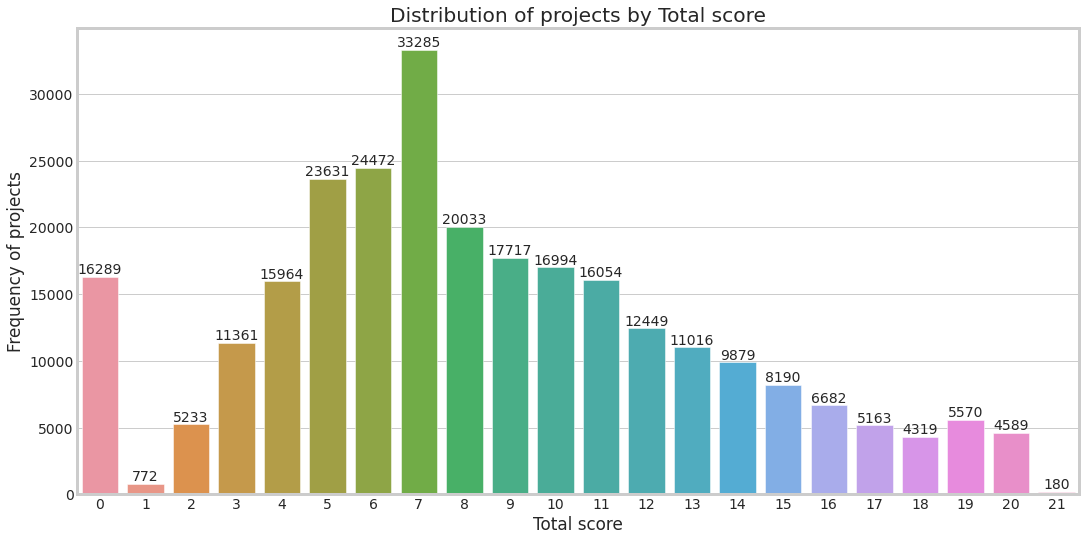
\includegraphics[width=.9
    \textwidth]{img/frequency_total_score_Scratch.png}
    \caption{Distribución de proyectos de Scratch por puntuación total}\label{fig:total_Scratch}
\end{figure}

Parece razonable que aproximadamente la mitad de los proyectos se encuentren en un nivel básico con puntuaciones totales bajas, puesto que el público objetivo son alumnos que se inician en la programación y en el desarrollo de su pensamiento computacional con proyectos sencillos codificados en Scratch. La finalidad es que los alumnos incrementen la  complejidad de sus proyectos, al verse motivados por la realimentación que proporciona Dr. Scratch para mejorar en cada dimensión del pensamiento computacional y evitar malos hábitos al programar. La cantidad de proyectos que superen el umbral de los 7 puntos debería incrementarse para ascender a las categorías superiores. No obstante resulta complicado implementar proyectos que contengan todos los conceptos y prácticas computacionales de mayor valoración en cada dimensión.

\subsection{Frecuencia de los proyectos de Scratch por áreas del pensamiento computacional}
\label{subsec:frec_pc_Scratch}

¿Cuál es la distribución de la puntuación en cada dimensión?

Se filtran y agrupan los proyectos según las métricas establecidas en Dr. Scratch para cada destreza del pensamiento computacional en la tabla~\ref{table:competence_level_Scratch}.

\begin{figure}[H]
    \centering      
    \begin{subfigure}[h]{1\textwidth} 
        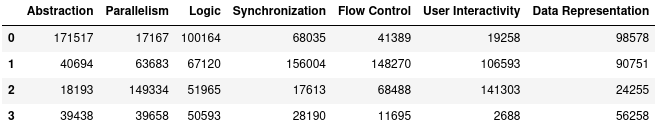
\includegraphics[width=\textwidth]{img/df_PC_Scratch.png}
        \caption{Dataframe con la cantidad de proyectos por puntuación y dimensión del PC}
        \label{fig:df_PC_Scratch}
    \end{subfigure}
    \begin{subfigure}[h]{1\textwidth} 
        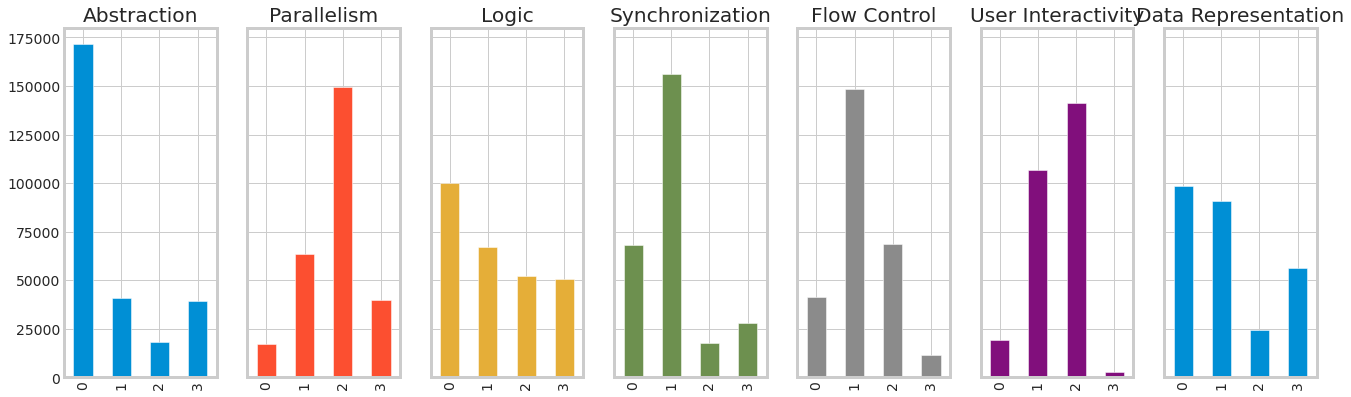
\includegraphics[width=\textwidth]{img/distribution_PC.png}
        \caption{Diagrama de barras con la cantidad de proyectos por puntuación y dimensión del PC}
        \label{fig:barras_PC_Scratch}
    \end{subfigure} 
\caption{Distribución de proyectos de Scratch por puntuación para cada dimensión del PC}
\end{figure}

\begin{itemize}    
    \item \textbf{Abstracción}: Es la capacidad menos desarrollada. Se utiliza más de un script y más de un personaje u objeto en 40.694 proyectos, estando evaluados con 1 punto. Los 3 puntos asignados por el uso de clones tienen una frecuencia absoluta similar, con 39.438 proyectos. Únicamente 18.193 proyectos tienen bloques o funciones definidas por el programador. Un total de 171.517 proyectos carecen de estos elementos vinculados con la descomposición del problema en partes más sencillas que puedan ser reutilizadas tras extraer lo relevante de cada parte, descubrir patrones y generalizar.    
    \item \textbf{Paralelismo}: La puntuación de 2 puntos destaca sobre las demás, con 149.334 proyectos que cuentan con flujos de código que se ejecutan simultáneamente al pulsar sobre una tecla o sobre un objeto.    
    \item \textbf{Pensamiento lógico}: En 100.164 proyectos del dataset no se emplean estructuras condicionales que seleccionen las instrucciones a realizar en función de que se cumpla una condición. Un conjunto de 67.120 proyectos cuentan con al menos un if, 51.965 con un if-else y 50.593 emplean operadores lógicos, disminuyendo la frecuencia según aumenta la complejidad.    
    \item \textbf{Sincronización}: En 156.004 proyectos se emplean bloques de espera para establecer el orden en que los programas de un proyecto se ejecutan, haciendo que interactúen entre sí, consiguiendo por ello 1 punto. Elementos como el intercambio de mensajes o establecer eventos de parada solo se utilizan en 17.613 proyectos evaluados con 2 puntos. Aumenta la frecuencia de los que son valorados con 3 puntos por emplear eventos como el cambio de escenario o el resultado de la ejecución de otro programa para que se continúe con la ejecución de las sentencias sujetas a que se produzcan estos eventos.    
    \item \textbf{Control de flujo}: En más de la mitad de los proyectos, en concreto en 148.270, se demuestran nociones algorítmicas al secuenciar las instrucciones de manera concreta y precisa. Por ello obtienen un punto. La distribución se reduce linealmente, de modo que 68.488 proyectos emplean bucles infinitos o que iteran un número concreto de veces. Las estructuras iterativas sujetas a condiciones están presentes en 11.695 proyectos, que reciben 3 puntos.  
    \item \textbf{Interactividad con el usuario}: Se evalúa la gestión de las acciones que el usuario realiza sobre el programa cuando mueve el ratón, pulsa sobre los objetos, presiona teclas del teclado o responde a preguntas con 2 puntos, alcanzados en 141.303 proyectos. La siguiente valoración más frecuente es 1 punto, con 106.593 proyectos que solo cuentan con la bandera verde como elemento interactivo que desencadena la ejecución de los programas.    
    \item \textbf{Representación de la información}: Se modifican los atributos de los objetos o personajes en 90.751 proyectos, que obtienen un punto. Llama la atención la escasez de proyectos que consiguen 2 puntos por inicializar y modificar variables para almacenar los datos que requieren los programas, frente a los 56.258 que utilizan listas y sus métodos, siendo calificados con la máxima puntuación.     
\end{itemize}

\subsection{Análisis estadístico general de las dimensiones del pensamiento \\computacional con Scratch}
\label{subsec:estad_pc_Scratch}

Se complementa el análisis univariante calculando los estadísticos descriptivos más básicos para cada capacidad que se muestran en la figura~\ref{fig:describe_Scratch}. A partir del valor medio y de la medida de posición del segundo cuartil, que coincide con la mediana, se infiere que las habilidades más desarrolladas son paralelismo e interactividad con el usuario, mientras que abstracción es la que resulta más compleja. Su dispersión en torno a la media es una de las más altas, junto a la que se produce en representación de los datos y pensamiento lógico. El 75\% de los proyectos son valorados con 0 o 1 puntos en abstracción y sincronización, mientras que para el resto de dimensiones algunos de ellos alcanzan los 2 puntos. 

\begin{figure}[H]
    \centering
    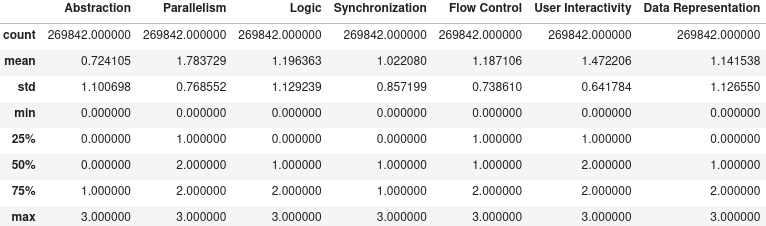
\includegraphics[width=1\textwidth]{img/describe_Scratch.png}
    \caption{Media, desviación estándar y cuartiles de cada habilidad del PC en Scratch}
    \label{fig:describe_Scratch}
\end{figure}

A continuación se representa en la figura~\ref{fig:cajas_Scratch} la concentración de las puntuaciones de cada habilidad del PC en base a la mediana y a los cuartiles y se comprueba si existen valores atípicos.

\begin{figure}[H]
    \centering
    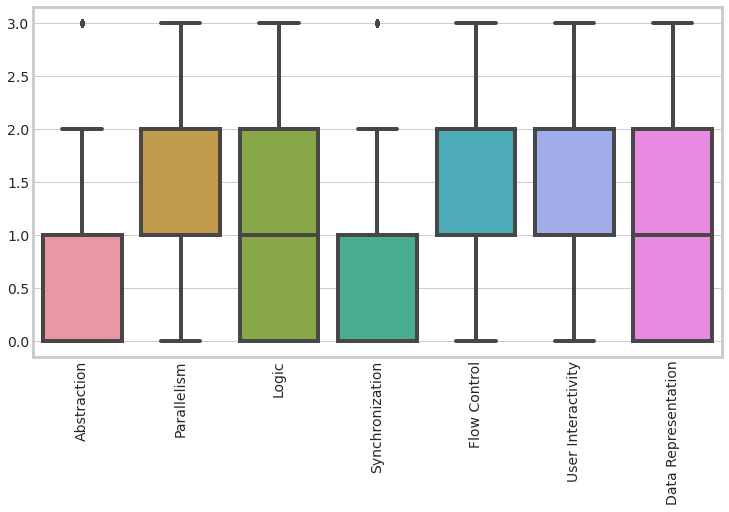
\includegraphics[width=0.7\textwidth]{img/diag_cajas_Scratch2.png}
    \caption{Diagrama de cajas de cada dimensión del PC en Scratch}
    \label{fig:cajas_Scratch}
\end{figure}

\begin{itemize}
    \item \textbf{Abstracción y sincronización}: Al ordenar los proyectos de menor a mayor puntuación más de la mitad no puntúan en abstracción. Por lo tanto el primer cuartil $(Q_1)$ y la mediana están situados en 0. En el tercer cuartil $(Q_3)$ algunos proyectos consiguen 1 punto. En sincronización la mediana coincide con el tercer cuartil en 1 punto. En ambos el 75\% de los proyectos están entre 0 y 1 puntos, el límite superior se localiza en los 2 puntos y los proyectos con 3 puntos serían \emph{outliers} o valores atípicos, pero válidos en este estudio, ya que hay más proyectos con 3 puntos que con 2 puntos, como se veía en la  figura~\ref{fig:df_PC_Scratch}.
    \item \textbf{Paralelismo, interactividad con el usuario y control de flujo}: Sus diagramas de cajas son similares y las distribuciones son más simétricas. Los proyectos alcanzan 1 punto en el primer cuartil y 2 puntos en el tercer cuartil. La mediana de paralelismo e interactividad con el usuario coincide con el tercer cuartil y se corresponde con los 2 puntos. En cambio, para control de flujo la mediana coincide con el primer cuartil en 1 punto. El límite superior para las tres está en 3 puntos. Todo ello indica que las puntuaciones están más concentradas en 1 y 2 puntos, con mayor cantidad de proyectos en el cuartil que coincide con la mediana.
    \item\textbf{Pensamiento lógico y representación de los datos}: También siguen una dispersión similar, con un rango intercuartil de 0 a 2 puntos y la mediana en 1 punto. Sus valores están más dispersos que en las otras dimensiones. El límite superior está en 3 puntos. 
\end{itemize}

Siguiendo con el análisis exploratorio de datos o EDA se calculan los coeficientes de correlación de Pearson existentes entre la puntuación total y las distintas habilidades, para determinar si existe una dependencia lineal perfecta o próxima a 1.


\begin{table}[htbp]
 \begin{center}
 \resizebox{15cm}{!} {
    \begin{tabular}{|c|c|c|c|c|c|c|c|}
    \hline
    \textbf{Correlación} & \textbf{Abstracción} & \textbf{Paralelismo} & \textbf{Lógica} & \textbf{Sincronización} & \textbf{Control de flujo} & \textbf{\begin{tabular}[c]{@{}c@{}}Interactividad\\ con el usuario\end{tabular}} & \textbf{\begin{tabular}[c]{@{}c@{}}Representación\\ de los datos\end{tabular}} \\
    \hline
    \textbf{Total} & 0.772359 & 0.720550 &  0.787795 & 0.753190 & 0.772396 & 0.609517 &  0.786001 \\ 
    \hline
    \end{tabular} }
    \caption{Correlación de la puntuación total con cada dimensión del PC en Scratch}
    \label{table:corr_total_Scratch}
 \end{center}
\end{table}

De la tabla~\ref{table:corr_total_Scratch} se deduce que las correlaciones son directas y fuertes entre la puntuación total y cada dimensión del pensamiento computacional, al ser superiores a $0,7$,
salvo en interactividad con el usuario, que sería la habilidad que menos aporta a la puntuación total y la que más información contiene. Cuando aumenta la puntuación de interactividad se incrementa la puntuación total en menor medida que si crecen las valoraciones de las otras dimensiones.
    
El siguiente paso es indagar si existen relaciones entre las dimensiones del pensamiento computacional o si por el contrario son todas independientes linealmente entre sí. Para ello se realiza un análisis multivariante, calculando la correlación de Pearson para cada par de características o dimensiones.

\begin{figure}[H]
    \centering
    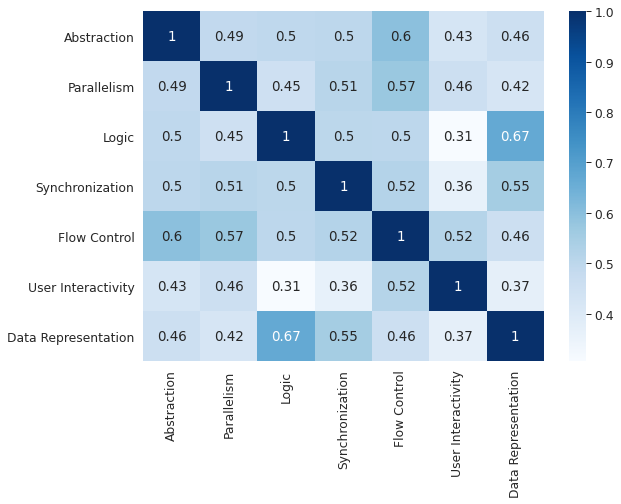
\includegraphics[width=.7\textwidth]{img/corr_Scratch.png}
    \caption{Matriz de correlación de Pearson de las dimensiones del PC.}\label{fig:corr_Scratch}
\end{figure}

Se producen correlaciones positivas débiles y moderadas entre cada par de dimensiones. Las más bajas ocurren entre interactividad con el usuario con cada una de las siguientes: lógica, sincronización y representación de la información. Existe escasa dependencia entre implementar código que se encargue de las acciones que realice el usuario sobre el programa con determinar las sentencias que se ejecutan en función de condiciones, con la organización de la ejecución de los distintos programas de manera que interactúen entre sí y con la declaración y la modificación de los datos sobre los que se opera en los programas.

Los mayores coeficientes de correlación, que se corresponden con una correlación positiva moderada, se obtienen entre:

\begin{itemize}
    \item \textbf{Lógica y representación de los datos}: Cuando se codifican estructuras algorítmicas selectivas, planteando las condiciones que determinan por dónde continúa el flujo del programa, también aumenta la habilidad para definir y manipular los datos de variables, listas y atributos que necesitan los personajes y programas para su ejecución.
    \item \textbf{Abstracción y control de flujo}: La destreza mostrada al descomponer en partes el problema a resolver con funciones y procedimientos encargados de tareas concretas e instanciando objetos o clones cuando se requiera que hagan las mismas instrucciones, guarda relación con las nociones algorítmicas demostradas en cada una de esas partes ya sea secuenciando instrucciones o empleando bucles.
    \item \textbf{Paralelismo y control de flujo}: La capacidad de dividir el problema en programas que son ejecutados a la vez por uno o varios personajes depende linealmente de que los algoritmos que sustentan dichos programas estén definidos de manera precisa y ordenada y utilicen bucles cuando sea recomendable.
    \item \textbf{Sincronización y representación de los datos}: Establecer el orden en que se ejecutan los distintos programas para que interactúen entre sí se relaciona con declarar y modificar las variables, listas y atributos que contienen los datos requeridos en todos ellos.
\end{itemize}


\subsection{Frecuencias y correlaciones de las dimensiones del PC en función de la puntuación total para proyectos de Scratch}
\label{subsec:corr_21_Scratch}

Se profundiza en el análisis multivariante comprobando las dependencias lineales entre cada par de dimensiones del pensamiento computacional según aumenta la puntuación total. Para ello se observa la evolución de la matriz de correlación de Pearson y de las distribuciones de puntuación en cada dimensión. El objetivo es tratar de esclarecer cuáles son las dimensiones que se desarrollan antes, qué puntuaciones se les van asignando y qué relaciones se establecen entre ellas según aumenta la complejidad de los proyectos, determinada por la puntuación total.

En los casos extremos, cuando la puntuación total es de 0 y 21, todas las dimensiones tienen asignadas las mismas puntuaciones en cada proyecto, 0 y 3 respectivamente. No hay dispersión con respecto a la media, tanto al tomar cada variable o dimensión por separado como al analizar la variación conjunta de cada par de variables. Por lo tanto la covarianza y la raíz de la varianza o desviación típica son nulas y su razón, que conforma el coeficiente de correlación, indeterminada (véase la ecuación~\eqref{eq:correlacion}). 

\begin{equation}
   \rho_{xy} = \dfrac{Cov(X,Y)}{\sigma_{x}\sigma_{y}} = \dfrac{\sum_{i=1}^{n} (x_i - \overline{x})(y_i - \overline{y})}{\sqrt{\sum_{i=1}^{n} (x_i - \overline{x})^{2}}\sqrt{\sum_{i=1}^{n} (y_i - \overline{y})^{2}}},  siendo: -1<\rho_{xy}<1
   \label{eq:correlacion}
\end{equation}   

Se prosigue con el desglose de las puntuaciones conseguidas en cada habilidad para cada puntuación total, según progresa de 1 a 20 y se analizan las dependencias que surgen entre ellas. 
Se visualizan y analizan en detalle en el anexo~\ref{append_scratch}. Se expone a continuación lo más relevante.

%%%% Resumen
Para las puntuaciones más bajas existe una interdependencia moderada en sentido negativo entre abstracción y paralelismo, que se  mantiene hasta los 12 puntos, en los que abstracción incrementa su puntuación más frecuente de 0 a 1 punto, por la descomposición del problema en scripts encargados de tareas concretas. El aumento en la cantidad de proyectos que obtienen 3 puntos en abstracción provoca que cambie el sentido de la correlación, de manera que aumenta la ejecución simultánea de varios scripts ante la ocurrencia de eventos. El grado de dependencia se aproxima a 1 según asciende la puntuación total a partir de los 16 puntos totales.

Además se producen dependencias lineales directas casi perfectas entre abstracción y representación de los datos desde los 13 puntos. La declaración y modificación de los datos contenidos en atributos de los objetos, variables y listas permite generalizar y declarar funciones propias, así como crear clones dinámicamente.

Por su parte, paralelismo comienza a puntuar desde los 2 puntos totales y también depende linealmente de lógica, cuando predomina el uso de estructuras selectivas if-else, a partir de los 10 puntos totales. Esta fuerte correlación  entre paralelismo y lógica persiste hasta que ambas alcanzan su máxima puntuación en los niveles más altos de complejidad global.

Por otro lado, resulta llamativo que interactividad con el usuario sea la primera habilidad en manifestarse y la última en completarse, y que mantenga dependencias lineales con control de flujo desde los 10 puntos totales y con paralelismo hasta los 15 puntos totales. No obstante, con paralelismo comparte métricas similares, puesto que se ejecutan varios programas a la vez al pulsar sobre objetos, teclas o la bandera verde, que son acciones puntuadas con 1 y 2 en interactividad con el usuario. 
%%%%


\subsection{Aprendizaje no supervisado: clustering K-Means en proyectos de Scratch}
\label{subsec:kmeans_Scratch}

Se utiliza este algoritmo de aprendizaje no supervisado, para dividir los 269.842 proyectos de Scratch en subconjuntos no solapados o particiones. Se obtienen grupos de manera que los proyectos dentro de un clúster son muy similares, y totalmente distintos a los proyectos que pertenecen a otros grupos. La semejanza o diferencia se mide en función de la distancia euclídea a un centroide del clúster, que a partir de cierto número de iteraciones, se colocará en el centro del clúster. K-Means trata de minimizar las distancias intra-partición y maximiza las distancias inter-partición.

La entrada al algoritmo es un array de vectores con tantas filas como observaciones o proyectos de Scratch y cuyas componentes son las características o dimensiones del pensamiento computacional. Como cada proyecto queda representado por un punto en un espacio de 7 dimensiones cuyas coordenadas son los valores de las puntuaciones asignadas a cada habilidad, al aplicar el algoritmo K-Means, y minimizarse las distancias al punto medio o centroide de cada clúster, la cohesión del grupo determina relaciones y patrones entre las habilidades difícilmente identificables de otro modo, como en el análisis previo de las correlaciones. 

Para aplicar K-Means es necesario conocer a priori el valor de k, el número de grupos o centroides. Una de las técnicas más extendidas para estimarlo es la curva de Elbow. Se itera sobre un conjunto de posibles valores de k buscando un cambio abrupto en la inercia, de forma que un aumento en el valor de k no suponga una disminución significativa en dicha inercia. La inercia se define como la suma de las distancias euclídeas de cada punto con respecto al centroide o centro del clúster al que pertenece, como se indica en la ecuación~\eqref{eq:inercia}.

\begin{equation}
    Inercia=WCSS=\sum \limits _{i=0}^{N} \|{x_i-c_i\|^2}
    \label{eq:inercia}
\end{equation}

\begin{figure}
    \centering
    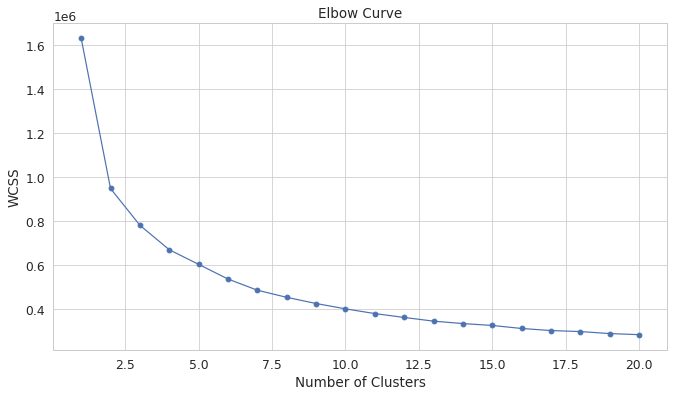
\includegraphics[width=.7\textwidth]{img/elbow_Scratch}
    \caption{Curva de Elbow}
    \label{fig:elbow_Scratch}
\end{figure}

La curva de Elbow de la figura~\ref{fig:elbow_Scratch} comienza a suavizarse a partir de k=3. Se entrena el algoritmo con este valor de k. El algoritmo coloca 3 centroides de manera aleatoria y tras varias iteraciones en que se asigna cada proyecto al centroide más cercano y se recalcula la posición de este centro en función de la media de los proyectos pertenecientes al grupo, llega un momento en que el algoritmo converge. Los centroides no cambian de posición porque no se modifican los proyectos pertenecientes a cada grupo o porque se ha alcanzado el número máximo de iteraciones. Los proyectos son etiquetados según el clúster en el que están incluidos. Cada clúster queda descrito por el proyecto más cercano a su centroide o proyecto representativo.

En el artículo~\cite{moreno17:_paths} se establece un itinerario de aprendizaje en tres pasos, de complejidad incremental, basado en los proyectos representativos o prototipos de los 3 clústeres obtenidos de una muestra de 250 proyectos tomadas del repositorio de Scratch. Se propuso comparar esos prototipos con los proyectos representativos de los 3 clústeres conseguidos en nuestro dataset.  

\begin{table}[H]
    \begin{subtable}[h]{0.49\textwidth}
        \centering
        \begin{tabular}{lrrr}
            {} & \multicolumn{3}{c}{\cellcolor[HTML]{FFCCC9}\textbf{Clúster}} \\ 
            \hline
            {} & \textbf{1} & \textbf{2} & \textbf{3} \\ 
            \hline
            \textbf{Pensamiento lógico} & 0 & 2 & 2 \\
            \textbf{Abstracción} & 0 & 0 & 3 \\
            \textbf{Interactividad con el usuario} & 1 & 2 & 2 \\
            \textbf{Representación de los datos} & 0 & 2 & 2 \\
            \textbf{Paralelismo} & 1 & 2 & 3 \\
            \textbf{Sincronización} & 1 & 1 & 2 \\
            \textbf{Control de flujo} & 1 & 1 & 2 \\ 
            \hline
            \textbf{Total} & 4 & 10 & 16 \\ 
            \hline
        \end{tabular}
        \caption{Dataset de 269.842 proyectos}
        \label{table:prototype_269.842}
    \end{subtable}
    ~
    \begin{subtable}[h]{0.49\textwidth}
        \centering
        \begin{tabular}{lrrr}
        {\color[HTML]{000000} {}} & \multicolumn{3}{c}{\cellcolor[HTML]{CBCEFB}\textbf{Clúster}} \\ 
            \hline
            {} & \textbf{1} & \textbf{2} & \textbf{3} \\ \hline
            \textbf{Pensamiento lógico} & 0 & 0 & 3 \\
            \textbf{Abstracción} & 1 & 1 & 3 \\
            \textbf{Interactividad con el usuario} & 1 & 1 & 2 \\
            \textbf{Representación de los datos} & 1 & 1 & 2 \\
            \textbf{Paralelismo} & 1 & 3 & 3 \\
            \textbf{Sincronización} & 1 & 2 & 3 \\
            \textbf{Control de flujo} & 2 & 2 & 2 \\ 
            \hline
            \textbf{Total} & 7 & 10 & 18 \\ 
            \hline
        \end{tabular}
        \caption{Muestra de 250 proyectos}
        \label{table:prototype_250}
    \end{subtable}
    \caption{Similitud entre proyectos representativos de los 3 clústeres tras aplicar K-Means}
\end{table}


Para el clúster 1 de la tabla~\ref{table:prototype_269.842} tenemos una puntuación total de 4 en el nivel básico, con un punto en las siguientes habilidades: interactividad con el usuario, paralelismo, sincronización y control de flujo. Se corresponde con un proyecto con 2 scripts que comienzan a e ejecutarse al pulsar la bandera verde, incluyen un bloque de espera y su flujo de ejecución es secuencial. En la tabla~\ref{table:prototype_250} se alcanzan 7 puntos totales para el clúster 1. Difiere en que se consigue 1 punto en abstracción y en representación de los datos, y 2 puntos en control de flujo por emplear bucles infinitos. Que se consiga menos puntuación tiene sentido, ya que en el estudio~\cite{moreno17:_paths} se estableció como requisito una complejidad mínima de 3 puntos totales para los proyectos de la muestra. No se tienen en cuenta los proyectos no completados que aquí sí se consideran.

Para el clúster 2, en el patrón establecido por el prototipo de nivel intermedio de nuestro dataset~\ref{table:prototype_269.842}, se refuerzan tanto interactividad con el usuario como paralelismo, pues hay varios programas que se ejecutan simultáneamente al pulsar sobre un objeto o sobre una tecla (2 puntos). Se emplean variables para almacenar los datos de entrada que son procesados por los programas y se decide entre distintas salidas según se cumpla o no una condición, desarrollándose tanto la representación de los datos como el pensamiento lógico, que serían los núcleos de esta fase de aprendizaje.
En la tabla~\ref{table:prototype_250}, el proyecto que describe el clúster 2 logra la misma puntuación total (10 puntos), pero se progresa en habilidades distintas, concretamente en paralelismo y sincronización por el intercambio de mensajes entre varios personajes, con 3 y 2 puntos respectivamente. El resto de destrezas conservan las mismas puntuaciones que en el clúster 1.

El proyecto representativo del clúster 3 marca un nivel avanzado de 16 puntos, como se refleja en la tabla~\ref{table:prototype_269.842}. Se consigue un notable progreso al hacer que varios personajes puedan intercambiar mensajes para ejecutar sentencias de manera concurrente. Se emplean clones que muestran una capacidad avanzada en abstracción y bucles por los que se obtiene 2 puntos en control de flujo. En la tabla~\ref{table:prototype_250}, el prototipo de la última fase en el itinerario establecido muestra una complejidad de 18 puntos en vez de 16. El aumento de 2 puntos se debe a que se cuenta con mecanismos avanzados de sincronización y con operadores lógicos para evaluar condiciones, propios de un alto desarrollo del pensamiento lógico. Es el clúster que más se parece al obtenido en nuestro análisis. La variación incremental se debe a que aquí se tienen en cuenta todos los proyectos, incluidos áquellos que están en progreso, para que el programador los mejore y en el artículo se seleccionó una muestra de proyectos con cierto nivel de elaboración.


\subsection{Análisis de clustering entre niveles o puntuaciones totales. Ruta de aprendizaje demostrada en los proyectos de Scratch}
\label{subsec:ruta_Scratch}

En base al itinerario de aprendizaje en 3 etapas basado en prototipos propuesto en el apartado~\ref{subsec:kmeans_Scratch}, se  busca conocer en detalle el proceso de aprendizaje demostrado por los proyectos de Scratch analizados que conforman nuestro dataset. 
En el estudio de las distribuciones por puntuaciones asignadas a las habilidades del PC del apéndice~\ref{append_scratch}, se vislumbraba, en algunos casos, una única dimensión cuyo desarrollo provocaba el salto al siguiente nivel de complejidad o puntuación total. Sin embargo en la mayoría de ellos no era tan evidente. Tampoco quedaba claro qué combinación de dimensiones conformaba la puntuación total. 
Aunque sí se podía percibir qué capacidades comienzan a adquirirse antes, cuáles después y estimar cuál es su evolución conjunta e individualizada según se incrementa la dificultad.

Para responder de una manera más precisa a estas cuestiones, se agrupan de nuevo los proyectos según su puntuación total, aplicando el algoritmo clustering K-Means a cada uno de los 22 grupos. Se haya el proyecto más representativo de cada grupo. 
Con ello se consigue determinar el camino de aprendizaje seguido y la habilidad cuya mejora provoca el cambio de una puntuación total a la siguiente, que se refleja en la figura~\ref{fig:path_Scratch}.


\begin{figure}[H]
    \centering
    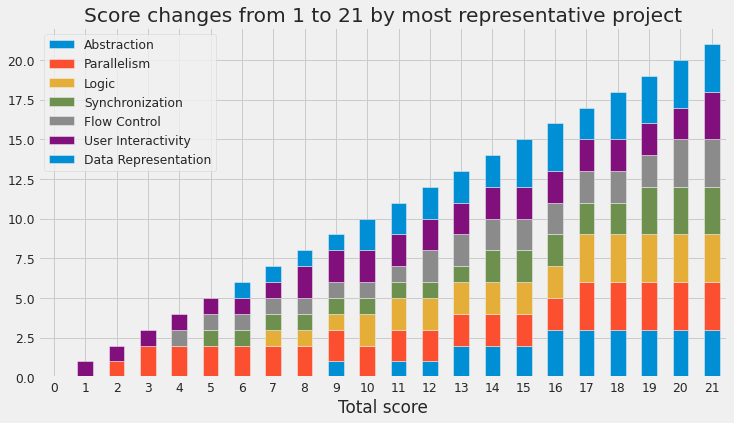
\includegraphics[width=0.8\textwidth]{img/path_CT_Scratch1.png}
    \caption{Ruta de aprendizaje de las dimensiones del PC en Scratch}\label{fig:path_Scratch}
\end{figure}

\begin{itemize}
 \item El cambio de nivel entre 0 y 1: La primera competencia desarrollada es interactividad con el usuario, ya que el programa cuenta con el bloque que inicia su ejecución al pulsar la bandera verde.
 \item El cambio de nivel entre 1 y 2: Como se veía en la distribución~\ref{fig:total2}, los proyectos con 2 puntos cuentan con 2 o más scripts que se ejecutan a la vez al activar la bandera verde.
 \item El cambio de nivel entre 2 y 3: Paralelismo incrementa su valor de 1 a 2 puntos, al incluir las opciones de pulsar una tecla o sobre un objeto como bloques que desencadenan la ejecución simultánea de varios programas o tareas cuando dicho evento se produce.
 \item El cambio de nivel entre 3 y 4: Se implementa cada programa como una sucesión finita y ordenada de pasos concretos y bien definidos, por lo que se empieza a comprender el concepto de algoritmo, y qué fallos acarrea una incorrecta secuenciación. Por ello se asigna un punto a control de flujo. Se define con mayor exactitud lo intuido al comparar las distribuciones~\ref{fig:total3} y~\ref{fig:total4}. 
 \item El cambio de nivel entre 4 y 5: Sincronización empieza a puntuar al usar bloques de espera que establecen el orden temporal en que se ejecutan las tareas de distintos hilos. 
 \item El cambio de nivel entre 5 y 6: Se modifican los atributos asignados a cada personaje u objeto del proyecto, por lo que se logra un punto en representación de los datos.
 \item El cambio de nivel entre 6 y 7: Se comienza a desarrollar el pensamiento lógico, de modo que se implementa una acción determinada sujeta a que se cumpla cierta condición o premisa.
 \item El cambio de nivel o puntuación total entre 7 y 8: Interactividad del usuario pasa a valer 2 puntos, como se indicaba en la distribución~\ref{fig:total8}. Los personajes u objetos son controlados por el teclado o por el ratón. Se gestiona como responde el programa cuando ocurren estos eventos provocados por el usuario.
 \item El cambio de nivel entre 8 y 9: Abstracción es la destreza más compleja y por ello la última en obtener un punto. Se extrae lo relevante de un problema y se descompone en tareas concretas, ejecutadas por varios personajes, más fáciles de implementar, depurar y mantener.
 \item El cambio de nivel entre 9 y 10: En este paso son varias las capacidades que experimentan cambios. Abstracción vuelve a los 0 puntos, mientras que representación de los datos consigue los 2 puntos al utilizar variables como contenedores de un dato que se modifica o que es evaluado para la ejecución de una secuencia de instrucciones. Se emplean por tanto, estructuras selectivas if-else que evalúan una condición determinando por dónde continúa el flujo del programa, y que acción debe llevarse a cabo. Por ello, en lógica se obtienen 2 puntos.
 \item El cambio de nivel entre 10 y 11: Abstracción recupera el punto al implementarse la solución del problema en varios programas más simples y para varios personajes.
 \item El cambio de nivel entre 11 y 12: Se utilizan bucles que repiten la ejecución de sentencias un número determinado o indefinido de veces, reforzando la capacidad de control de flujo que consigue un nivel intermedio de desarrollo valorado con 2 puntos.
 \item El cambio de nivel entre 12 y 13: En abstracción se consiguen 2 puntos. El programador de Scratch define procedimientos o funciones propias que pueden ser reutilizadas en el objeto donde se crearon, llamándolas con los parámetros de entrada que se requieran. 
 \item El cambio de nivel o puntuación total entre 13 y 14: Sincronización toma un valor de 2 puntos. Se emplean el intercambio de mensajes y mecanismos de parada para establecer el orden en que se ejecutan las acciones, de manera que los personajes y programas del proyecto interactúen entre sí.
 \item El cambio de nivel entre 14 y 15: Se declaran listas o estructuras de datos ordenadas, mutables y dinámicas, que almacenan un conjunto de strings o números, requeridos por el programa y cuyos valores son modificados por instrucciones propias de listas durante la ejecución del mismo. Por ello, representación de los datos es la primera capacidad completamente desarrollada y marca el paso al nivel avanzado.
 \item El cambio de nivel entre 15 y 16: Abstracción incrementa su valor a 3 puntos por el uso de clones, que son instancias de un objeto con los mismos atributos y métodos, creados dinámicamente cuando se necesitan varias copias del personaje original con el mismo comportamiento. Facilita el mantenimiento y la modificación del código. 
 \item El cambio de nivel entre 16 y 17: Se utilizan operadores lógicos para evaluar condiciones y decidir si se ejecuta el código implementado asociado. Al combinar el diseño de algoritmos selectivos con la lógica booleana se consigue la máxima puntuación en pensamiento lógico. Paralelismo consigue también 3 puntos, pues se ejecutan simultáneamente varios scripts cuando reciben un mensaje, cambia el escenario o cuando se producen otros eventos multimedia. En representación de los datos se baja a los 2 puntos, pues se emplean variables para almacenar los datos con los que trabaja el programa y no listas.
 \item El cambio de nivel entre 17 y 18: De nuevo se declaran y modifican listas en los programas del proyecto de Scratch. 
 Por lo tanto, representación de los datos vuelve a valer 3 puntos.
 \item El cambio de nivel entre 18 y 19: Se establecen mecanismos de sincronización condicionales o basados en eventos, como el cambio de escenario. La ejecución de un programa continúa cuando se obtiene cierto resultado en otro proceso que envía los datos y espera que sean procesados para continuar con su flujo. Por ello, sincronización vale 3 puntos.
 \item El cambio de nivel entre 19 y 20: Control de flujo alcanza los 3 puntos, puesto que se refuerza la comprensión de los algoritmos iterativos al utilizar bucles sujetos a condiciones. Concuerda con lo obtenido en la distribución ~\ref{fig:total20}. 
 \item El cambio de nivel o puntuación total entre 20 y 21: Se implementan acciones a realizar por los objetos empleando bloques sensores que detectan cambios en la intensidad del sonido o movimiento cuando el usuario emplea el micrófono o la webcam para actuar sobre el proyecto. Interactividad del usuario es la última habilidad que se completa, como ya se indicó en el apartado~\ref{subsec:corr_21_Scratch}. 
\end{itemize}


\section{Análisis de datos de proyectos de Snap!} 
\label{sec:result_snap}

\subsection{Extracción y limpieza de datos}
\label{subsec:clean_data_Snap}

A partir de un directorio de proyectos de Snap! almacenados como ficheros XML, se obtiene la evaluación de los proyectos tras modificar sus métricas y adaptar el código de Dr. Snap!, para que puedan ser analizados a través de su path, gracias a un script de python. Estas evaluaciones son volcadas al fichero \emph{results\_snap\_metrics.csv}. 

En el Jupyter Notebook \emph{ Dr\_Snap\_complete\_analysis.ipynb}\footnote{\url{https://github.com/rcruiz/DrSnap-Analysis}} se cargan los datos del fichero CSV en un dataframe que consta de 113.906 filas y 12 columnas. Por lo tanto, nuestro dataset en bruto está conformado por 113.906 muestras u observaciones que son los proyectos de Snap! caracterizados por 12 atributos o variables. Cada proyecto queda identificado por su nombre y su ruta absoluta. 
Las métricas establecidas para evaluar el desarrollo del pensamiento computacional determinan 7 dimensiones valoradas con puntuaciones enteras entre 0 y 3 puntos, que son: condicionales, sincronización, control de flujo, abstracción, paralelismo, interactividad con el usuario y representación de los datos. Al agregarlas se obtiene otra variable discreta, la puntuación total. A partir de ella se obtiene el valor medio definido en un rango continuo [0, 3] y se asigna un nivel de desarrollo: básico, intermedio y avanzado. Los 5 primeros proyectos y sus atributos correspondientes se reflejan en la figura~\ref{fig:df_Snap}.

\begin{figure}[H]
    \centering
    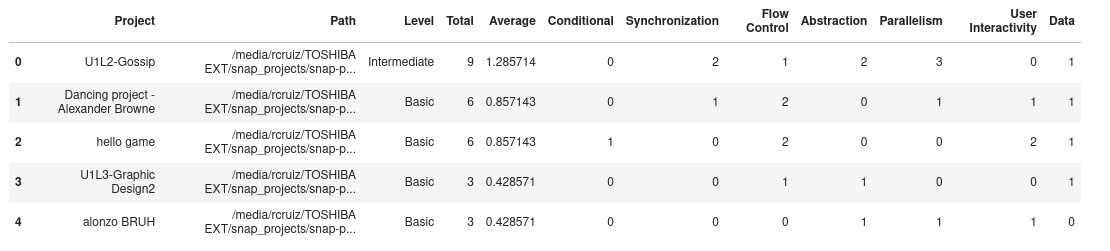
\includegraphics[width=1.0\textwidth]{img/df_origen_Snap.png}
    \caption{Dataframe de los proyectos de Snap! obtenido al cargar \emph{results\_snap\_metrics.csv}}
    \label{fig:df_Snap}
\end{figure}

Se transforman los tipos de datos de la característica nivel a categórico ordinal y de las puntuaciones a enteros sin signo, para facilitar su posterior procesamiento y para que la extensa base de datos ocupe menos en memoria. Se completa la limpieza del conjunto de proyectos eliminando 12 sin nombre asignado y comprobando si existen duplicidades.

Se verifica que existen 56.242 con nombre único aunque todos tienen distinto path. Se debe a que varios programadores de Snap! se basaron en la misma animación o videojuego para implementar e incrementar la complejidad de sus proyectos, siguiendo algún curso, como el propuesto por Berkeley\footnote{\url{https://bjc.edc.org/bjc-r/topic/topic.html?topic=nyc_bjc/1-intro-loops.topic&course=bjc4nyc.html&novideo&noassignment}}. Posteriormente se subieron al repositorio de Snap! con el mismo nombre asignado. De hecho existe un proyecto que es la moda del conjunto total de proyectos, al ser el más frecuente, pues se repite 2.085 veces, ``U1L1-ClickAlonzo'', perteneciente a dicho curso.

\subsection{Análisis de los proyectos de Snap! por nivel o categoría asignada y puntuación total. Distribución de frecuencias}
\label{subsec:frec_nivel_Snap}

¿Cómo es la distribución de los proyectos de Snap! por nivel?

Se continúa explorando la información contenida en los datos clasificando los proyectos de Snap! en función de la categoría de desarrollo alcanzado. Como se visualiza en la figura~\ref{fig:level_Snap}, las frecuencias absolutas y relativas disminuyen según aumenta la complejidad. La mayoría de los proyectos no superan el nivel básico, en concreto un 53,69\% de la población total analizada. El nivel intermedio reúne un 39,17\% del conjunto total, que suponen 44.609 proyectos. Tan solo 8.137 proyectos, un 7,14\%, logran superar el umbral de los 14 puntos. Se debería fomentar el aprendizaje de conceptos y prácticas del pensamiento computacional para que los programadores de Snap! incrementen la dificultad de sus proyectos y se valoren los aspectos más avanzados de cada dimensión. Con ello obtendrían puntuaciones globales mayores y subirían de nivel.

\begin{figure}[H]
    \centering
    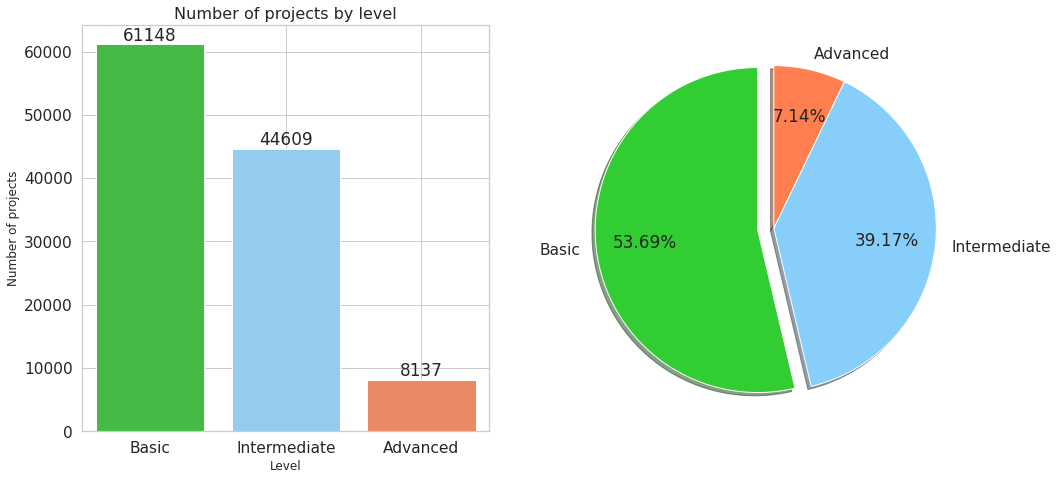
\includegraphics[width=.95\textwidth]{img/freq_level_Snap.png}
    \caption{Distribución de proyectos de Snap! por nivel asignado}\label{fig:level_Snap}
\end{figure}

¿Cómo se distribuyen los proyectos de Snap! entre las puntuaciones asignadas a cada nivel?

Se busca conocer más en detalle cómo se reparten las proyectos según las puntuaciones que determinan la pertenencia a cada una de las tres etapas de desarrollo.

En la distribución~\ref{fig:basic_Snap} del nivel básico, la puntuación nula es la que menos veces aparece. Se incrementa la frecuencia de los proyectos hasta alcanzar un máximo en los 5 puntos, con 14.302 proyectos de Snap! valorados con dicha puntuación. Se mantiene una frecuencia absoluta elevada para las calificaciones de 6 y 7, con 12.134 y 11.529 proyectos respectivamente.

\begin{figure}
    \centering
    \begin{subfigure}[h]{.7\textwidth} 
        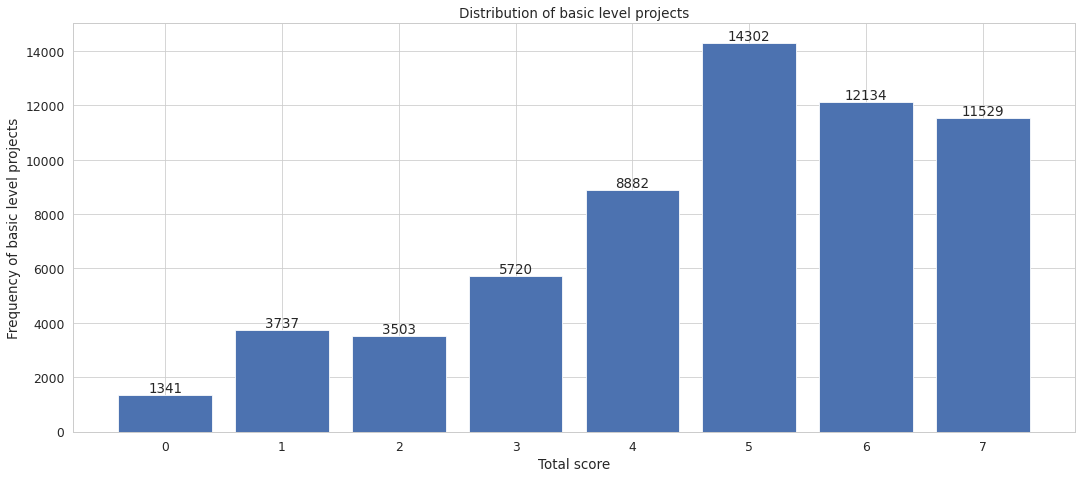
\includegraphics[width=\textwidth]{img/basic_Snap}
        \caption{Nivel básico}
        \label{fig:basic_Snap}
    \end{subfigure}       
    \begin{subfigure}[h]{.7\textwidth} 
        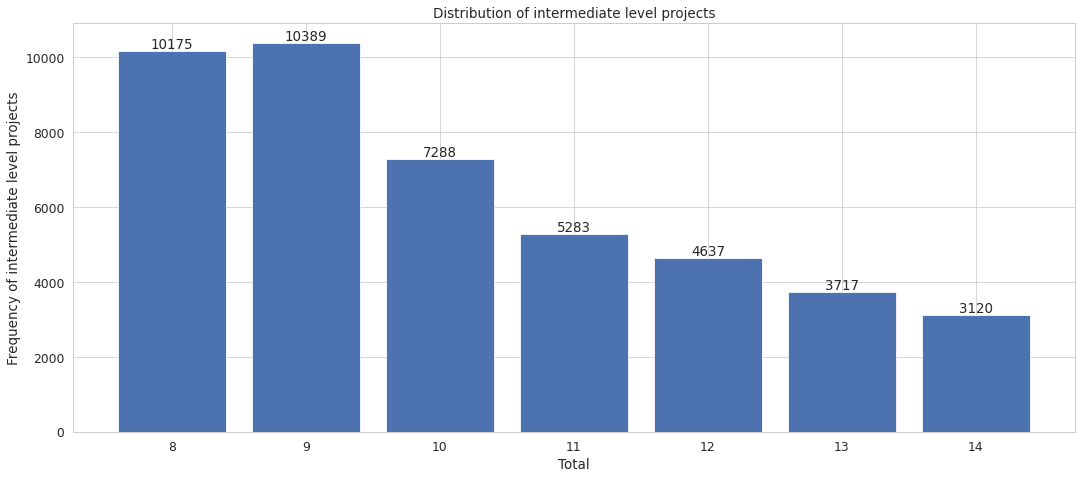
\includegraphics[width=\textwidth]{img/intermediate_Snap}
        \caption{Nivel intermedio}
        \label{fig:intermediate}
    \end{subfigure}
    \begin{subfigure}[h]{.7\textwidth} 
        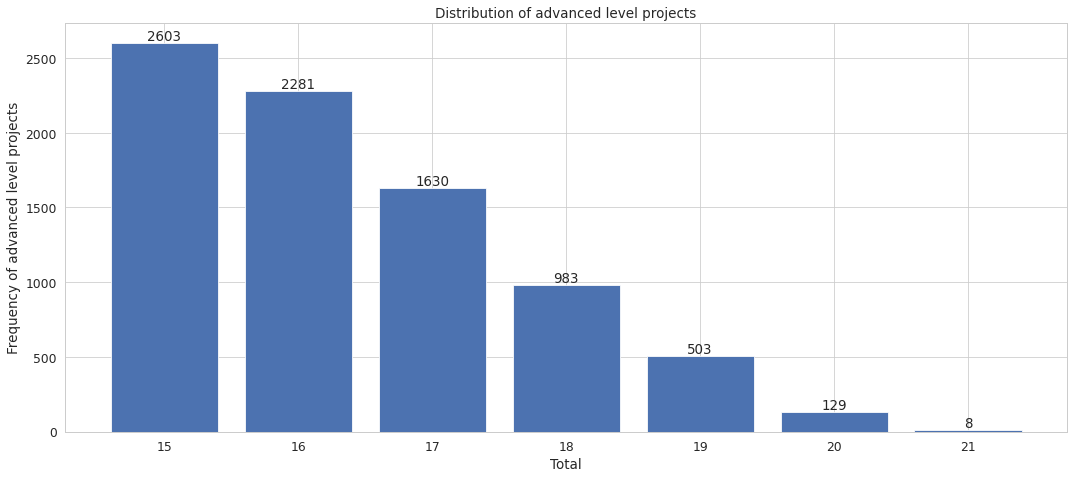
\includegraphics[width=\textwidth]{img/advanced_Snap}
        \caption{Nivel avanzado}
        \label{fig:advanced}
    \end{subfigure}
    \caption{Distribución de proyectos de Snap por puntuaciones asignadas a cada nivel}
\end{figure}

En el nivel intermedio mostrado en la figura~\ref{fig:intermediate}, se sigue una tendencia descendente en las cantidades de proyectos atribuidas a cada puntuación, desde el máximo local situado en los 9 puntos con 10.389 proyectos, hasta los 14 puntos con 3.120 proyectos. Esta tendencia continúa en el nivel avanzado, con 2.603 proyectos valorados con 15 puntos, magnitud que disminuye hasta los ínfimos 129 proyectos que logran 20 puntos y 8 proyectos que consiguen la excelencia en todas las habilidades consideradas, como queda reflejado en la figura~\ref{fig:advanced}.

En la tabla~\ref{table:mean_Snap} se comprueba que al ser la media del nivel básico menor que la mediana, la distribución tiene una asimetría negativa o hacia la izquierda. La mediana coincide con la moda para este nivel. En los niveles intermedio y avanzado la media supera a la mediana, y la asimetría es positiva o hacia la derecha, como también se percibe en los diagramas de barras~\ref{fig:intermediate} y~\ref{fig:advanced}.
Las dispersiones con respecto a la media son más bajas que las obtenidas en Scratch (ver tabla~\ref{table:mean_Scratch}), por lo que la media se ve menos influenciada por puntuaciones extremas. 

\begin{table}[H]
 \begin{center}
  \begin{tabular}{|c|c|c|c|c|}
    \hline
     \textbf{Nivel} & \textbf{Media} & \textbf{Mediana} & \textbf{Varianza} & \textbf{Desviación típica} \\ \hline
    \textbf{Básico} & 4.717211 & 5 & 3.433791 & 1.853049 \\ \hline
    \textbf{Intermedio} & 10.166984 & 10 & 3.520650 & 1.876339 \\ \hline
    \textbf{Avanzado} & 16.375814 & 16 & 1.696996 & 1.302688 \\ \hline
  \end{tabular}
  \caption{Medidas de tendencia central y dispersión para cada nivel de Snap!}
  \label{table:mean_Snap}
 \end{center}
\end{table}

¿Cómo se distribuyen los proyectos de Snap! según la puntuación total?

\begin{figure}[H]
    \centering
    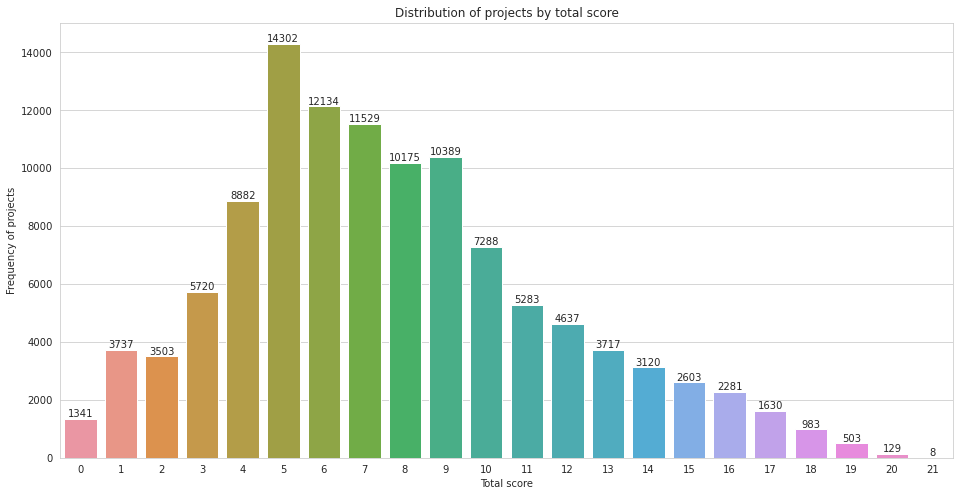
\includegraphics[width=.9\textwidth]{img/frequency_total_score.png}
    \caption{Distribución de proyectos de Snap! por puntuación total.}\label{fig:total}
\end{figure}

Como se aprecia en la figura~\ref{fig:total} existe una mayor concentración de los proyectos entre las puntuaciones totales de 4 y 10 puntos. La moda se localiza en los 5 puntos. La frecuencia decae abruptamente para las puntuaciones más bajas y disminuye de manera más suave para las puntuaciones más altas. Existe una asimetría positiva o hacia la derecha.

Por lo tanto, más de la mitad de los proyectos de Snap! se aglutinan en una etapa inicial o básica de aprendizaje del pensamiento computacional, siendo la calificación total más frecuente 5 puntos. Los programadores de Snap!, cuyos proyectos conforman nuestro dataset, deberían presentar puntuaciones totales superiores si realmente contaran con conocimientos previos. Sería oportuno que recibieran realimentación de cómo mejorar sus proyectos y se sintieran incentivados a incrementar la complejidad de los problemas que resuelven con ellos, para así poder mejorar en las distintas dimensiones y obtener mejores resultados globales. 

\subsection{Frecuencia de los proyectos de Snap! por áreas del pensamiento computacional}
\label{subsec:frec_pc_Snap}

¿Cuál es la distribución de la puntuación en cada dimensión?

Se desglosa en función de cada una de las siete habilidades del PC y se halla la distribución de proyectos para cada puntuación entera entre 0 y 3. Los resultados concretos así como su representación gráfica pueden verse en las figuras~\ref{fig:df_PC_Snap} y~\ref{fig:barras_PC_Snap}. 

\begin{figure}[H]
    \centering      
    \begin{subfigure}[h]{1\textwidth} 
        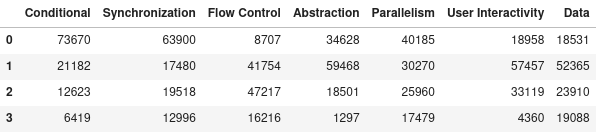
\includegraphics[width=\textwidth]{img/df_PC_Snap.png}
        \caption{Dataframe con la cantidad de proyectos por puntuación y dimensión del PC}
        \label{fig:df_PC_Snap}
    \end{subfigure}
    \begin{subfigure}[h]{1\textwidth} 
        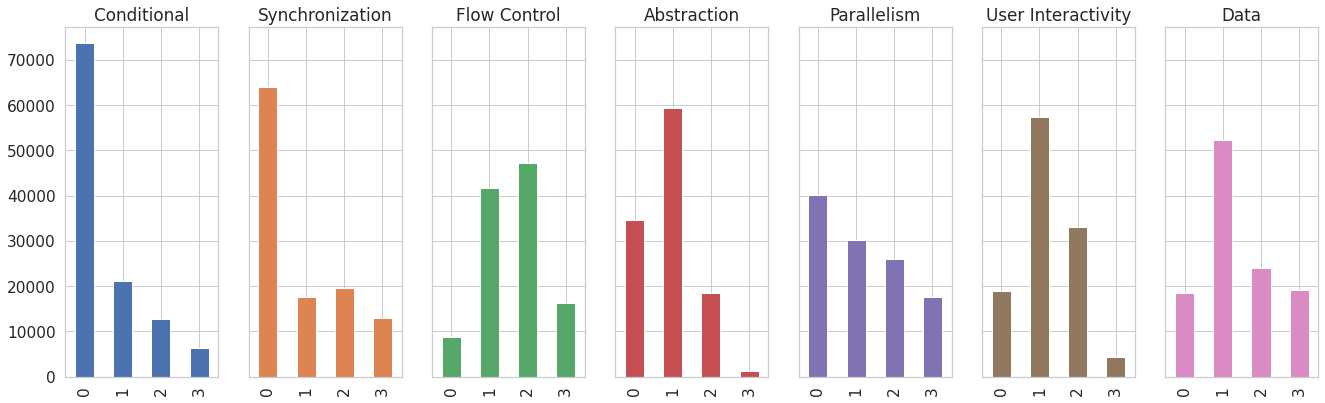
\includegraphics[width=\textwidth]{img/distribution_PC_Snap.png}
        \caption{Diagrama de barras con la cantidad de proyectos por puntuación y dimensión del PC}
        \label{fig:barras_PC_Snap}
    \end{subfigure} 
\caption{Distribución de proyectos de Snap! por puntuación para cada dimensión del PC}
\end{figure}
Se corrobora que las métricas establecidas representen una complejidad creciente que se traduzca en una distribución decreciente, de manera que la cantidad de proyectos que consiguen las puntuaciones más altas en cada capacidad desarrollada sea cada vez menor.   

\begin{itemize}    
    \item \textbf{Condicionales}: Relacionado con el pensamiento lógico que permite discernir qué salidas se generan en función de diferentes situaciones o entradas. Es la habilidad menos desarrollada puesto que 73.670 proyectos no utilizan ni if, ni if-else, ni operadores lógicos como estructuras selectivas que definen por dónde continúa el flujo del programa. Únicamente 21.182 usan un tipo de condicional, y una cantidad aún menor de proyectos emplean 2 o los 3 condicionales especificados, 12.623 y 6.419, respectivamente.    
    \item \textbf{Sincronización}: Es la segunda capacidad menos desarrollada pues en más de la mitad de los proyectos no existen bloques de espera, de parada, de intercambio de mensajes o sujetos a eventos y condiciones que organicen cómo interactúan y se comunican los distintos flujos de código y los personajes del proyecto. % procesos, hilos    
    \item \textbf{Control de flujo}: La mayoría de los proyectos se concentran en torno a 1 y 2 puntos por resolver problemas de manera sistémica, ordenada y precisa mediante algoritmos con un flujo lineal o iterativo con bucles definidos o indefinidos.
    Más de 16.000 proyectos consiguen 3 puntos por utilizar bucles sujetos a condiciones.    
    \item \textbf{Abstracción}: Se aplica un diseño algorítmico basado en la programación modular y en la técnica ``divide y vencerás'' para resolver problemas complejos dividiéndolo en partes más sencillas. Se cuenta con 59.468 proyectos con 1 punto obtenido por contener más de un script y más de un \emph{sprite} o personaje, o una función definida por el programador encargada de una tarea concreta, o clones. Desciende a 18.501 los proyectos que consiguen 2 puntos por usar dos de estas técnicas. Únicamente 1.297 proyectos emplean todos las elementos de abstracción descritos.    
    \item \textbf{Paralelismo}: En 30.270 proyectos se cuenta con un personaje u objeto que realiza simultáneamente varias tareas, mientras que en 25.960 hay 2 o más objetos que ejecutan los mismos programas a la vez, cuando se pulsa una tecla o la bandera verde.
    Disminuye a 17.479 los proyectos con procesos o hilos en paralelo que activan su ejecución cuando reciben mensajes, condiciones o son clones.    
    % Videojuegos en cuenta los eventos que introduce el usuario en el programa
    \item \textbf{Interactividad con el usuario}: La mitad de los proyectos son valorados con 1 punto por implementar acciones que respondan a que el usuario pulse una tecla, la bandera verde o actúe sobre un objeto. Se consiguen 2 puntos en 33.119 proyectos cuando el usuario debe contestar a una pregunta, o mover el ratón o un personaje. Solo en 4.360 proyectos los objetos son controlados por las modificaciones de audio o vídeo que introduce el usuario durante su ejecución.    
    \item \textbf{Representación de los datos}: La capacidad que indica cómo se manejan y abstraen los datos requeridos por los programas consigue puntuaciones en sentido descendente. Hay más de 50.000 proyectos donde se especifican los atributos de los personajes, 23.910 en los que se declaran y modifican variables y 19.088 que cuentan con operaciones sobre listas. 
\end{itemize}    

\subsection{Análisis estadístico general de las dimensiones del pensamiento \\computacional con Snap!}
\label{subsec:estad_pc_Snap}

Se sigue con el análisis exploratorio de los datos desde un enfoque descriptivo univariante calculando las medidas de tendencia central, variabilidad y posición que resumen y caracterizan cada variable analizada del pensamiento computacional. Se reflejan en la figura~\ref{fig:describe_Snap}.

\begin{figure}[H]
    \centering
    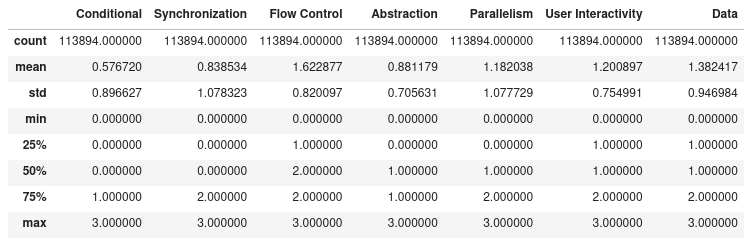
\includegraphics[width=1\textwidth]{img/describe_Snap.png}
    \caption{Media, desviación estándar y cuartiles de cada CT}
    \label{fig:describe_Snap}
\end{figure}

Control de flujo y representación de los datos consiguen las mayores medias y medianas, por lo que se deduce que son las destrezas que se adquieren con más facilidad, mientras que las menores medias y medianas son para condicionales y sincronización. El hecho de que no se apliquen en la mitad de los proyectos puede deberse a que no se requiera o resulten complicadas. Las habilidades con menor dispersión con respecto a la media son abstracción, interactividad con el usuario y control de flujo, como se concluye a partir de la desviación típica. Para el resto de capacidades su valor es elevado, en torno a 1,
por lo que la mediana será más representativa que la media. En la figura~\ref{fig:describe_Snap} se indica además el valor de los cuartiles, que serán estudiados con mayor detalle en el diagrama de cajas~\ref{fig:cajas_Snap}.
Nos muestra la dispersión de los proyectos ordenados de menor a mayor puntuación y podemos identificar si existen valores atípicos. Al representarlos en el mismo gráfico se puede comenzar a intuir alguna relación entre las dimensiones, aunque se siga con el análisis univariante.

\begin{figure}[H]
    \centering
    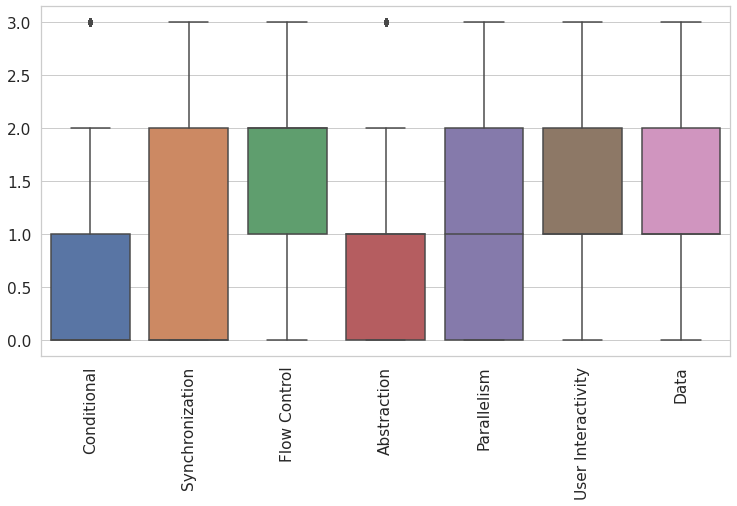
\includegraphics[width=0.7\textwidth]{img/diag_cajas_Snap.png}
    \caption{Diagrama de cajas de cada dimensión del CT}
    \label{fig:cajas_Snap}
\end{figure}

\begin{itemize}
    \item \textbf{Condicionales, sincronización y abstracción}: Como ya se ha indicado la mitad de los proyectos no consiguen puntuar en condicionales y sincronización, estando el primer y el segundo cuartil en 0 puntos. Sin embargo, en sincronización el rango intercuartílico es de 2 puntos, implicando mayor dispersión de proyectos de Snap! entre la mediana y el $Q_3$ y que los 3 puntos marquen el límite superior, en vez de ser considerados valores atípicos o \emph{outliers}. Los proyectos con 3 puntos también son \emph{outliers} en abstracción, aunque igualmente válidos en nuestro estudio. En dicha dimensión, el 25\% de los proyectos tienen 0 puntos, la mitad de los proyectos son evaluados con 0 o 1 punto, y todos los proyectos entre la mediana y el tercer cuartil, se concentran en 1 punto. % Como 1.5 * Rango intercuartil + Q3 = 2.5 
    \item \textbf{Paralelismo}: Su rango intercuartil es de 2 puntos con la mediana en 1 punto. Con respecto a las otras habilidades, las puntuaciones de los proyectos presentan mayor dispersión a ambos lados de este valor central, de modo que la mitad de los proyectos tienen 0 y 1 puntos, al llegar al $Q_3$ algunos obtienen 2 puntos, y el límite superior está en 3 puntos.
    \item \textbf{Interactividad con el usuario, representación de los datos y control de flujo}: Las tres capacidades concentran la mitad de los proyectos entre 1 y 2 puntos, como se aprecia en el rango intercuartílico comprendido entre $Q_1$ y $Q_3$. Los proyectos están más dispersos para las puntuaciones inferiores en control de flujo, como se deduce de la posición del $Q_1$ y del $Q_2$, que para las puntuaciones superiores. Los valores se concentran en torno a 2 puntos, donde mediana y $Q_3$ coinciden. En cambio, en las otras dos capacidades, la asimetría es hacia la derecha, pues la primera mitad de los proyectos logran 1 punto, mientras que en la mitad superior obtienen valores entre 1, 2 y 3 puntos.
\end{itemize}

Para profundizar en las relaciones que puedan establecerse entre las habilidades y entre éstas con el total, se recurre al análisis descriptivo bivariante y en concreto a los coeficientes de correlación lineal de Pearson. Primero, se comprueba si existe una asociación lineal perfecta entre cada una de las capacidades consideradas del pensamiento computacional con la puntuación total obtenida. Se recogen en la tabla~\ref{table:corr_total_Snap} los valores de los coeficientes. 
El menor grado de dependencia lineal con el total se produce en representación de los datos y abstracción. Al desarrollarse estas dimensiones, la puntuación total aumenta en menor medida que si se fomentan el resto de habilidades. Serían las que más información y expresividad aportan. Tanto en paralelismo como en sincronización existe una elevada dependencia lineal con el total.

\begin{table}[htbp]
 \begin{center}
 \resizebox{15cm}{!} {
    \begin{tabular}{|c|c|c|c|c|c|c|c|}
    \hline
    \textbf{Correlación} & \textbf{Condicionales} & \textbf{Sincronización} & \textbf{Control de flujo} & \textbf{Abstracción} & \textbf{Paralelismo} & \textbf{\begin{tabular}[c]{@{}c@{}}Interactividad\\ con el usuario\end{tabular}} & \textbf{\begin{tabular}[c]{@{}c@{}}Representación\\ de los datos\end{tabular}} \\
    \hline
    \textbf{Total} & 0.641439 & 0.734082 & 0.595380 & 0.514194 & 0.740135 & 0.667972 & 0.491424 \\
    \hline
    \end{tabular} }
    \caption{Correlación de la puntuación total con cada dimensión del PC}
    \label{table:corr_total_Snap}
 \end{center}
\end{table}

Es precisamente entre sincronización y paralelismo donde existe mayor dependencia lineal en sentido positivo, como se observa en la matriz de correlación~\ref{fig:corr_Snap}.
Cuando en un proyecto de Snap! se ejecutan varios flujos de código a la vez, se necesitan mecanismos que organicen esa ejecución simultánea. Condicionales e interactividad con el usuario presentan una correlación positiva moderada. Cuando el usuario interactúa con el proyecto moviendo los objetos, con el ratón o pulsando una tecla y contestando a preguntas,
se incrementa el uso de condicionales, seleccionando el conjunto de sentencias a ejecutar según la acción realizada. Abstracción y control de flujo son independientes linealmente. La descomposición del problema en scripts y funciones propias encargadas de tareas concretas no guarda relación con las nociones algorítmicas demostradas en cada script o función.
Interactividad con el usuario y abstracción y representación de los datos con el resto de dimensiones también están incorreladas, con valores de $\rho\approx0$.

\begin{figure}[H]
    \centering
    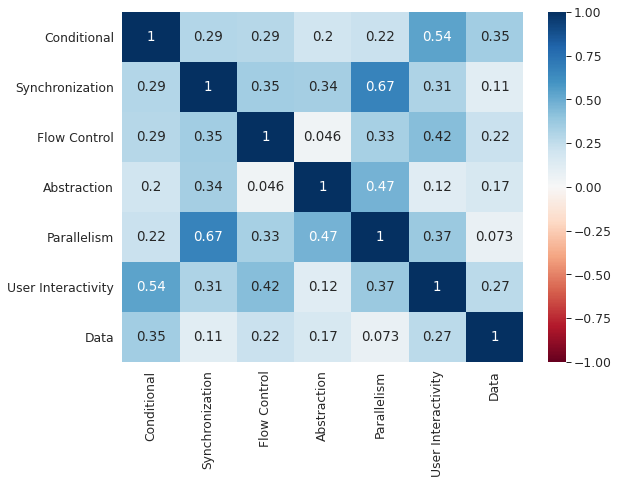
\includegraphics[width=.7\textwidth]{img/corr_Snap.png}
    \caption{Matriz de correlación de Pearson de las dimensiones del PC.}\label{fig:corr_Snap}
\end{figure}

\subsection{Frecuencias y correlaciones de las dimensiones del PC en función de la puntuación total para proyectos de Snap!}
\label{subsec:corr_21_Snap}

Se busca ver la evolución de las correlaciones existentes entre cada par de habilidades según se incrementa la complejidad global de los proyectos, así como la distribución de puntuaciones en cada habilidad para cada puntuación total. Podemos hacernos una idea de qué habilidades son más difíciles de adquirir y de cómo los programadores de Snap! progresan en ellas.

Como en el apartado~\ref{subsec:corr_21_Scratch}, se descartan los valores mínimo y máximo de la puntuación total, ya que todas las habilidades tienen la misma puntuación en cada proyecto de Snap! y no existen variaciones con respecto al valor medio, ni entre cada par de variables de manera conjunta, ni en cada una de ellas por separado. Así la covarianza y la desviación típica son nulas cuando el total es 0 o 21 y el cálculo de su coeficiente de correlación no tiene sentido (ver fórmula~\eqref{eq:correlacion}). 

%%Resumen
Se recogen en el apéndice~\ref{append_Snap} las valoraciones y las correlaciones entre las dimensiones según se avanza gradualmente a mayores niveles de destreza global. Se indican a continuación las dependencias que persisten en rangos de puntuación total más amplios.

Representación de los datos conserva correlaciones casi perfectas con interactividad con el usuario desde los 3 hasta los 18 puntos totales. Cuando se gestionan las acciones que realiza el usuario sobre el programa, se modifican los datos de los atributos de los objetos, de las variables y de las listas. Ambas presentan interdependencias muy elevadas con control de flujo entre los 8 y los 14 puntos, aumentando las nociones algorítmicas cuando se emplean.

Es precisamente a partir de los 14 puntos globales cuando control de flujo se relaciona de manera perfecta en sentido positivo con sincronización. Al utilizar bucles definidos, infinitos o condicionales, aumenta el intercambio de mensajes y la interrupción en la ejecución de un script hasta que se produzca cierto estado o evento en otro proceso. Ambas mantienen fuertes correlaciones con paralelismo, desde los 9 puntos con control de flujo y desde los 12 puntos con sincronización. La ejecución simultánea de varios scripts depende de los mecanismos de sincronización citados para que se produzca y a su vez, estas secuencias de instrucciones van incluyendo estructuras iterativas según los proyectos tienden a niveles de competencia mayores.

%Según aumenta el uso de estructuras iterativas condicionales y se utilizan mecanismos más avanzados que establecen el orden en que se ejecutan los procesos,  
%%


\subsection{Aprendizaje no supervisado: clustering K-Means en proyectos de Snap!}
\label{subsec:kmeans_Snap}

Tras el análisis de las correlaciones entre cada par de habilidades para cada grupo de proyectos según su nivel de complejidad total, se construye un modelo de aprendizaje no supervisado que agrupe proyectos similares en base a la semejanza inherente de sus características o dimensiones. El clustering K-Means segmenta los 113.894 proyectos de Snap! en k grupos disjuntos, asignando cada proyecto definido como un vector de siete dimensiones al centro del clúster más cercano. Mediante un proceso iterativo el algoritmo busca minimizar las distancias intra-clúster y por lo tanto la inercia, provocando que se incrementen las distancias inter-clúster. 

Las métricas utilizadas para estimar el número de grupos en que dividir nuestra población de proyectos, calculan y relacionan estas distancias de distintas maneras, tal como veíamos en la sección~\ref{sec:k_means diseño}. La elección de un número de grupos óptimo es un requisito indispensable para que el algoritmo se ejecute y nos permita distinguir pautas relevantes y extraer conclusiones certeras a través de los proyectos representativos de cada grupo. Para ello, iteramos sobre una secuencia de valores de k y obtenemos la representación gráfica de las métricas en la figura~\ref{fig:determine_k}.

En la curva de Elbow de la figura~\ref{fig:determine_k}, la inercia o suma de los cuadrados de la distancia intra-clúster disminuye sin experimentar cambios abruptos en su pendiente según aumenta el número de grupos. El valor óptimo de k estará en el rango [8, 15]. En dicho rango los proyectos de Snap! de cada clúster mantienen su similitud por su cercanía al centroide del grupo sin que una elevada segmentación provoque que proyectos similares pertenezcan a grupos diferentes. 

\begin{figure}[H]
    \centering
    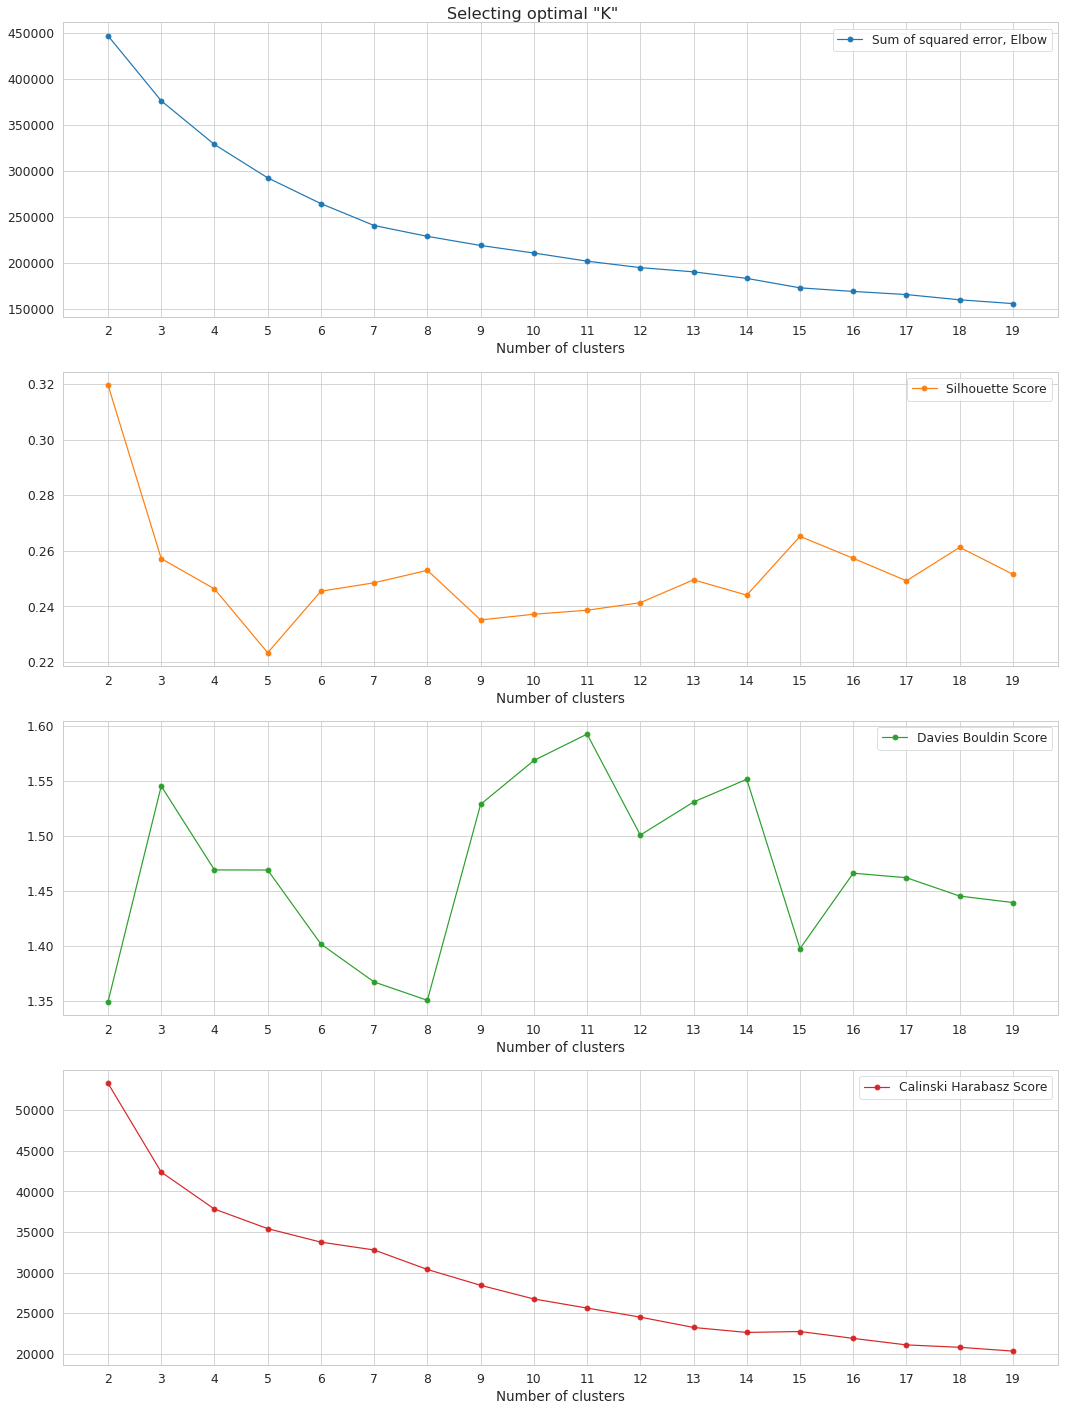
\includegraphics[height=.58\textheight]{img/select_k.png}
    \caption{Métodos para determinar el valor de k}\label{fig:determine_k}
\end{figure}

Para acotar el rango de k se recurre al análisis de la silueta. Sus coeficientes toman valores en el intervalo [-1, 1]. Como se indicaba en la ecuación~\eqref{eq:silueta}, valores próximos a 1 establecen grupos densos y suficientemente distantes o separados de los clústeres vecinos para que ningún proyecto esté incorrectamente asignado. En su representación en la figura~\ref{fig:determine_k} encontramos un máximo global en k=15, y dos máximos locales en k=8 y en k=18. Se descarta este último valor, ya que conlleva una elevada segmentación. Sin embargo los valores de los coeficientes están muy juntos, entre 0,2233 y 0,265 para cada k analizado. Se recurre a otros dos índices de validación interna del clustering. 

Según los criterios establecidos en el diagrama~\ref{fig:kmeans}, el índice de Davies-Bouldin busca valores próximos a 0, que minimicen la dispersión intra-clúster de los dos grupos más similares y maximice la distancia entre sus centroides. En nuestro caso, existe un mínimo global en k=8 y otro mínimo local en k=15, coincidiendo con los valores que cumplen los requisitos del método de la silueta. El índice de Calinski-Harabasz no aporta demasiada información, puesto que no hay ningún valor de k donde el ratio entre las varianzas inter-partición e intra-partición se haga máximo.

\subsubsection{Similitudes y diferencias entre clustering k-means con k=8 y k=15}
\label{sec:k8_k15}

Para discernir si es mejor dividir nuestros proyectos en 8 grupos o en 15 grupos se realiza un estudio exhaustivo de las similitudes y diferencias que presentan las agrupaciones, tanto por los proyectos que contienen como por las habilidades que caracterizan a cada grupo.

El algoritmo K-Means parte de 8 centroides localizados en posiciones aleatorias. Se asignan los proyectos al centroide más cercano, se calcula la media de los proyectos de cada clúster y se colocan los centroides en dichas medias. Se repite la reasignación de centros y proyectos hasta alcanzar la convergencia. Se consigue así minimizar la distancia cuadrática media intra-clúster o varianza interna de cada clúster, de forma que los centroides o medias representan a cada grupo. Se buscan los proyectos de Snap! más cercanos a los 8 centros, que son los que definen al grupo según las 7 características discretas del pensamiento computacional.

\begin{table}
    \centering
    \resizebox{10cm}{!}{
    \begin{tabular}{lrrrrrrrr}
        \cline{2-9}
        {} & \multicolumn{8}{c}{\cellcolor[HTML]{FFCCC9}\textbf{Clúster}} \\ \hline
        {} & \textbf{0} & \textbf{1} & \textbf{2} & \textbf{3} & \textbf{4} & \textbf{5} & \textbf{6} & \textbf{7} \\ \hline
        \textbf{Condicionales} & 0 & 2 & 0 & 0 & 2 & 0 & 0 & 1 \\
        \textbf{Sincronización} & 0 & 3 & 0 & 0 & 0 & 2 & 0 & 2 \\
        \textbf{Control de flujo} & 2 & 2 & 0 & 2 & 2 & 2 & 1 & 2 \\
        \textbf{Abstracción} & 0 & 2 & 1 & 1 & 1 & 1 & 1 & 0 \\
        \textbf{Paralelismo} & 1 & 3 & 0 & 2 & 1 & 3 & 0 & 1 \\
        \textbf{Interactividad con usuario} & 1 & 2 & 0 & 1 & 2 & 1 & 1 & 2 \\
        \textbf{Representación de datos} & 1 & 2 & 0 & 1 & 2 & 1 & 3 & 2 \\ \hline
        \textbf{Total} & 5 & 16 & 1 & 7 & 10 & 10 & 6 & 10 \\ \hline
    \end{tabular}}
    \caption{Puntuaciones de los proyectos representativos para el clustering con k=8}
    \label{table:representative_k8}
\end{table}

Según la tabla~\ref{table:representative_k8}, los clústeres 0, 2, 3 y 6 pertenecen al nivel básico. En todos ellos, condicionales y sincronización no puntúan y paralelismo es la capacidad que más difiere. La puntuación total más baja es la del prototipo del grupo 2, con un único punto en abstracción. Los proyectos más representativos del nivel intermedio están evaluados con 10 puntos totales, y son los clústeres 4, 5 y 7. El clúster 4 y el 7 presentan el mismo nivel de desarrollo en interactividad con el usuario, representación de los datos, paralelismo y control de flujo. El clúster 5 coincide con el clúster 4 en abstracción y con el clúster 7 en sincronización. En las tres agrupaciones de nivel intermedio control de flujo vale 2 puntos. El clúster 1 representa al nivel avanzado con 16 puntos totales. Solo alcanza los valores máximos en sincronización y paralelismo, mostrando una comprensión plena de la concurrencia entre los procesos que provoca la interacción de los personajes, permitiendo la ejecución simultánea de tareas independientes.

Se vuelve a aplicar el algoritmo K-Means, siendo en esta ocasión 15 el número de grupos en que se segmenta el conjunto de proyectos o datos de entrada. La inercia obtenida es menor cuando se estabiliza la posición de los centroides y no hay reasignación de proyectos a dichos centros. Los proyectos dentro de cada grupo serán más similares entre sí, al estar más concentrados en torno al centro. Se coteja si los 15 grupos difieren entre sí a partir de los proyectos que los identifican, reflejados en la tabla~\ref{table:representative_k15}.

\begin{table}[H]
    \centering
    \resizebox{15cm}{!}{
    \begin{tabular}{lrrrrrrrrrrrrrrr}
        \cline{2-16}
        {} & \multicolumn{15}{c}{\cellcolor[HTML]{CBCEFB}\textbf{Clúster}} \\ \hline
        {} & \textbf{0} & \textbf{1} & \textbf{2} & \textbf{3} & \textbf{4} & \textbf{5} & \textbf{6} & \textbf{7} & \textbf{8} & \textbf{9} & \textbf{10} & \textbf{11} & \textbf{12} & \textbf{13} & \textbf{14} \\ \hline
        \textbf{Condicionales} & 1 & 0 & 0 & 2 & 0 & 0 & 1 & 0 & 0 & 1 & 1 & 2 & 2 & 0 & 1 \\
        \textbf{Sincronización} & 2 & 0 & 2 & 0 & 0 & 0 & 3 & 0 & 0 & 2 & 0 & 0 & 3 & 0 & 0 \\
        \textbf{Control de flujo} & 2 & 2 & 1 & 1 & 2 & 0 & 2 & 2 & 1 & 2 & 3 & 2 & 3 & 1 & 1 \\
        \textbf{Abstracción} & 2 & 0 & 1 & 1 & 1 & 1 & 1 & 1 & 1 & 0 & 0 & 1 & 2 & 1 & 0 \\
        \textbf{Paralelismo} & 3 & 1 & 3 & 1 & 2 & 0 & 3 & 0 & 0 & 1 & 0 & 2 & 2 & 1 & 0 \\
        \textbf{Interactividad con usuario} & 1 & 1 & 1 & 2 & 1 & 0 & 2 & 0 & 0 & 1 & 2 & 2 & 2 & 2 & 2 \\
        \textbf{Representación de datos} & 2 & 1 & 1 & 2 & 1 & 0 & 1 & 1 & 3 & 2 & 2 & 1 & 2 & 3 & 0 \\ \hline
        \textbf{Total} & 13 & 5 & 9 & 9 & 7 & 1 & 13 & 4 & 5 & 9 & 8 & 10 & 16 & 8 & 4 \\ \hline
    \end{tabular}}
    \caption{Puntuaciones de los proyectos representativos para el clustering con k=15}
    \label{table:representative_k15}
\end{table}

En el nivel básico están los clústeres 1, 4, 5, 7, 8, 14. Todos menos el clúster 14 tienen 0 puntos en condicionales y sincronización. El clúster 5 es el que presenta menor puntuación con 1 punto total en abstracción. 
En el nivel intermedio se encuentran los clústeres 0, 2, 3, 6, 9, 10, 13. El clúster 3 y el clúster 13 son muy similares, pues solo difieren en condicionales y en datos. Lo mismo ocurre entre el clúster 0 y el 9, que se diferencian en la valoración de abstracción y paralelismo. Hay tres agrupaciones cuyos proyectos más representativos tienen 9 puntos totales, que son los clústeres 2, 3 y 9. El clúster 0 y el clúster 6 coinciden en puntuación total. En el nivel avanzado solamente está el clúster 12 con 16 puntos totales, que cuenta con 3 puntos en sincronización y en control de flujo y 2 puntos en el resto de capacidades.

%Al no disponer a priori de una respuesta etiquetada con la que comparar las etiquetas obtenidas tras el agrupamiento
Se analiza a continuación cómo se disgregan los grupos del clustering con k=8 cuando se transforman en los 15 grupos del clustering con k=15, a partir de los proyectos que tienen en común. Se impone que la coincidencia supere el 5\%. Como se recoge en la tabla~\ref{table:comparativa_k}, prácticamente cada clúster de k=8 posee una similitud cercana o superior al 60\% con un único clúster de k=15. De hecho, los proyectos representativos de los clústeres 0, 2 y 3 con k=8 coinciden con los que definen los grupos 1, 5 y 4 de k=15, respectivamente, en las valoraciones recibidas en cada dimensión del pensamiento computacional. 

Sin embargo, el clúster 4 se disgrega en 5 grupos para k=15, con un 40\% de parecido con el clúster 3 y una similitud inferior con el 10, el 11, el 13 y el 14. Calculando la media de la intersección de cada uno con el grupo 4 de k=8, se ven las diferencias entre las dimensiones analizadas que provocan su división en diferentes grupos. Los proyectos del clúster 3 se distinguen por emplear entre 2 y 3 tipos de condicionales. Los pertenecientes al clúster 10 se diferencian por utilizar bucles que iteran hasta que se cumple cierta condición, por lo que la puntuación media en control de flujo es la más elevada. El clúster 11 tiene la mayor media en paralelismo. El clúster 14 posee la valoración media más baja en representación de los datos. El clúster 13 difiere de los demás en todas las dimensiones expuestas.

Por lo tanto, dada la similitud existente entre cada grupo del clustering con k=8 con un único grupo del clustering con k=15,  parece recomendable quedarse con la segmentación en 8 grupos. Aunque establecer un itinerario de aprendizaje a partir de sus proyectos representativos no resulta tan evidente como con Scratch.

\subsection{Análisis de clustering entre niveles o puntuaciones totales. Ruta de aprendizaje demostrada en los proyectos de Snap!}
\label{subsec:ruta_Snap}

De una forma equivalente a la planteada con Scratch en el apartado~\ref{subsec:ruta_Scratch}, se agrupan los proyectos por puntuación total y se obtiene el proyecto prototipo de cada grupo, para definir el proceso de aprendizaje gradual en función de sus dimensiones. 

\begin{figure}[H]
    \centering
    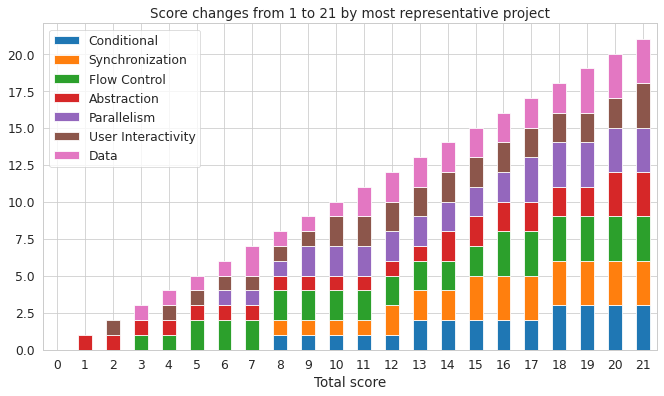
\includegraphics[width=.8\textwidth]{img/path_CT_Snap.png}
    \caption{Ruta de aprendizaje de las dimensiones del PC en Snap!}\label{fig:path_Snap}
\end{figure}

Así según la figura~\ref{fig:path_Snap} se perfila de una manera más clara que en las distribuciones del apéndice~\ref{append_Snap} la habilidad cuyo desarrollo provoca el paso al siguiente nivel de complejidad. 

\begin{itemize}
 \item El cambio de nivel entre 0 y 1:  La primera dimensión en puntuar es abstracción. Se descompone el problema en partes más sencillas, para cuya resolución se emplean varios scripts y personajes o funciones implementadas por el programador encapsuladas dentro de un bloque personalizado o instancias del objeto. Resulta bastante llamativo. Podría deberse a la relevancia dada en los cursos de Snap! a la creación de funciones propias.
 \item El cambio de nivel entre 1 y 2: Se consigue 1 punto en interactividad con el usuario. Los scripts comienzan a ejecutarse cuando se produce un evento o detectan una acción del usuario, como pulsar una tecla, la bandera verde o un objeto.
 \item El cambio de nivel entre 2 y 3: Interactividad con el usuario ya no puntúa. Se obtiene 1 punto en control de flujo y en representación de los datos. Los proyectos están programados siguiendo una secuencia de instrucciones concreta, precisa y finita que demuestra ciertas nociones algorítmicas y se modifican las propiedades o atributos de los objetos.
 \item El cambio de nivel entre 3 y 4: Interactividad con el usuario vuelve a conseguir 1 punto.
 \item El cambio de nivel entre 4 y 5 puntos: Control de flujo alcanza un nivel intermedio. Se incluyen bucles en el programa, de modo que se repite la ejecución de sentencias un número determinado de veces o de manera indefinida. %%
 \item El cambio de nivel entre 5 y 6 puntos: Paralelismo comienza a puntuar. Se programa para que el objeto realice varias acciones simultáneamente al pulsar teclas o la bandera verde.
 \item El cambio de nivel entre 6 y 7 puntos: Representación de los datos vale 2 puntos. Se declaran y modifican variables cuyos datos permiten la correcta ejecución de los programas.
 \item El cambio de nivel entre 7 y 8 puntos: Datos decrementa su valor a 1 punto, de forma que únicamente se realizan operaciones sobre los atributos de los objetos y no sobre variables. Condicionales y sincronización puntúan. Se utiliza un tipo de estructura condicional para decidir por donde continua el flujo del programa ante la evaluación de alguna situación. Además, mientras un programa ejecuta instrucciones el otro espera a que termine para ejecutar las que le corresponden, siguiendo un orden temporal preestablecido.
 \item El cambio de nivel entre 8 y 9 puntos: Paralelismo consigue 2 puntos. Varios personajes u objetos ejecutan el mismo o varios programas simultáneamente al pulsar una tecla o la bandera verde, de manera que se resuelven tareas concretas a la vez.
 \item El cambio de nivel entre 9 y 10 puntos: Interactividad con el usuario incrementa su calificación a 2 puntos. Se requiere en el programa que el usuario responda a preguntas, mueva el ratón o se pulse sobre determinado objeto, para que se desencadene la ejecución de sentencias sujetas a dichos eventos.
 \item El cambio de nivel entre 10 y 11 puntos: En datos se vuelve a los 2 puntos. De nuevo se declaran y modifican variables que almacenan los datos requeridos por el programa.
 \item El cambio de nivel entre 11 y 12 puntos: Sincronización vale 2 puntos. Los programas intercambian entre sí mensajes o paran su ejecución según lo que ocurra en otros scripts.
 \item El cambio de nivel entre 12 y 13 puntos: Condicionales aumenta su puntuación a 2 puntos. Se utilizan dos tipos de sentencias condicionales, que seleccionan el conjunto de instrucciones que se ejecutará en función de la evaluación de una situación o de varias si se emplean operadores lógicos. Se desarrolla el pensamiento lógico.
 \item El cambio de nivel entre 13 y 14 puntos: En abstracción se obtienen 2 puntos. Se emplean dos de las técnicas consideradas, varios objetos y scripts, clones o bloques definidos por el programador, que en conjunto son capaces de resolver un problema más complicado.
 \item El cambio de nivel entre 14 y 15 puntos: Sincronización se desarrolla por completo. Los programas del proyecto interactúan entre sí siguiendo un orden preestablecido basado en eventos, condiciones o  mensajes a un objeto concreto. 
 \item El cambio de nivel entre 15 y 16 puntos: Control de flujo alcanza su máxima valoración al utilizarse bucles condicionales.
 \item El cambio de nivel entre 16 y 17 puntos: Paralelismo obtiene 3 puntos. Uno o varios objetos ejecutan scripts a la vez cuando se cumple cierta condición, reciben un mensaje o son instancias de objetos que deben realizar las mismas tareas o instrucciones.
 \item El cambio de nivel entre 17 y 18 puntos: Condicionales incrementa su valor a 3 puntos. Se emplean los tres tipos de sentencias condicionales: if, if-else y operadores lógicos que evalúan que se cumplan ciertas situaciones para decidir qué conjunto de bloques ejecutar. Se consiguen proyectos dinámicos que obtienen salidas diferentes en función de la evaluación de premisas o situaciones.
 \item El cambio de nivel entre 18 y 19 puntos: Representación de los datos consigue 3 puntos. Se definen listas y se realizan operaciones sobre ellas y sobre los elementos que contienen. Se pueden formar estructuras de datos más complejas, como listas de listas, listas con resultados de funciones o cualquier conjunto de elementos de primera clase.
 \item El cambio de nivel entre 19 y 20 puntos: Abstracción aumenta su puntuación a los 3 puntos. Se descompone la resolución del problema en tareas más sencillas en las que se extrae lo más relevante para encontrar patrones y poder resolver tareas similares con los mismos scripts o funciones propias definidas por el programador. Por lo tanto se emplean varios scripts y objetos, clones y bloques creados de cualquier tipo.
 \item El cambio de nivel entre 20 y 21 puntos: Interactividad con el usuario es la última en desarrollarse por completo. En los programas se detectan colisiones entre objetos y se gestiona audio o vídeo que el usuario introduce durante la ejecución del programa.
\end{itemize} 
 

%%%%%%%%%%%%%%%%%%%%%%%%%%%%%%%%%%%%%%%%%%%%%%%%%%%%%%%%%%%%%%%%%%%%%%%%%%%%%%%%
%%%%%%%%%%%%%%%%%%%%%%%%%%%%%%%%%%%%%%%%%%%%%%%%%%%%%%%%%%%%%%%%%%%%%%%%%%%%%%%%
% CONCLUSIONES %
%%%%%%%%%%%%%%%%%%%%%%%%%%%%%%%%%%%%%%%%%%%%%%%%%%%%%%%%%%%%%%%%%%%%%%%%%%%%%%%%

\cleardoublepage
\chapter{Conclusiones}
\label{chap:conclusiones}

\section{Consecución de objetivos}
\label{sec:consecucion-objetivos}

Los objetivos propuestos en el capítulo~\ref{chap:objetivos} han sido alcanzados, en términos generales. La importancia de este estudio radica en el volumen de datos analizados, por ello no se tomaron muestras y se decidió realizar el estudio con ambos grupos analizados en su completitud.

En primer lugar había que extraer y recolectar en un fichero csv todas las métricas relevantes para conocer el impacto de cada herramienta en el desarrollo del pensamiento computacional. Se corrigieron los errores de formato y se buscó que las variables analizadas fueran comparables,  discriminantes y expresivas para ambas poblaciones, descartando una ínfima cantidad de proyectos del estudio.

Para dar cumplimiento al segundo objetivo hay que matizar que son análisis cuantitativos estáticos, puesto que no se conocen las cualidades de las poblaciones, solo los valores asignados a las dimensiones en cada una de sus creaciones o artefactos. No obstante, se puede extrapolar de lo indicado sobre Scratch (sección~\ref{sec:scratch}) y Snap! (sección~\ref{sec:snap}), que los \emph{scratchers} suelen ser escolares sin conocimientos computacionales previos, mientras que el público objetivo de Snap! son jóvenes que quieren potenciar sus habilidades computacionales a través de la programación.

Sin embargo, la proporción de proyectos de Snap! de nivel avanzado es 5 puntos porcentuales inferior, que se transfieren a un nivel básico, al comparar los diagramas~\ref{fig:level_Scratch} y~\ref{fig:level_Snap}. Las distribuciones~\ref{fig:total_Scratch} y~\ref{fig:total} según puntuación total están sesgadas hacia la derecha, con mayor concentración de proyectos en torno a las valoraciones centrales para Snap!, aunque su moda sea inferior. Es remarcable que encontremos proyectos más sofisticados, con niveles superiores en todas las dimensiones, en el conjunto de Scratch, cuando en Snap! persiguen profundizar en ideas computacionales más avanzadas\footnote{\url{https://bjc.berkeley.edu/curriculum}}.

Es precisamente en las distribuciones~\ref{fig:barras_PC_Scratch} y~\ref{fig:barras_PC_Snap} de estas dimensiones donde se manifiesta mayor dominio en abstracción y en la comprensión de las variables y de los algoritmos iterativos por parte de los programadores en Snap!, mientras que en Scratch se centran en hacer que los personajes respondan a los eventos y condiciones, ejecutando tareas concurrentes o en paralelo. Los estadísticos corroboran estos resultados, si bien la desviación típica es más elevada para Scratch e implica que la mediana es más representativa. Su proyecto mediano cuenta con 2 puntos en paralelismo e interactividad y 1 punto en todas las demás, menos en abstracción, mientras que el proyecto mediano de Snap! consigue un total inferior, con 2 puntos en control de flujo y valores nulos para sincronización y lógica.

Para satisfacer el tercer objetivo se recurre a las correlaciones, que presentan relaciones bivariadas superiores para Scratch frente a las alcanzadas en Snap! Se analiza en profundidad cómo van oscilando según se incrementa la complejidad de los proyectos. Para descubrir asociaciones ocultas entre los proyectos y segmentar según un criterio de mínima distancia, se modela con el clustering K-Means. En Scratch se establecieron 3 grupos y se propuso una ruta de aprendizaje basada en sus proyectos representativos, cotejando con los valores conseguidos en estudios previos. En Snap! se compararon las agrupaciones obtenidas con distintos valores de k, en función de similitudes y diferencias. Tras triangular resultados parece más razonable desglosar los proyectos en 8 grupos. 

Por último, se han perfilado las rutas de aprendizaje demostradas por ambos grupos poblacionales. Tras aplicar el algoritmo clustering K-Means, se obtienen los proyectos representativos de cada grupo conforme a su puntuación total. A partir de las mismas, vemos que en Scratch comienzan desarrollando interactividad con el usuario y paralelismo, continúan secuenciando sus programas y descubriendo los algoritmos. Posteriormente, hacen que los personajes interactúen entre sí con bloques de espera y ajustando los tiempos de ejecución de cada script, modifican los atributos o propiedades de los objetos o personajes y condicionan su comportamiento a que se produzca cierta situación en el proyecto, para el último valor del nivel básico. Es en la etapa intermedia donde comienzan a descomponer el problema en partes más sencillas y definir procedimientos propios declarando para ello variables.

En cambio, en Snap! impera el desarrollo de la abstracción, creando desde el principio funciones o bloques de cualquier tipo, que permiten ser reutilizados por cualquier objeto creado. El lema de Snap!, ``construye tus propios bloques'' tiene mucho que ver con estos resultados y en los cursos impartidos desde Berkeley inciden en ello. No obstante, sigue siendo sorprendente que la primera habilidad cognitiva que se adquiere sea la abstracción. Se modifican los atributos de los objetos y se definen variables desde la etapa básica, postergando el uso de estructuras selectivas, la ejecución simultánea de tareas y los mecanismos que las sincronizan para un nivel intermedio. En el nivel avanzado se completa la asimilación de las capacidades según unas pautas prácticamente coincidentes con las seguidas en Scratch.


\section{Aplicación de lo aprendido}
\label{sec:aplicacion}

En este trabajo se han aplicado conocimientos transversales a varias asignaturas. Las más relevantes para su consecución son:

\begin{enumerate}
    \item \emph{Servicios y Aplicaciones en Redes de Ordenadores}: El lenguaje de programación que sustenta la implementación de este análisis de datos es Python. Es en esta asignatura donde se aprende a aplicarlo junto a Django para el desarrollo de software web, núcleo del que surgieron tanto Dr. Scratch como Dr. Snap! que analizan el desarrollo del PC a partir del código fuente almacenado en formato JSON o XML. Su comprensión es necesaria para la fase de extracción de datos o métricas relevantes.
    \item \emph{Fundamentos de la programación, Software de Sistemas y Programación de Sistemas de Telecomunicación}: En ellas se adquieren y se profundiza en los conceptos y prácticas analizadas de las dimensiones del PC: concurrencia y sincronismo, algoritmos, modularidad y abstracción, estructuras de datos.  
    \item \emph{Estadística y Procesamiento de Señales}: Conforman las bases del análisis estadístico univariante, bivariante y multidimensional llevado a cabo en el análisis de datos y se introducen técnicas de procesado, clasificación y estimación propias de Machine Learning.
\end{enumerate}

\section{Lecciones aprendidas}
\label{sec:lecciones_aprendidas}

Aparte de reforzar los conceptos vistos en la carrera, se han adquirido nuevas competencias:

\begin{enumerate}
    \item He aprendido a realizar un proceso de análisis descriptivo de datos completo aplicándolo y adaptándolo a casos concretos: dos extensas poblaciones de proyectos de Scratch y Snap! Desde el entendimiento de las métricas del PC, la extracción, recolección y limpieza, empleo de técnicas estadísticas que permitan resumir y extraer conocimiento de los datos, aplicación de ML no supervisado para descubrir agrupaciones por similitud e interpretación de resultados, buscando pautas y patrones en las dimensiones del PC. Para ello he conocido y trabajado con bibliotecas de Python propias de la ciencia y análisis de datos (Pandas, Matplotlib, Seaborn y Scikit-Learn).
    \item He descubierto la importancia que tiene la asimilación del pensamiento computacional como herramienta para el aprendizaje.
\end{enumerate}

\section{Trabajos futuros}
\label{sec:trabajos_futuros}

Este proyecto puede ser mejorado en múltiples aspectos. Puede estudiarse la viabilidad de automatizar periódicamente la fase de extracción de datos e integrar en los sitios web de Dr. Scratch y Dr. Snap! los dashboards con las resultados generales más relevantes, como las distibuciones por puntuación total, por niveles y por habilidades del PC, entre otras. Incluso se podrían añadir gráficos dinámicos e interactivos que filtren la información mostrada.

Otra opción es añadir en Dr. Snap! las funcionalidades que detecten malas prácticas en los programas, atributos no inicializados, código duplicado o que no se ejecuta nunca y nombres de personajes y escenarios inadecuados. Posteriormente se podría realizar un análisis de datos de estos ``bad smells'' tanto con Scratch como con Snap!, para así poder compararlos. 


%%%%%%%%%%%%%%%%%%%%%%%%%%%%%%%%%%%%%%%%%%%%%%%%%%%%%%%%%%%%%%%%%%%%%%%%%%%%%%%%
%%%%%%%%%%%%%%%%%%%%%%%%%%%%%%%%%%%%%%%%%%%%%%%%%%%%%%%%%%%%%%%%%%%%%%%%%%%%%%%%
% APÉNDICE(S) %
%%%%%%%%%%%%%%%%%%%%%%%%%%%%%%%%%%%%%%%%%%%%%%%%%%%%%%%%%%%%%%%%%%%%%%%%%%%%%%%%

\cleardoublepage
\appendix

%Frecuencias y correlaciones de las dimensiones del PC en función de la puntuación total para proyectos de Snap!
\chapter[Distribuciones y correlaciones de habilidades del PC]{Distribución y correlaciones de habilidades del PC según aumenta la puntuación total}

\section{Población de proyectos de Scratch}
\label{append_scratch}

Si la puntuación total es 1 aumenta paralelismo e interactividad con el usuario, y en menor medida control de flujo y sincronización, según vemos en el diagrama de barras~\ref{fig:total1}. Las dos primeras son las capacidades que se desarrollan cuando los programadores comienzan a utilizar  Scratch. Al repartirse el punto entre varias dimensiones,
la matriz de correlación~\ref{fig:corr1} muestra una correlación perfecta positiva para cada par de dimensiones del pensamiento computacional.

\begin{figure}[H]
    \centering
    \begin{subfigure}[h]{.49\textwidth} 
        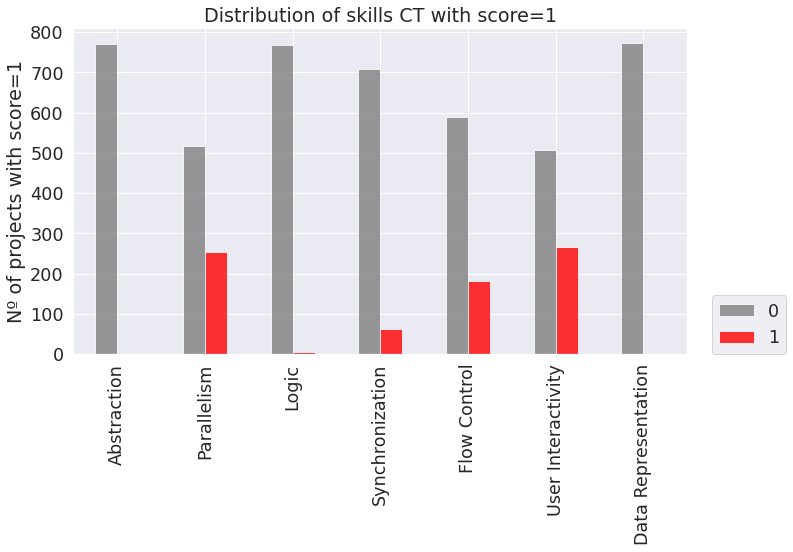
\includegraphics[width=\textwidth]{img/distribucion_1_Scratch}
        \caption{Diagrama de barras. Total=1}
        \label{fig:total1}
    \end{subfigure}       
    \begin{subfigure}[h]{.49\textwidth} 
        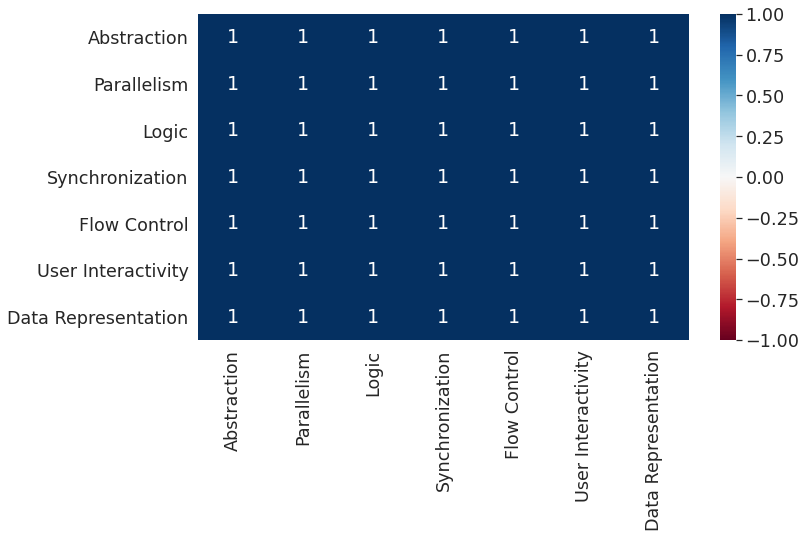
\includegraphics[width=\textwidth]{img/corr_1_Scratch}
        \caption{Matriz de correlación. Total=1}
        \label{fig:corr1}
    \end{subfigure}
     \caption{Distribución de puntuaciones y correlación entre dimensiones si el total es 1.}
\end{figure}

\begin{figure}[H]
    \centering
    \begin{subfigure}[h]{.49\textwidth} 
        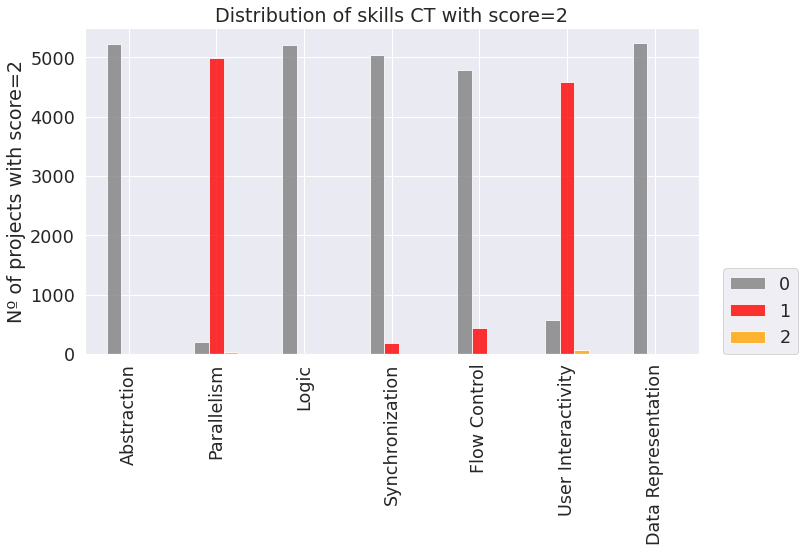
\includegraphics[width=\textwidth]{img/distribucion_2_Scratch}
        \caption{Diagrama de barras. Total=2}
        \label{fig:total2}
    \end{subfigure}       
    \begin{subfigure}[h]{.49\textwidth} 
        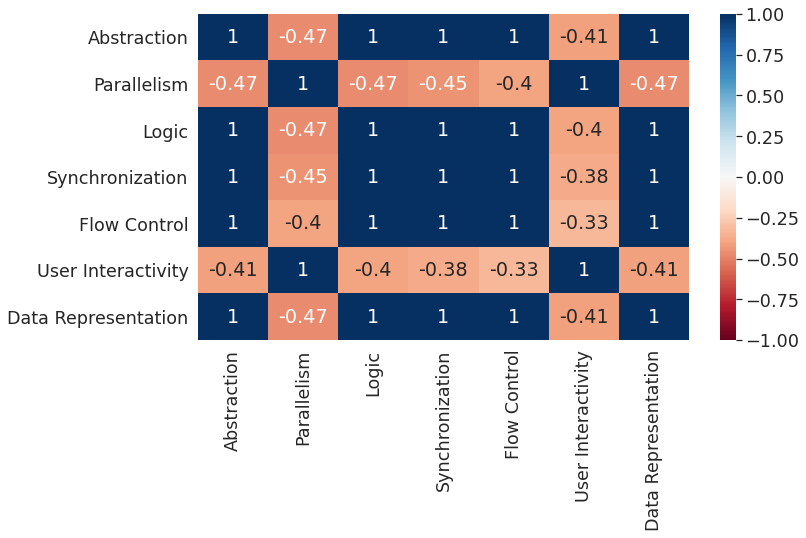
\includegraphics[width=\textwidth]{img/corr_2_Scratch}
        \caption{Matriz de correlación. Total=2}
        \label{fig:corr2}
    \end{subfigure}
     \caption{Distribución de puntuaciones y correlación entre dimensiones si el total es 2.}
\end{figure}

Como se percibe en la figura~\ref{fig:total2} la mayor parte de los proyectos cuentan con 1 punto en paralelismo y en interactividad con el usuario, que agregados conforman el total de 2.

De la matriz de correlación de la figura~\ref{fig:corr2} se deduce que aquellos pares de variables en los que la correlación no es perfecta y positiva, tienen una correlación débil y negativa. Entre paralelismo e interactividad con el usuario se produce una dependencia lineal perfecta, ya que cuando el usuario pulsa la bandera verde se desencadena la ejecución de varios flujos de código simultáneamente. Estas dos dimensiones se relacionan en sentido inverso con las otras aptitudes. El resto de dimensiones mantienen entre sí una relación perfecta positiva porque no puntúan. 

\begin{figure}[H]
    \centering
    \begin{subfigure}[h]{.49\textwidth} 
        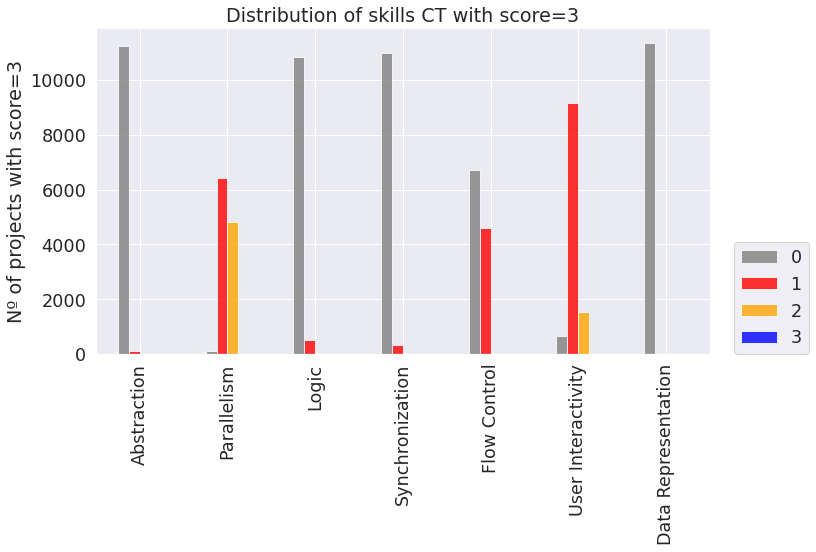
\includegraphics[width=\textwidth]{img/distribucion_3_Scratch}
        \caption{Diagrama de barras. Total=3}
        \label{fig:total3}
    \end{subfigure}       
    \begin{subfigure}[h]{.49\textwidth} 
        \includegraphics[width=\textwidth]{img/corr_3_Scratch}
        \caption{Matriz de correlación. Total=3}
        \label{fig:corr3}
    \end{subfigure}
     \caption{Distribución de puntuaciones y correlación entre dimensiones si el total es 3.}
\end{figure}

En la figura~\ref{fig:total3} se observa que los proyectos completan los 3 puntos totales con 1 o 2 puntos en paralelismo, 1 punto en interactividad con el usuario o incluso 1 punto en control de flujo, puesto que la frecuencia de ocurrencia es superior a 4.000.

Persisten las dependencias lineales positivas perfectas, con $\rho=1$, entre las capacidades con valoración nula, como se constata en la figura~\ref{fig:corr3}. Entre paralelismo e interactividad con el usuario hay una correlación positiva alta, igual que entre control de flujo y lógica y entre control de flujo y sincronización. No hay dependencia lineal entre control de flujo y paralelismo. Hay una correlación negativa moderada entre paralelismo con: representación de los datos, abstracción, lógica o sincronización. Es extraño que según aumenta una de las variables disminuya la otra, ya que el aumento en la capacidad para realizar tareas simultáneamente, no tiene por qué disminuir a la capacidad para establecer los atributos de los distintos objetos del proyecto o la habilidad para subdividir el problema en partes o ser capaz de establecer las condiciones que determinan la ejecución de unas acciones u otras. El hecho de que según aumenta paralelismo disminuya sincronización es bastante contradictorio, pues si se realizan tareas simultáneas debe existir alguna forma de que ajusten su ejecución en el tiempo.

En el diagrama de barras~\ref{fig:total4} se ve que en abstracción, lógica, sincronización y representación de los datos se siguen obteniendo 0 puntos en la mayoría de los proyectos. Sin embargo, se incrementan los que consiguen 1 punto en lógica, en sincronización y en control de flujo.

\begin{figure}[H]
    \centering
    \begin{subfigure}[h]{.49\textwidth} 
        \includegraphics[width=\textwidth]{img/distribucion_4_Scratch}
        \caption{Diagrama de barras. Total=4}
        \label{fig:total4}
    \end{subfigure}       
    \begin{subfigure}[h]{.49\textwidth} 
        \includegraphics[width=\textwidth]{img/corr_4_Scratch}
        \caption{Matriz de correlación. Total=4}
        \label{fig:corr4}
    \end{subfigure}
     \caption{Distribución de puntuaciones y correlación entre dimensiones si el total es 4.}
\end{figure}

En la matriz de correlación~\ref{fig:corr4} queda patente que existe dependencia lineal casi perfecta entre las dimensiones cuya puntuación más frecuente es 0 puntos. Cuando se codifican programas interactivos aumentan las nociones algorítmicas, como se deduce de la elevada relación lineal directa entre interactividad con el usuario y control de flujo. No existe dependencia lineal entre representación de los datos y control de flujo, ni entre este último y abstracción. Existe una correlación negativa moderada entre paralelismo y abstracción. El aumento de la valoración en una de las habilidades no debería hacer disminuir la otra. De hecho, la descomposición del programa en subprogramas encargados de tareas concretas podría facilitar la ejecución simultánea de varios subprogramas. También se da este tipo de correlación negativa entre paralelismo y representación de los datos.

Según el diagrama de barras~\ref{fig:total5} correspondiente a la puntuación total de 5, paralelismo e interactividad con el usuario son las capacidades mejor valoradas, puesto que la mitad de los proyectos consiguen 2 puntos. También aumenta la cantidad de proyectos que consiguen 1 punto en lógica y sincronización.

Al aumentar las puntuaciones, hay menos pares de dimensiones con coeficiente de correlación perfecto. Las máximas correlaciones en sentido positivo se producen entre paralelismo e interactividad con el usuario, y en menor medida entre representación de los datos y abstracción, entre sincronización y lógica y entre representación de los datos y lógica, como se observa en la figura~\ref{fig:corr5}. Resulta llamativo que no exista correlación entre sincronización y paralelismo, ya que si se ejecutan varios conjuntos de bloques a la vez tiene que existir algún evento que sincronice los procesos de manera que se comuniquen entre sí. Vuelve a aparecer una correlación moderada en sentido negativo entre paralelismo y abstracción con el mismo coeficiente que en la puntuación total de 4 puntos. También se obtiene una correlación de este tipo entre interactividad con el usuario y abstracción.

\begin{figure}[H]
    \centering
    \begin{subfigure}[h]{.49\textwidth} 
        \includegraphics[width=\textwidth]{img/distribucion_5_Scratch}
        \caption{Diagrama de barras. Total=5}
        \label{fig:total5}
    \end{subfigure}       
    \begin{subfigure}[h]{.49\textwidth} 
        \includegraphics[width=\textwidth]{img/corr_5_Scratch}
        \caption{Matriz de correlación. Total=5}
        \label{fig:corr5}
    \end{subfigure}
     \caption{Distribución de puntuaciones y correlación entre dimensiones si el total es 5.}
\end{figure}

Según se distingue en el diagrama de barras~\ref{fig:total6} correspondiente a la puntuación total de 6, se eleva la cantidad de proyectos con 1 punto en sincronización, control de flujo, interactividad con el usuario y representación de los datos.

Paralelismo y abstracción obtienen una correlación moderada en sentido negativo similar a la puntuación anterior. No hay correlación entre abstracción y sincronización, ni entre paralelismo y representación de los datos, como se aprecia en la matriz~\ref{fig:corr6}. Las mayores correlaciones se obtienen entre: control de flujo y sincronización, de modo que la secuenciación precisa, concreta y ordenada de instrucciones o bloques afecta a la organización temporal de los distintos flujos de código para que interactúen entre sí; entre lógica y representación de los datos, ya que tener una alta capacidad para buscar la solución al problema e implementar distintas acciones en función de condiciones, influye en almacenar en atributos y variables los datos tanto de condiciones como de resultados. Entre paralelismo e interactividad con el usuario existe una alta  dependencia ya que el usuario puede pulsar sobre una tecla u objeto provocando la ejecución simultánea de varias secuencias de bloques.%%

\begin{figure}[H]
    \centering
    \begin{subfigure}[h]{.49\textwidth} 
        \includegraphics[width=\textwidth]{img/distribucion_6_Scratch}
        \caption{Diagrama de barras. Total=6}
        \label{fig:total6}
    \end{subfigure}       
    \begin{subfigure}[h]{.49\textwidth} 
        \includegraphics[width=\textwidth]{img/corr_6_Scratch}
        \caption{Matriz de correlación. Total=6}
        \label{fig:corr6}
    \end{subfigure}
     \caption{Distribución de puntuaciones y correlación entre dimensiones si el total es 6.}
\end{figure}

Para la puntuación total de 7, lo más destacable en la representación de frecuencias de la figura~\ref{fig:total7} es que el número de proyectos con una puntuación de 2 en paralelismo aumenta.

La correlación es perfecta positiva entre control de flujo y sincronización y entre lógica y representación de los datos, como se visualiza en la matriz~\ref{fig:corr7}. Se alcanzan valores elevados entre lógica y sincronización, representación de los datos y sincronización, control de flujo y lógica, interactividad con el usuario y control de flujo y entre interactividad con el usuario y sincronización. Que no exista correlación entre sincronización y paralelismo resulta contradictorio, ya que si se ejecutan flujos de código a la vez debería desarrollarse la capacidad de sincronizarlos, aunque no precisamente con el bloque de espera evaluado con 1 punto. Tampoco existe correlación entre abstracción y representación de los datos, puesto que aún no se ha desarrollado la capacidad de dividir el problema en partes más simples.

\begin{figure}[H]
    \centering
    \begin{subfigure}[h]{.49\textwidth} 
        \includegraphics[width=\textwidth]{img/distribucion_7_Scratch}
        \caption{Diagrama de barras. Total=7}
        \label{fig:total7}
    \end{subfigure}       
    \begin{subfigure}[h]{.49\textwidth} 
        \includegraphics[width=\textwidth]{img/corr_7_Scratch}
        \caption{Matriz de correlación. Total=7}
        \label{fig:corr7}
    \end{subfigure}
     \caption{Distribución de puntuaciones y correlación entre dimensiones si el total es 7.}
\end{figure}

Cuando el total es 8, en interactividad con el usuario predominan los 2 puntos, mientras que en abstracción las puntuaciones siguen siendo bajas, como se ve en el diagrama de barras~\ref{fig:total8}.

En la matriz de correlación~\ref{fig:corr8} se obtiene de nuevo una casi perfecta correlación directa entre control de flujo y sincronización. También se consigue una correlación muy alta y en sentido positivo entre paralelismo e interactividad con el usuario, entre control de flujo y representación de los datos, entre sincronización y representación de los datos, así como entre lógica y abstracción. Sincronización y paralelismo vuelven a ser independientes linealmente. Tampoco existe correlación entre abstracción y sincronización, ni entre paralelismo y representación de los datos, de modo que la codificación de scripts para su ejecución simultánea no se ve afectada por la declaración y modificación de atributos y variables que simplifiquen el tratamiento de datos en los scripts, ni entre  interactividad con el usuario y pensamiento lógico, por lo que la implementación de distintas alternativas según se cumpla una condición no está sujeta a los eventos provocados por quién pruebe el proyecto. Se consigue de nuevo una correlación moderada en sentido negativo entre paralelismo y abstracción.% cambios de estado 

\begin{figure}[H]
    \centering
    \begin{subfigure}[h]{.49\textwidth} 
        \includegraphics[width=\textwidth]{img/distribucion_8_Scratch}
        \caption{Diagrama de barras. Total=8}
        \label{fig:total8}
    \end{subfigure}       
    \begin{subfigure}[h]{.49\textwidth} 
        \includegraphics[width=\textwidth]{img/corr_8_Scratch}
        \caption{Matriz de correlación. Total=8}
        \label{fig:corr8}
    \end{subfigure}
     \caption{Distribución de puntuaciones y correlación entre dimensiones si el total es 8.}
\end{figure}

Para la puntuación total de 9, en la matriz de correlación~\ref{fig:corr9} se observan valores elevados próximos a 1, que indican correlación casi perfecta, en lógica con representación de los datos, en paralelismo con interactividad con el usuario, en control de flujo con representación de los datos y en control de flujo con sincronización. Las correlaciones entre sincronización con lógica y entre control de flujo con lógica son menores pero también elevadas. Sigue sin existir correlación entre control de flujo y abstracción, entre sincronización y abstracción, entre sincronización y paralelismo y entre lógica y paralelismo. Se vuelve además a obtener una correlación negativa moderada entre paralelismo y abstracción similar a la conseguida en puntuaciones anteriores, aún cuando se incrementa la destreza en abstracción, como se ve en el diagrama~\ref{fig:total9}.

\begin{figure}[H]
    \centering
    \begin{subfigure}[h]{.49\textwidth} 
        \includegraphics[width=\textwidth]{img/distribucion_9_Scratch}
        \caption{Diagrama de barras. Total=9}
        \label{fig:total9}
    \end{subfigure}       
    \begin{subfigure}[h]{.49\textwidth} 
        \includegraphics[width=\textwidth]{img/corr_9_Scratch}
        \caption{Matriz de correlación. Total=9}
        \label{fig:corr9}
    \end{subfigure}
     \caption{Distribución de puntuaciones y correlación entre dimensiones si el total es 9.}
\end{figure}

Para la puntuación total de 10, en el diagrama de barras~\ref{fig:total10} aumenta la obtención de 2 puntos en lógica y de 3 puntos en representación de los datos, por el uso de listas. 

Existe una correlación perfecta directa entre lógica y paralelismo. Se consigue también una alta correlación positiva entre lógica e interactividad con el usuario y entre esta última y paralelismo. No hay dependencia lineal entre control de flujo y abstracción, ni entre sincronización y lógica, ni entre sincronización y paralelismo. Igual que en la puntuación anterior se obtiene una correlación moderada en sentido negativo entre abstracción y paralelismo. La capacidad de dividir el problema en partes sencillas de implementar y depurar, debería ayudar a descubrir cuáles de estas partes pueden ser ejecutadas de manera simultánea o concurrente, con una adecuada sincronización. Sin embargo el aumento de una habilidad hace que disminuya la otra. Además ambas son independientes de sincronización puesto que solo se usan bloques de espera. 

\begin{figure}[H]
    \centering
    \begin{subfigure}[h]{.49\textwidth} 
        \includegraphics[width=\textwidth]{img/distribucion_10_Scratch}
        \caption{Diagrama de barras. Total=10}
        \label{fig:total10}
    \end{subfigure}       
    \begin{subfigure}[h]{.49\textwidth} 
        \includegraphics[width=\textwidth]{img/corr_10_Scratch}
        \caption{Matriz de correlación. Total=10}
        \label{fig:corr10}
    \end{subfigure}
     \caption{Distribución de puntuaciones y correlación entre dimensiones si el total es 10.}
\end{figure}

Para la puntuación total de 11, en el diagrama de barras~\ref{fig:total11} destaca el aumento de proyectos que consiguen 3 puntos en pensamiento lógico.

En la matriz de correlación~\ref{fig:corr11} se observan valores elevados entre interactividad con el usuario y paralelismo, entre sincronización y representación de los datos y entre control de flujo con interactividad con el usuario. Son independientes linealmente: control de flujo y abstracción, representación de los datos y abstracción, lógica y representación de los datos, lógica y control de flujo, interactividad del usuario y representación de los datos. Vuelve a existir correlación en sentido negativo entre paralelismo y abstracción. También se da una correlación negativa prácticamente perfecta entre lógica y abstracción. Al aumentar el uso de estructuras selectivas que pueden incluir operadores lógicos, disminuye la capacidad para plantear soluciones a problemas descomponiéndolos en scripts o funciones encargadas de tareas concretas que pueden ser reutilizadas cuando se extrae lo relevante, se reconocen patrones y se generaliza. % Evolución de la programación estructurada a la modular.

\begin{figure}[H]
    \centering
    \begin{subfigure}[h]{.49\textwidth} 
        \includegraphics[width=\textwidth]{img/distribucion_11_Scratch}
        \caption{Diagrama de barras. Total=11}
        \label{fig:total11}
    \end{subfigure}       
    \begin{subfigure}[h]{.49\textwidth} 
        \includegraphics[width=\textwidth]{img/corr_11_Scratch}
        \caption{Matriz de correlación. Total=11}
        \label{fig:corr11}
    \end{subfigure}
     \caption{Distribución de puntuaciones y correlación entre dimensiones si el total es 11.}
\end{figure}

Para la puntuación de 12, según la matriz~\ref{fig:corr12}, existe una correlación elevada directa entre lógica y paralelismo, y entre paralelismo e interactividad con el usuario. Por ello cuando el usuario pulsa una tecla o un objeto se desencadena la ejecución de varias tareas a la vez. Se da una correlación positiva menor entre sincronización y abstracción y entre interactividad con el usuario y lógica. No hay correlación entre sincronización e interactividad con el usuario. La correlación en sentido negativo entre paralelismo y abstracción se aproxima a -1, mientras que entre lógica y abstracción es fuerte pero no perfecta, comparada con la puntuación anterior. 

\begin{figure}[H]
    \centering
    \begin{subfigure}[h]{.49\textwidth} 
        \includegraphics[width=\textwidth]{img/distribucion_12_Scratch}
        \caption{Diagrama de barras. Total=12}
        \label{fig:total12}
    \end{subfigure}       
    \begin{subfigure}[h]{.49\textwidth} 
        \includegraphics[width=\textwidth]{img/corr_12_Scratch}
        \caption{Matriz de correlación. Total=12}
        \label{fig:corr12}
    \end{subfigure}
     \caption{Distribución de puntuaciones y correlación entre dimensiones si el total es 12.}
\end{figure}

Para la puntuación total de 13, el diagrama de barras~\ref{fig:total13} refleja un aumento en el uso de clones o instancias de los personajes creadas dinámicamente con el mismo comportamiento que el objeto inicial, como se infiere de la cantidad de proyectos con 3 puntos en abstracción.

En la matriz~\ref{fig:corr13} se obtiene una correlación positiva fuerte entre sincronización y abstracción, entre paralelismo e interactividad con el usuario, entre lógica y paralelismo 
y entre representación de los datos y abstracción. Al declarar atributos y listas y modificar su contenido se abstraen características de los personajes y se agrupan datos que pueden ser procesados por una misma secuencia de instrucciones o programa. No existe dependencia lineal entre interactividad del usuario con sincronización, entre control de flujo y representación de los datos, ni entre lógica y abstracción.

\begin{figure}[H]
    \centering
    \begin{subfigure}[h]{.49\textwidth} 
        \includegraphics[width=\textwidth]{img/distribucion_13_Scratch}
        \caption{Diagrama de barras. Total=13}
        \label{fig:total13}
    \end{subfigure}       
    \begin{subfigure}[h]{.49\textwidth} 
        \includegraphics[width=\textwidth]{img/corr_13_Scratch}
        \caption{Matriz de correlación. Total=13}
        \label{fig:corr13}
    \end{subfigure}
     \caption{Distribución de puntuaciones y correlación entre dimensiones si el total es 13.}
\end{figure}

Para la puntuación total de 14, en el diagrama de barras~\ref{fig:total14} la puntuación más frecuente en lógica es 3. En los proyectos que la consiguen 
se evalúan varias situaciones utilizando operadores lógicos, que permiten elegir entre distintas alternativas, obteniendo salidas diferentes.

En la matriz~\ref{fig:corr14} se observa una correlación positiva casi perfecta entre control de flujo e interactividad con el usuario. La dependencia lineal es elevada y positiva entre: paralelismo e interactividad con el usuario, representación de los datos con abstracción, control de flujo con paralelismo y lógica con paralelismo. Interactividad del usuario y sincronización son incorreladas, indicando que la gestión de las respuestas del usuario ante determinadas preguntas, de los movimientos con el ratón sobre objetos o de cómo responde el programa cuando se pulsa una tecla, no afecta a la capacidad del programador para planificar el orden en que se ejecutan las distintas tareas de modo que interactúen entre sí.

\begin{figure}[H]
    \centering
    \begin{subfigure}[h]{.49\textwidth} 
        \includegraphics[width=\textwidth]{img/distribucion_14_Scratch}
        \caption{Diagrama de barras. Total=14}
        \label{fig:total14}
    \end{subfigure}       
    \begin{subfigure}[h]{.49\textwidth} 
        \includegraphics[width=\textwidth]{img/corr_14_Scratch}
        \caption{Matriz de correlación. Total=14}
        \label{fig:corr14}
    \end{subfigure}
     \caption{Distribución de puntuaciones y correlación entre dimensiones si el total es 14.}
\end{figure}

Con respecto a la puntuación total de 15, en el diagrama de barras~\ref{fig:total15} se percibe un incremento en las frecuencias correspondientes a los 3 puntos tanto en abstracción, al emplear clones, como en representación de los datos, por utilizar listas.

La matriz de correlación~\ref{fig:corr15} muestra una dependencia lineal directa perfecta entre control de flujo con interactividad con el usuario, y una correlación positiva muy elevada entre lógica y abstracción, entre representación de los datos y abstracción, entre lógica y paralelismo, entre interactividad con el usuario y paralelismo y entre control de flujo y paralelismo. Como en otras puntuaciones anteriores, sincronización e interactividad con el usuario, abstracción e interactividad con el usuario y control de flujo y sincronización están incorreladas.

\begin{figure}[H]
    \centering
    \begin{subfigure}[h]{.49\textwidth} 
        \includegraphics[width=\textwidth]{img/distribucion_15_Scratch}
        \caption{Diagrama de barras. Total=15}
        \label{fig:total15}
    \end{subfigure}       
    \begin{subfigure}[h]{.49\textwidth} 
        \includegraphics[width=\textwidth]{img/corr_15_Scratch}
        \caption{Matriz de correlación. Total=15}
        \label{fig:corr15}
    \end{subfigure}
     \caption{Distribución de puntuaciones y correlación entre dimensiones si el total es 15.}
\end{figure}

En la puntuación total de 16 se consigue que la máxima puntuación sea la más frecuente en abstracción, \emph{lógica} y representación de los datos. En paralelismo, control de flujo e interactividad con el usuario persisten los 2 puntos, como se constata en el diagrama~\ref{fig:total16}.

Según la figura~\ref{fig:corr16} se producen elevadas dependencias en sentido positivo, ordenadas de mayor a menor, entre interactividad del usuario y control de flujo, entre lógica y paralelismo, entre abstracción y representación de los datos, entre lógica y abstracción y entre paralelismo y abstracción. La dependencia lineal de este último par ha cambiado de sentido con respecto a las 12 primeras puntuaciones totales, de manera que al aumentar la capacidad para dar modularidad al código y utilizar clones, se incrementa la habilidad de discernir qué funciones y procedimientos pueden ejecutarse simultáneamente cuando se produzca un evento. No existe correlación entre control de flujo y sincronización, ni entre interactividad del usuario y sincronización, ni entre control de flujo y abstracción, ni entre interactividad del usuario y abstracción, ni entre paralelismo y sincronización, ni entre lógica y sincronización. 

\begin{figure}[H]
    \centering
    \begin{subfigure}[h]{.49\textwidth} 
        \includegraphics[width=\textwidth]{img/distribucion_16_Scratch}
        \caption{Diagrama de barras. Total=16}
        \label{fig:total16}
    \end{subfigure}       
    \begin{subfigure}[h]{.49\textwidth} 
        \includegraphics[width=\textwidth]{img/corr_16_Scratch}
        \caption{Matriz de correlación. Total=16}
        \label{fig:corr16}
    \end{subfigure}
     \caption{Distribución de puntuaciones y correlación entre dimensiones si el total es 16.}
\end{figure}

Con respecto a la puntuación total de 17, mientras que abstracción, paralelismo, lógica y representación de datos están prácticamente desarrolladas, control de flujo e interactividad del usuario se mantienen en los 2 puntos, como se aprecia en la figura~\ref{fig:total17}. La cantidad de proyectos de Scratch que consiguen 1 y 3 puntos en sincronización es similar.

Según se muestra en la matriz de correlación~\ref{fig:corr17}
se establecen interdependencias lineales perfectas directas entre las capacidades con 3 puntos, de manera que al descomponer en partes más sencillas el problema definiendo funciones propias o creando dinámicamente clones de los personajes, 
se ejecutan simultáneamente varios flujos de código o programas y en algunos de ellos se emplean condicionales con operadores lógicos para decidir el conjunto de instrucciones a ejecutar y cómo se modifican los datos contenidos en listas.
No existe dependencia lineal entre control de flujo y abstracción, entre control de flujo y sincronización, ni entre interactividad del usuario y la mayor parte de las dimensiones, salvo control de flujo, porque cuando se crean programas interactivos aumenta la capacidad de diseñar y aplicar algoritmos iterativos.

\begin{figure}[H]
    \centering
    \begin{subfigure}[h]{.49\textwidth} 
        \includegraphics[width=\textwidth]{img/distribucion_17_Scratch}
        \caption{Diagrama de barras. Total=17}
        \label{fig:total17}
    \end{subfigure}       
    \begin{subfigure}[h]{.49\textwidth} 
        \includegraphics[width=\textwidth]{img/corr_17_Scratch}
        \caption{Matriz de correlación. Total=17}
        \label{fig:corr17}
    \end{subfigure}
     \caption{Distribución de puntuaciones y correlación entre dimensiones si el total es 17.}
\end{figure}

El paso de los 17 a los 18 puntos totales está marcado por el desarrollo casi completo de la sincronización, como se deduce al comparar los diagramas de barras~\ref{fig:total17} y ~\ref{fig:total18}.

\begin{figure}[H]
    \centering
    \begin{subfigure}[h]{.49\textwidth} 
        \includegraphics[width=\textwidth]{img/distribucion_18_Scratch}
        \caption{Diagrama de barras. Total=18}
        \label{fig:total18}
    \end{subfigure}       
    \begin{subfigure}[h]{.49\textwidth} 
        \includegraphics[width=\textwidth]{img/corr_18_Scratch}
        \caption{Matriz de correlación. Total=18}
        \label{fig:corr18}
    \end{subfigure}
     \caption{Distribución de puntuaciones y correlación entre dimensiones si el total es 18.}
\end{figure}

Se conservan las correlaciones casi perfectas explicadas en la puntuación anterior y se añaden las que surgen entre sincronización con las otras habilidades evaluadas con 3 puntos. Por ello cuando se establece previamente el orden en que los programas serán ejecutados, de forma que interactúen y se comuniquen entre sí con mensajes, eventos o esperando el resultado de algún script, resulta más fácil que las distintas partes en que se descompone el problema puedan ejecutarse en paralelo, empleen estructuras selectivas que indiquen por donde continúa el flujo del programa y se utilicen métodos propios de listas para modificar los datos que contiene, que a su vez pueden ser usados como condiciones o eventos. Existe una correlación positiva baja entre control de flujo y lógica. Entre cada par de variables no comentadas, se puede decir que no existe correlación. Todo esto queda reflejado en la matriz~\ref{fig:corr18}.

\begin{figure}[H]
    \centering
    \begin{subfigure}[h]{.49\textwidth} 
        \includegraphics[width=\textwidth]{img/distribucion_19_Scratch}
        \caption{Diagrama de barras. Total=19}
        \label{fig:total19}
    \end{subfigure}       
    \begin{subfigure}[h]{.49\textwidth} 
        \includegraphics[width=\textwidth]{img/corr_19_Scratch}
        \caption{Matriz de correlación. Total=19}
        \label{fig:corr19}
    \end{subfigure}
     \caption{Distribución de puntuaciones y correlación entre dimensiones si el total es 19.}
\end{figure}

Cuando la complejidad de los proyectos alcanza los 19 puntos, control de flujo e interactividad con el usuario siguen en 2 puntos, y el resto de dimensiones se perfilan aún más en los 3 puntos, marcando un desarrollo completo (ver figura~\ref{fig:total19}).

Debido a esta distribución de puntuaciones, las matrices de correlación~\ref{fig:corr18} y~\ref{fig:corr19} muestran las mismas correlaciones perfectas positivas. Control de flujo es independiente linealmente de las otras dimensiones, salvo de interactividad con el usuario. Interactividad con el usuario presenta correlaciones inversas bajas y moderadas con el resto  de dimensiones.

Para la puntuación total de 20, control de flujo logra alcanzar la máxima puntuación al utilizarse bucles en donde se itera hasta que se cumple una condición.

La correlación es perfecta positiva entre todas las dimensiones del pensamiento computacional, salvo para interactividad con el usuario con el resto de dimensiones, como vemos en la matriz~\ref{fig:corr20}. Esto se debe a que, según vemos en el diagrama de barras~\ref{fig:total20}, las puntuaciones de la mayor parte de los proyectos para interactividad con el usuario son de 2 puntos. Por ello su correlación es perfecta negativa con cada una de las otras áreas del PC. 

\begin{figure}[H]
    \centering
    \begin{subfigure}[h]{.49\textwidth} 
        \includegraphics[width=\textwidth]{img/distribucion_20_Scratch}
        \caption{Diagrama de barras. Total=20}
        \label{fig:total20}
    \end{subfigure}       
    \begin{subfigure}[h]{.49\textwidth} 
        \includegraphics[width=\textwidth]{img/corr_20_Scratch}
        \caption{Matriz de correlación. Total=20}
        \label{fig:corr20}
    \end{subfigure}
     \caption{Distribución de puntuaciones y correlación entre dimensiones si el total es 20.}
\end{figure}

Por lo tanto la última dimensión en desarrollarse por completo es interactividad con el usuario. El cambio de los 2 a los 3 puntos se produce por implementar acciones en los personajes que respondan a las modificaciones en el audio y el vídeo que realiza el usuario para interactuar con el proyecto de Scratch, aunque en el conjunto de proyectos analizado no se aplica demasiado.

\section{Población de proyectos de Snap!}
\label{append_Snap}

Los proyectos más simples evaluados con 1 punto consiguen esta valoración principalmente por el desarrollo de la abstracción, como se demuestra en el diagrama de barras~\ref{fig:total1_Snap}. Llama la atención que la descomposición del problema en partes sencillas sea la primera habilidad en manifestarse. Estos proyectos contienen funciones definidas por el programador, varios scripts que resuelven subproblemas bien definidos y varios personajes u objetos cada uno con sus propios atributos y programas o clones que son instancias de los objetos. 

En la matriz de correlación~\ref{fig:corr1_Snap} las dependencias lineales son perfectas positivas entre cada par de dimensiones con valores nulos, salvo en abstracción con el resto de dimensiones, donde es perfecta negativa.

\begin{figure}[H]
    \centering
    \begin{subfigure}[h]{.49\textwidth} 
        \includegraphics[width=\textwidth]{img/distribucion_1_Snap}
        \caption{Diagrama de barras. Total=1}
        \label{fig:total1_Snap}
    \end{subfigure}       
    \begin{subfigure}[h]{.49\textwidth} 
        \includegraphics[width=\textwidth]{img/corr_1_Snap}
        \caption{Matriz de correlación. Total=1}
        \label{fig:corr1_Snap}
    \end{subfigure}
     \caption{Snap!: Distribución de valores y correlación entre dimensiones si el total es 1.}
\end{figure}

Como se distingue en la distribución~\ref{fig:total2_Snap}, la puntuación total de 2 se obtiene de las distintas combinaciones del punto conseguido en control de flujo, interactividad con el usuario o abstracción. Entre estas dos últimas se da una correlación positiva casi perfecta. Control de flujo muestra una correlación positiva alta con el resto de dimensiones, mientras que en interactividad con el usuario y abstracción no existe correlación con las habilidades no desarrolladas. Estas dimensiones que no puntúan presentan entre sí correlaciones positivas perfectas, como se ve en la matriz~\ref{fig:corr2_Snap}.

\begin{figure}[H]
    \centering
    \begin{subfigure}[h]{.49\textwidth} 
        \includegraphics[width=\textwidth]{img/distribucion_2_Snap}
        \caption{Diagrama de barras. Total=2}
        \label{fig:total2_Snap}
    \end{subfigure}       
    \begin{subfigure}[h]{.49\textwidth} 
        \includegraphics[width=\textwidth]{img/corr_2_Snap}
        \caption{Matriz de correlación. Total=2}
        \label{fig:corr2_Snap}
    \end{subfigure}
     \caption{Snap!: Distribución de valores y correlación entre dimensiones si el total es 2.}
\end{figure}

Aumenta la cantidad de proyectos que consiguen puntuar en representación de los datos y se consigue una ligera mejora en control de flujo, como se distingue en la distribución~\ref{fig:total3_Snap}.

Según la matriz~\ref{fig:corr3_Snap}, en esta puntuación total de 3, surgen altas interdependencias directas entre cada dimensión con interactividad con el usuario, excluyendo control de flujo. Que el usuario presione la bandera verde o una tecla no guarda relación con una secuenciación finita, ordenada y precisa de las instrucciones que penden de esos bloques de inicialización del programa. En cambio sí depende de la resolución del problemas dividiéndolo en funciones o procedimientos encargados de una tarea determinada o empleando instancias de los personajes, propias de la abstracción, o de la modificación de los datos que caracterizan a cada personaje. Representación de los datos también se relaciona fuertemente con control de flujo y abstracción. Sincronización, condicionales y paralelismo siguen sin puntuar y presentan entre sí correlaciones perfectas directas, siendo independientes de control de flujo.

\begin{figure}[H]
    \centering
    \begin{subfigure}[h]{.49\textwidth} 
        \includegraphics[width=\textwidth]{img/distribucion_3_Snap}
        \caption{Diagrama de barras. Total=3}
        \label{fig:total3_Snap}
    \end{subfigure}       
    \begin{subfigure}[h]{.49\textwidth} 
        \includegraphics[width=\textwidth]{img/corr_3_Snap}
        \caption{Matriz de correlación. Total=3}
        \label{fig:corr3_Snap}
    \end{subfigure}
     \caption{Snap!: Distribución de valores y correlación entre dimensiones si el total es 3.}
\end{figure}

Las diferencias del diagrama de barras~\ref{fig:total4_Snap} correspondiente a la puntuación total de 4 con respecto al anterior, son mayores frecuencias para el punto obtenido en paralelismo e interactividad y para los 2 puntos en control de flujo.

Paralelismo mantiene correlaciones positivas perfectas con sincronización y condicionales, pese a que sea la única que progresa con respecto a las otras dos. Establece con abstracción una dependencia lineal fuerte en sentido positivo. Por ello aumenta la capacidad para ejecutar programas y funciones de manera simultánea cuando el problema se resuelve dividiéndolo en módulos más sencillos de codificar. 
La misma dependencia surge entre interactividad con el usuario y representación de los datos, de forma que cuando el evento que provoca el usuario ocurre, se incrementan las operaciones sobre los atributos de los objetos. 
Abstracción y control de flujo son independientes, las copias de los personajes, y los scripts o bloques encargados de tareas concretas que resuelven el problema en su conjunto, no influye en que se demuestren nociones algorítmicas en su codificación.
Tampoco hay correlación entre condicionales con representación de los datos, ni entre esta última con sincronización. La ausencia tanto de condicionales como de sincronización no afecta a la capacidad de definir los atributos de los personajes que necesitan los programas, que se van modificando durante su ejecución.

\begin{figure}[H]
    \centering
    \begin{subfigure}[h]{.49\textwidth} 
        \includegraphics[width=\textwidth]{img/distribucion_4_Snap}
        \caption{Diagrama de barras. Total=4}
        \label{fig:total4_Snap}
    \end{subfigure}       
    \begin{subfigure}[h]{.49\textwidth} 
        \includegraphics[width=\textwidth]{img/corr_4_Snap}
        \caption{Matriz de correlación. Total=4}
        \label{fig:corr4_Snap}
    \end{subfigure}
     \caption{Snap!: Distribución de valores y correlación entre dimensiones si el total es 4.}
\end{figure}

En la distribución~\ref{fig:total5_Snap}, cuando se filtra para un nivel de complejidad total de 5, los proyectos con 2 puntos prevalecen en control de flujo. En sincronización aumenta la cantidad de proyectos que consiguen 1 punto, si bien la mayoría no puntúan.

\begin{figure}[H]
    \centering
    \begin{subfigure}[h]{.49\textwidth} 
        \includegraphics[width=\textwidth]{img/distribucion_5_Snap}
        \caption{Diagrama de barras. Total=5}
        \label{fig:total5_Snap}
    \end{subfigure}       
    \begin{subfigure}[h]{.49\textwidth} 
        \includegraphics[width=\textwidth]{img/corr_5_Snap}
        \caption{Matriz de correlación. Total=5}
        \label{fig:corr5_Snap}
    \end{subfigure}
    \caption{Snap!: Distribución de valores y correlación entre dimensiones si el total es 5.}
\end{figure}

En la matriz~\ref{fig:corr5_Snap} se mantiene una correlación perfecta entre sincronización y condicionales. Asimismo, son muy elevadas las dependencias lineales directas entre cada par conformado por abstracción, sincronización y paralelismo. Se descompone el problema en tareas más simples y en personajes para los que se ha establecido un orden temporal en el que ejecutar las distintas acciones de manera concurrente o simultánea, pudiendo interactuar entre sí. El usuario provoca que los objetos ejecuten esos procesos a la vez al pulsar una tecla o cambiando el estado del objeto, modificando las propiedades del objeto, ya sea su posición, disfraz o movimiento, generando altas dependencias entre interactividad con: abstracción, paralelismo y representación de los datos. Sin embargo, sincronización y representación de los datos están incorreladas. Se produce una correlación moderada negativa entre control de flujo y condicionales. 

En la distribución~\ref{fig:total6_Snap} la proporción de proyectos con 1 punto en sincronización, paralelismo e interactividad con el usuario se eleva. En menor medida, se consiguen 2 puntos en estas dos últimas, así como en abstracción. Incluso se obtienen 3 puntos al emplear estructuras de datos complejas como entrada de sus programas.

En la matriz~\ref{fig:corr6_Snap} de nuevo se presentan las mismas dependencias casi perfectas entre sincronización y condicionales, interactividad con el usuario y datos, abstracción con paralelismo y abstracción con sincronización. No se producen asociaciones entre interactividad con el usuario con condicionales, representación de los datos con condicionales, sincronización con representación de los datos, ni entre abstracción con control de flujo. Sigue dándose una correlación moderada negativa entre control de flujo con condicionales, de manera que al demostrar nociones algorítmicas por el uso de estructuras iterativas, se reducen los condicionales que permiten obtener distintas salidas según se cumpla o no una situación o un conjunto de ellas.

\begin{figure}[H]
    \centering
    \begin{subfigure}[h]{.49\textwidth} 
        \includegraphics[width=\textwidth]{img/distribucion_6_Snap}
        \caption{Diagrama de barras. Total=6}
        \label{fig:total6_Snap}
    \end{subfigure}       
    \begin{subfigure}[h]{.49\textwidth} 
        \includegraphics[width=\textwidth]{img/corr_6_Snap}
        \caption{Matriz de correlación. Total=6}
        \label{fig:corr6_Snap}
    \end{subfigure}
    \caption{Snap!: Distribución de valores y correlación entre dimensiones si el total es 6.}
\end{figure}

En el diagrama de barras~\ref{fig:total7_Snap} disminuye la habilidad demostrada en sincronización, mientras que trasciende abstracción. En paralelismo se igualan los proyectos con 1 y 2 puntos.

En la matriz de correlación~\ref{fig:corr7_Snap} de la puntuación global de 7, sincronización y condicionales son totalmente interdependientes entre sí puesto que apenas consiguen puntuar. Se conserva una correlación elevada entre interactividad con el usuario y representación de los datos y se obtienen además dependencias lineales elevadas entre cada una de ellas con abstracción. Al dividir la resolución del problema en partes mediante objetos o personajes, bloques personalizados o scripts con una funcionalidad muy concreta más fácil de programar y mantener, o con clones, se modifican y almacenan los datos que requieren en listas, variables, o atributos de los objetos y a su vez se gestionan los eventos causados por el usuario. Paralelismo y control de flujo están fuertemente correladas. Implica que si un personaje realiza varias acciones a la vez o varios personajes ejecutan simultáneamente el mismo código, se incrementa la capacidad de que cada programa siga una estructura secuencial o iterativa. No existe correlación entre paralelismo con condicionales, ni entre paralelismo con sincronización. La correlación negativa más remarcable es la que ocurre entre control de flujo con condicionales, que también se produce en las puntuaciones totales anteriores.

\begin{figure}[H]
    \centering
    \begin{subfigure}[h]{.49\textwidth} 
        \includegraphics[width=\textwidth]{img/distribucion_7_Snap}
        \caption{Diagrama de barras. Total=7}
        \label{fig:total7_Snap}
    \end{subfigure}       
    \begin{subfigure}[h]{.49\textwidth} 
        \includegraphics[width=\textwidth]{img/corr_7_Snap}
        \caption{Matriz de correlación. Total=7}
        \label{fig:corr7_Snap}
    \end{subfigure}
    \caption{Snap!: Distribución de valores y correlación entre dimensiones si el total es 7.}
\end{figure}

En la puntuación total de 8 el uso de condicionales adquiere mayor relevancia y cerca de unos 1.000 proyectos consiguen la máxima puntuación en paralelismo y control de flujo. En interactividad con el usuario y representación de los datos se incrementan los proyectos con 2 puntos, como se aprecia en el gráfico~\ref{fig:total8_Snap}.

En la matriz~\ref{fig:corr8_Snap} se observan correlaciones positivas muy altas entre interactividad con el usuario y representación de los datos, y entre ambas con control de flujo, de forma que se desencadena la ejecución de secuencias y ciclos de sentencias que modifican los atributos de los objetos y los datos contenidos en listas y variables cuando el usuario responde a una pregunta, pulsa una tecla o mueve un objeto con el ratón. Sincronización y condicionales también son interdependientes, pues cuando se codifican sentencias alternativas en función de condiciones, se planifica la interacción de los distintos procesos con bloques de parada, espera e intercambio de mensajes. Interactividad con el usuario y sincronización están incorreladas.

\begin{figure}[H]
    \centering
    \begin{subfigure}[h]{.49\textwidth} 
        \includegraphics[width=\textwidth]{img/distribucion_8_Snap}
        \caption{Diagrama de barras. Total=8}
        \label{fig:total8_Snap}
    \end{subfigure}       
    \begin{subfigure}[h]{.49\textwidth} 
        \includegraphics[width=\textwidth]{img/corr_8_Snap}
        \caption{Matriz de correlación. Total=8}
        \label{fig:corr8_Snap}
    \end{subfigure}
    \caption{Snap!: Distribución de valores y correlación entre dimensiones si el total es 8.}
\end{figure}

Como se aprecia en el diagrama~\ref{fig:total9_Snap}, si el total es 9 puntos, la sincronización alcanza un nivel intermedio, aumentando a la vez la cantidad de proyectos con un desarrollo avanzado en paralelismo y control de flujo. 

En la matriz ~\ref{fig:corr9_Snap} se constata que control de flujo presenta una elevada correlación directa con cada una de las siguientes: paralelismo, interactividad con el usuario y representación de los datos. 
Los programas codificados en base a una correcta secuenciación de pasos que pueden incluir bucles, demuestran nociones algorítmicas que facilitan dividir el problema en un conjunto de tareas que se realizan simultáneamente, que puedan ejecutarse cuando el usuario cambia el estado de un objeto y se modifiquen sus atributos o se empleen variables o listas como elemento abstracto para manejar los datos sobre los que operan estos programas. 

Abstracción es fuertemente interdependiente tanto con interactividad como con representación de los datos. Cuando el usuario controla el programa por teclado o por ratón se gestionan las acciones con clones, scripts o funciones propias, que emplean variables y listas para extraer patrones y generalizar a partir de scripts con una funcionalidad similar. Abstracción y sincronización son independientes entre sí. Existe una dependencia lineal moderada inversa entre control de flujo y condicionales y es aún más fuerte entre paralelismo y condicionales.

\begin{figure}[H]
    \centering
    \begin{subfigure}[h]{.49\textwidth} 
        \includegraphics[width=\textwidth]{img/distribucion_9_Snap}
        \caption{Diagrama de barras. Total=9}
        \label{fig:total9_Snap}
    \end{subfigure}       
    \begin{subfigure}[h]{.49\textwidth} 
        \includegraphics[width=\textwidth]{img/corr_9_Snap}
        \caption{Matriz de correlación. Total=9}
        \label{fig:corr9_Snap}
    \end{subfigure}
    \caption{Snap!: Distribución de valores y correlación entre dimensiones si el total es 9.}
\end{figure}

Cuando el total asciende a los 10 puntos, tanto en sincronización como en control de flujo la moda se localiza en los 2 puntos. En paralelismo, los proyectos están más repartidos, siendo ligeramente superior la cantidad de proyectos con 3 puntos, como se atisba en el diagrama~\ref{fig:total10_Snap}.

\begin{figure}[H]
    \centering
    \begin{subfigure}[h]{.49\textwidth} 
        \includegraphics[width=\textwidth]{img/distribucion_10_Snap}
        \caption{Diagrama de barras. Total=10}
        \label{fig:total10_Snap}
    \end{subfigure}       
    \begin{subfigure}[h]{.49\textwidth} 
        \includegraphics[width=\textwidth]{img/corr_10_Snap}
        \caption{Matriz de correlación. Total=10}
        \label{fig:corr10_Snap}
    \end{subfigure}
    \caption{Snap!: Distribución de valores y correlación entre dimensiones si el total es 10.}
\end{figure}

En la figura~\ref{fig:corr10_Snap}, se comprueba la conservación de fuertes correlaciones directas entre representación de los datos e interactividad, entre ambas habilidades con abstracción, entre paralelismo y control de flujo y entre esta última con interactividad. Sincronización es independiente tanto de abstracción como de paralelismo. Establecer el orden en que se ejecutan los procesos mediante intercambio de mensajes o bloques de parada, no se ve influenciado por la modularidad presente en el código, ni porque estos módulos sean ejecutados a la vez por varios personajes cuando se reciben mensajes, o se producen eventos o condiciones. Las correlaciones negativas entre condicionales con control de flujo o con paralelismo son más intensas que en el caso anterior, sobre todo con esta última, que resulta perfecta. La ejecución simultánea de varios scripts, disminuye la ejecución de sentencias alternativas tras la evaluación de condiciones.

En el diagrama de barras~\ref{fig:total11_Snap} de se observa una sustancial mejora en condicionales. En paralelismo y en interactividad con el usuario la puntuación más frecuente es 2 puntos.

En la matriz de correlación~\ref{fig:corr11_Snap} se mantiene una fuerte dependencia lineal entre abstracción con interactividad y entre control de flujo con cada una de las siguientes: paralelismo, representación de los datos e interactividad con el usuario. Sin embargo la relación entre representación de los datos e interactividad con el usuario se modera. Control de flujo y sincronización están incorreladas, puesto que la estructura secuencial o iterativa seguida en los programas, no se relaciona con cómo interactúen entre sí para organizar su ejecución en el tiempo, ni entre interactividad con el usuario con condicionales, diferenciando entre los flujos de código que desencadenan su ejecución cuando ocurre un evento inducido por el usuario y aquellos sujetos a condiciones o cambios de estado provocados en el programa. Condicionales y paralelismo conservar una elevada interdependencia negativa.

\begin{figure}[H]
    \centering
    \begin{subfigure}[h]{.49\textwidth} 
        \includegraphics[width=\textwidth]{img/distribucion_11_Snap}
        \caption{Diagrama de barras. Total=11}
        \label{fig:total11_Snap}
    \end{subfigure}       
    \begin{subfigure}[h]{.49\textwidth} 
        \includegraphics[width=\textwidth]{img/corr_11_Snap}
        \caption{Matriz de correlación. Total=11}
        \label{fig:corr11_Snap}
    \end{subfigure}
    \caption{Snap!: Distribución de valores y correlación entre dimensiones si el total es 11.}
\end{figure}

Si se comparan las distribuciones~\ref{fig:total11_Snap} y~\ref{fig:total12_Snap}, la alteración más destacable es que se eleva la cantidad de proyectos con 2 puntos en interactividad con el usuario.

De nuevo control de flujo está fuertemente correlacionado con paralelismo, con datos y con interactividad con el usuario. Adicionalmente, la matriz~\ref{fig:corr12_Snap} refleja elevadas dependencias lineales entre abstracción y condicionales, de modo que al descomponer el problema en funciones y tareas concretas a realizar por varios personajes o clones, se incluyen en el código acciones diferentes a ejecutar dependiendo de la situación, y entre paralelismo y sincronización, de manera que si varios personajes llevan a cabo tareas simultáneas, se emplean mecanismos de coordinación que permiten que ocurran a la vez. Control de flujo y condicionales son independientes.
Si el programa se estructura secuencial o iterativamente, no tiene por qué incluir sentencias condicionales. Tampoco hay dependencia  entre sincronización y datos. Si distintos flujos de código son concurrentes, no tienen por qué modificarse los datos en variables, listas o atributos de los personajes. Se suaviza la correlación negativa entre paralelismo con condicionales.

\begin{figure}[H]
    \centering
    \begin{subfigure}[h]{.49\textwidth} 
        \includegraphics[width=\textwidth]{img/distribucion_12_Snap}
        \caption{Diagrama de barras. Total=12}
        \label{fig:total12_Snap}
    \end{subfigure}       
    \begin{subfigure}[h]{.49\textwidth} 
        \includegraphics[width=\textwidth]{img/corr_12_Snap}
        \caption{Matriz de correlación. Total=12}
        \label{fig:corr12_Snap}
    \end{subfigure}
    \caption{Snap!: Distribución de valores y correlación entre dimensiones si el total es 12.}
\end{figure}

En la distribución~\ref{fig:total13_Snap} correspondiente a un total de 13 puntos, representación de los datos incrementa su frecuencia en los 2 puntos.

\begin{figure}[H]
    \centering
    \begin{subfigure}[h]{.49\textwidth} 
        \includegraphics[width=\textwidth]{img/distribucion_13_Snap}
        \caption{Diagrama de barras. Total=13}
        \label{fig:total13_Snap}
    \end{subfigure}       
    \begin{subfigure}[h]{.49\textwidth} 
        \includegraphics[width=\textwidth]{img/corr_13_Snap}
        \caption{Matriz de correlación. Total=13}
        \label{fig:corr13_Snap}
    \end{subfigure}
    \caption{Snap!: Distribución de valores y correlación entre dimensiones si el total es 13.}
\end{figure}

En la matriz~\ref{fig:corr13_Snap} se refuerzan las correlaciones directas de la puntuación anterior, así como la dependencia positiva entre interactividad con el usuario y representación de los datos. No existe correlación entre paralelismo y abstracción. Cuando se aborda un problema complejo dividiéndolo en partes más sencillas de implementar y depurar, las funciones y scripts resultantes podrían ser ejecutadas por uno o varios personajes simultáneamente, pero en este caso, las variables que las definen son independientes linealmente.

Según el diagrama~\ref{fig:total14_Snap}, crece la cantidad de proyectos que consiguen 2 puntos en abstracción, cuando el total se sitúa en 14 puntos.

Como se demuestra en la matriz~\ref{fig:corr14_Snap}, persisten las fuertes correlaciones positivas comentadas anteriormente. Además se obtiene una correlación casi perfecta entre control de flujo y sincronización. Si se ordenan instrucciones como una secuencia de pasos o se incluyen bucles que se repiten por siempre, un número determinado de veces, o hasta que se cumpla una condición, aumenta la capacidad para organizar la ejecución de hilos y procesos para que interactúen entre sí. No existe dependencia lineal ni entre control de flujo con condicionales; ni entre paralelismo con condicionales, de modo que la ejecución simultánea de procesos no afecta a que se empleen estructuras selectivas; ni entre abstracción con sincronización o con paralelismo, por lo que si se descompone el problema en funciones propias encargadas de tareas concretas, dando modularidad al código, o usando instancias de objetos, no dependerá de que los objetos se sincronicen para ejecutar sus scripts según un orden preestablecido o incluso simultáneamente.

\begin{figure}[H]
    \centering
    \begin{subfigure}[h]{.49\textwidth} 
        \includegraphics[width=\textwidth]{img/distribucion_14_Snap}
        \caption{Diagrama de barras. Total=14}
        \label{fig:total14_Snap}
    \end{subfigure}       
    \begin{subfigure}[h]{.49\textwidth} 
        \includegraphics[width=\textwidth]{img/corr_14_Snap}
        \caption{Matriz de correlación. Total=14}
        \label{fig:corr14_Snap}
    \end{subfigure}
    \caption{Snap!: Distribución de valores y correlación entre dimensiones si el total es 14.}
\end{figure}

Como se observa en la distribución~\ref{fig:total15_Snap}, el paso al nivel avanzado está marcado por la asimilación completa de la sincronización y del control de flujo en la mayoría de proyectos.   

De hecho, ambas dimensiones presentan una dependencia lineal casi perfecta entre sí y con paralelismo. Cuando se emplean estructuras de control iterativas, se utilizan mecanismos de parada, mensajes o espera condicionados a recibir una respuesta, a que se cumpla una condición o se produzca un evento para sincronizar los distintos flujos de código, algunos de los cuales pueden ejecutarse en paralelo.
Condicionales refuerza su dependencia con datos y con interactividad con el usuario, habilidades que a su vez están perfectamente correlacionadas. Al implementar las instrucciones alternativas que se seleccionan tras evaluar una situación usando 1, 2, o 3 de las estructuras condicionales presentes en Snap!: se modifican las variables y las listas y se incluyen sentencias que se ejecutarán en función de la acción realizada por el usuario al mover o pinchar con el ratón un objeto, dar una respuesta con el teclado, pulsar una tecla o utilizar el micrófono, sonidos o vídeo. Abstracción sigue correlacionada con condicionales, pero es independiente de sincronización, de control de flujo y de paralelismo, según la matriz~\ref{fig:corr15_Snap}.

\begin{figure}[H]
    \centering
    \begin{subfigure}[h]{.49\textwidth} 
        \includegraphics[width=\textwidth]{img/distribucion_15_Snap}
        \caption{Diagrama de barras. Total=15}
        \label{fig:total15_Snap}
    \end{subfigure}       
    \begin{subfigure}[h]{.49\textwidth} 
        \includegraphics[width=\textwidth]{img/corr_15_Snap}
        \caption{Matriz de correlación. Total=15}
        \label{fig:corr15_Snap}
    \end{subfigure}
    \caption{Snap!: Distribución de valores y correlación entre dimensiones si el total es 15.}
\end{figure}

Según la distribución~\ref{fig:total16_Snap}, las modas cuando el total alcanza los 16 puntos son: 2 puntos en condicionales, abstracción, interactividad con el usuario y representación de los datos y 3 puntos en sincronización, paralelismo y control de flujo.

La matriz~\ref{fig:corr16_Snap} refleja las mismas correlaciones perfectas, fuertes y nulas analizadas en la matriz~\ref{fig:corr15_Snap}. No obstante, hay capacidades cuyas dependencias no eran tan elevadas en la puntuación anterior, como las que se producen entre paralelismo con condicionales, de forma que si los objetos ejecutan varias secuencias de instrucciones al mismo tiempo, estas secuencias contendrán sentencias alternativas o condicionales. Otro par de correlaciones que se ven reforzadas son las que se dan entre abstracción con interactividad con el usuario o con representación de los datos, de manera que si se extrae lo relevante del problema a resolver y se descompone en programas, ya sean scripts o funciones propias, y/o se instancian personajes, se crean y actualizan las variables y listas que contienen los datos que se van obteniendo en los programas, y se controlan los distintos eventos que el usuario provoque al interactuar con el proyecto. En cambio, en control de flujo sigue bajando su dependencia con datos y con interactividad. 

\begin{figure}[H]
    \centering
    \begin{subfigure}[h]{.49\textwidth} 
        \includegraphics[width=\textwidth]{img/distribucion_16_Snap}
        \caption{Diagrama de barras. Total=16}
        \label{fig:total16_Snap}
    \end{subfigure}       
    \begin{subfigure}[h]{.49\textwidth} 
        \includegraphics[width=\textwidth]{img/corr_16_Snap}
        \caption{Matriz de correlación. Total=16}
        \label{fig:corr16_Snap}
    \end{subfigure}
    \caption{Snap!: Distribución de valores y correlación entre dimensiones si el total es 16.}
\end{figure}

En el diagrama~\ref{fig:total17_Snap} se perfilan las puntuaciones más frecuentes indicadas en la puntuación total anterior, aglutinando mayor proporción de proyectos para cada dimensión.

\begin{figure}[H]
    \centering
    \begin{subfigure}[h]{.49\textwidth} 
        \includegraphics[width=\textwidth]{img/distribucion_17_Snap}
        \caption{Diagrama de barras. Total=17}
        \label{fig:total17_Snap}
    \end{subfigure}       
    \begin{subfigure}[h]{.49\textwidth} 
        \includegraphics[width=\textwidth]{img/corr_17_Snap}
        \caption{Matriz de correlación. Total=17}
        \label{fig:corr17_Snap}
    \end{subfigure}
    \caption{Snap!: Distribución de valores y correlación entre dimensiones si el total es 17.}
\end{figure}

La matriz de correlación~\ref{fig:corr17_Snap} es muy similar a la conseguida con la calificación total de 16. Condicionales incrementa la correlación obtenida con cada una de las capacidades del pensamiento computacional. Condicionales con sincronización y condicionales con control de flujo, que en la puntuación anterior poseían correlaciones moderadas, ahora presentan correlaciones altas. Si se emplean estructuras selectivas que permiten decidir el flujo de código a ejecutar en función del estado, situación evaluada o condición, pudiendo incluir operadores lógicos en la evaluación de la condición, aumentan las nociones algorítmicas y los bucles que iteran hasta que se cumpla cierta condición, y se ajusta la ejecución de los distintos programas según un orden predeterminado basado en la comunicación entre los mismos, de modo que ciertos resultados obtenidos en otras partes del proyecto activen la ejecución del código.

Es justamente condicionales la que consigue un máximo en 3, cuando la complejidad global se establece en 18 puntos, como se constata en la figura~\ref{fig:total18_Snap}. Se desarrolla por completo el pensamiento lógico que permite preveer y codificar las salidas alternativas resultantes de la comprobación de las premisas que se evalúan en el programa con if, if-else y operadores lógicos. 

Además su correlación se hace prácticamente perfecta con sincronización, con paralelismo y con control de flujo. Cabe destacar que estas dimensiones presentan interdependencias perfectas, sentando las bases de la programación estructurada y la concurrencia. Por su parte, cada par conformado por abstracción, representación de los datos e interactividad con el usuario se relacionan linealmente de manera perfecta, como se indica en la matriz~\ref{fig:corr18_Snap}.

\begin{figure}[H]
    \centering
    \begin{subfigure}[h]{.49\textwidth} 
        \includegraphics[width=\textwidth]{img/distribucion_18_Snap}
        \caption{Diagrama de barras. Total=18}
        \label{fig:total18_Snap}
    \end{subfigure}       
    \begin{subfigure}[h]{.49\textwidth} 
        \includegraphics[width=\textwidth]{img/corr_18_Snap}
        \caption{Matriz de correlación. Total=18}
        \label{fig:corr18_Snap}
    \end{subfigure}
    \caption{Snap!: Distribución de valores y correlación entre dimensiones si el total es 18.}
\end{figure}

Las capacidades más difíciles de asimilar son interactividad, abstracción y representación de datos, como se infiere del diagrama~\ref{fig:total19_Snap}. Es complicado que un proyecto reúna todos los elementos considerados en abstracción y por ello se distribuye uniformemente entre los 2 y los 3 puntos. Las listas imperan sobre las variables, conformando estructuras de datos más complejas. 

Los coeficientes de correlación entre abstracción e interactividad con el usuario y entre esta última con representación de los datos son menores que las obtenidas en las puntuaciones totales anteriores. Sin embargo, son mucho más elevadas que las correlaciones que se obtienen entre interactividad con el usuario con el resto de dimensiones. No hay dependencia lineal entre las acciones que pueda realizar el usuario del programa, ya sea responder preguntas, mover objetos o personajes o insertar audio o vídeo, con emplear sentencias condicionales, ni con ordenar la ejecución de los distintos flujos de código de manera que interactúen entre sí, ni con el empleo de bucles, ni con la ejecución simultánea de varios scripts asociados a uno o varios objetos o personajes. Las correlaciones presentes entre abstracción y el resto de dimensiones son moderadas y las dependencias lineales entre representación de los datos con las demás capacidades son elevadas pero no perfectas.

\begin{figure}[H]
    \centering
    \begin{subfigure}[h]{.49\textwidth} 
        \includegraphics[width=\textwidth]{img/distribucion_19_Snap}
        \caption{Diagrama de barras. Total=19}
        \label{fig:total19_Snap}
    \end{subfigure}       
    \begin{subfigure}[h]{.49\textwidth} 
        \includegraphics[width=\textwidth]{img/corr_19_Snap}
        \caption{Matriz de correlación. Total=19}
        \label{fig:corr19_Snap}
    \end{subfigure}
    \caption{Snap!: Distribución de valores y correlación entre dimensiones si el total es 19.}
\end{figure}

\begin{figure}[H]
    \centering
    \begin{subfigure}[h]{.49\textwidth} 
        \includegraphics[width=\textwidth]{img/distribucion_20_Snap}
        \caption{Diagrama de barras. Total=20}
        \label{fig:total20_Snap}
    \end{subfigure}       
    \begin{subfigure}[h]{.49\textwidth} 
        \includegraphics[width=\textwidth]{img/corr_20_Snap}
        \caption{Matriz de correlación. Total=20}
        \label{fig:corr20_Snap}
    \end{subfigure}
    \caption{Snap!: Distribución de valores y correlación entre dimensiones si el total es 20.}
\end{figure}

Interactividad con el usuario será la última habilidad en adquirirse, como se deduce del diagrama~\ref{fig:total20_Snap}. Al mantenerse en 2 puntos para la mayoría de proyectos, sus coeficientes de correlación con el resto de variables son perfectos negativos. Implica que la gestión de los eventos que provoque el usuario sobre el programa, disminuye el desarrollo de otras capacidades. El resto de dimensiones guardan entre sí una correlación positiva perfecta.

\chapter{Clustering K-Means en Snap!}
\label{app:k8}

\begin{table}[H]
    \centering
    \resizebox{8cm}{!}{
    \begin{tabular}{|l|l|l|l|}
        \hline
        \textbf{Clústering k=8} & \textbf{Clustering k=15} & \textbf{Projectos en común} & \textbf{Similitud} \\ \hline
        \rowcolor[HTML]{CBCEFB} 
        0 & 1 & 16189 & 0.594834 \\ \hline
        0 & 4 & 3707 & 0.136207 \\ \hline
        0 & 7 & 5963 & 0.219099 \\ \hline\hline
        1 & 0 & 2098 & 0.164433 \\ \hline
        1 & 6 & 2306 & 0.180735 \\ \hline
        \rowcolor[HTML]{CBCEFB} 
        1 & 12 & 7908 & 0.619798 \\ \hline\hline
        \rowcolor[HTML]{CBCEFB} 
        2 & 5 & 10577 & 0.740272 \\ \hline
        2 & 7 & 2637 & 0.184560 \\ \hline
        2 & 14 & 946 & 0.066209 \\ \hline\hline
        \rowcolor[HTML]{CBCEFB} 
        3 & 4 & 11094 & 0.854568 \\ \hline
        3 & 11 & 1580 & 0.121707 \\ \hline\hline
        4 & 3 & 4476 & 0.399857 \\ \hline
        4 & 10 & 2245 & 0.200554 \\ \hline
        4 & 11 & 1844 & 0.164731 \\ \hline
        4 & 13 & 909 & 0.081204 \\ \hline
        4 & 14 & 1681 & 0.150170 \\ \hline\hline
        5 & 0 & 1965 & 0.135986 \\ \hline
        \rowcolor[HTML]{CBCEFB} 
        5 & 2 & 8810 & 0.609689 \\ \hline
        5 & 6 & 3674 & 0.254256 \\ \hline\hline
        6 & 8 & 4312 & 0.291273 \\ \hline
        6 & 10 & 1260 & 0.085112 \\ \hline
        \rowcolor[HTML]{CBCEFB} 
        6 & 13 & 8556 & 0.577952 \\ \hline\hline
        7 & 6 & 546 & 0.088050 \\ \hline
        \rowcolor[HTML]{CBCEFB} 
        7 & 9 & 4718 & 0.760845 \\ \hline
        7 & 10 & 456 & 0.073537 \\ \hline
    \end{tabular}}
    \caption{Similitudes entre las agrupaciones con k=8 y k=15}
    \label{table:comparativa_k}
\end{table}

%%%%%%%%%%%%%%%%%%%%%%%%%%%%%%%%%%%%%%%%%%%%%%%%%%%%%%%%%%%%%%%%%%%%%%%%%%%%%%%%
%%%%%%%%%%%%%%%%%%%%%%%%%%%%%%%%%%%%%%%%%%%%%%%%%%%%%%%%%%%%%%%%%%%%%%%%%%%%%%%%
% BIBLIOGRAFIA %
%%%%%%%%%%%%%%%%%%%%%%%%%%%%%%%%%%%%%%%%%%%%%%%%%%%%%%%%%%%%%%%%%%%%%%%%%%%%%%%%

\cleardoublepage

% Las siguientes dos instrucciones es todo lo que necesitas
% para incluir las citas en la memoria
\bibliographystyle{abbrv}
\bibliography{memoria}  % memoria.bib es el nombre del fichero que contiene
% las referencias bibliográficas. Abre ese fichero y mira el formato que tiene,
% que se conoce como BibTeX. Hay muchos sitios que exportan referencias en
% formato BibTeX. Prueba a buscar en http://scholar.google.com por referencias
% y verás que lo puedes hacer de manera sencilla.
% Más información: 
% http://texblog.org/2014/04/22/using-google-scholar-to-download-bibtex-citations/

\end{document}
